\documentclass[11pt]{article}
\usepackage[margin=2cm]{geometry}
\usepackage{amsmath,amssymb}
\usepackage{graphicx}
\usepackage{booktabs}
\usepackage{array}
\usepackage{xcolor}
\usepackage[breakable]{tcolorbox}
\usepackage{enumitem}
\usepackage[hidelinks]{hyperref}
\allowdisplaybreaks
\setlength{\parindent}{0pt}
\setlength{\parskip}{4pt}
\definecolor{stepc}{HTML}{1F4E9E}
\definecolor{ansc}{HTML}{0B6E4F}
\newcommand{\solstep}[2]{\par\medskip{\color{stepc}\textbf{Step #1 --- #2}}\par\nopagebreak}
\newtcolorbox{probbox}[1]{colback=white,colframe=black!55,fonttitle=\bfseries,title={#1}}
\newtcolorbox{ansbox}{breakable,colback=ansc!6,colframe=ansc,fonttitle=\bfseries,title={Answer}}
\newtcolorbox{cardbox}[1]{breakable,colback=stepc!4,colframe=stepc,fonttitle=\bfseries,title={#1}}
\graphicspath{{../../../output/lecture1/1D_bode_to_tf/}}
\title{Set 1D: From a Bode Plot to $H(s)$}
\author{ECEN 325 --- Lecture 1 (Linear Network Analysis) practice set}
\date{}
\begin{document}
\maketitle

\textbf{What this set trains.} Reading an asymptotic (straight-line) magnitude Bode plot backwards: from the
corner frequencies and slopes, write $H(s)$ factor by factor; use the one marked level to find the gain $K$;
then compute the steady-state output for a sinusoidal input. Problems 1--6 are easy, 7--12 medium, 13--18 hard.
Try each problem before looking at its solution.


\begin{cardbox}{The reverse pipeline: magnitude Bode plot $\to H(s)$ (use it for every problem in this set)}
\textbf{Assumptions (as in class):} a magnitude plot cannot show the sign of $K$ or whether a zero is in the
right half-plane, so take $K>0$ and all poles/zeros in the left half-plane.

\textbf{Tools:} T5 (sinusoid through $H$) and T6 (Bode rules) from the Lecture-1 card, plus:
a factor $\frac{s}{s+p}$ is $+20$\,dB/dec below $p$ and $0$\,dB above; $\frac{1}{1+s/p}$ is $0$\,dB below and
$-20$\,dB/dec above; $\left(1+\frac{s}{z}\right)$ is $0$\,dB below and $+20$\,dB/dec above; dB values of factors add.

\textbf{Steps:}
\begin{enumerate}[leftmargin=2.2em,itemsep=1pt]
\item \emph{Read the plot:} slope of every segment; at each corner, change $=-20k$ means $k$ poles, $+20k$ means $k$ zeros.
\item \emph{Starting slope} $+20m$\,dB/dec $\Rightarrow s^m$ in the numerator; pair each $s$ with a lowest pole as $\frac{s}{s+p}$.
\item \emph{Assemble} $H(s)=K\cdot\prod(\text{factors})$ with $\omega_c=2\pi f_c$.
\item \emph{Find $K$:} at the marked frequency, add the straight-line dB of every factor; $20\log_{10}K =$ marked level $-$ that sum.
\item \emph{Check:} the sum of the factor plots must reproduce the given plot.
\item \emph{Output:} evaluate the exact factors at $s=j\omega_{in}$, multiply magnitudes, add angles, apply T5.
\end{enumerate}
\end{cardbox}

\section*{Problems}
\subsection*{Easy problems}
\begin{probbox}{Problem 1D.1 \hfill Easy}
The straight-line (asymptotic) magnitude Bode plot of $H(s)=\dfrac{V_o(s)}{V_i(s)}$ is shown. (a) Find $H(s)$ (assume $K>0$ and no right-half-plane poles or zeros). (b) Find the steady-state output $V_o(t)$ for $V_i(t) = 0.5\sin\left(2\pi\cdot 2000\,t\right)$.
\begin{center}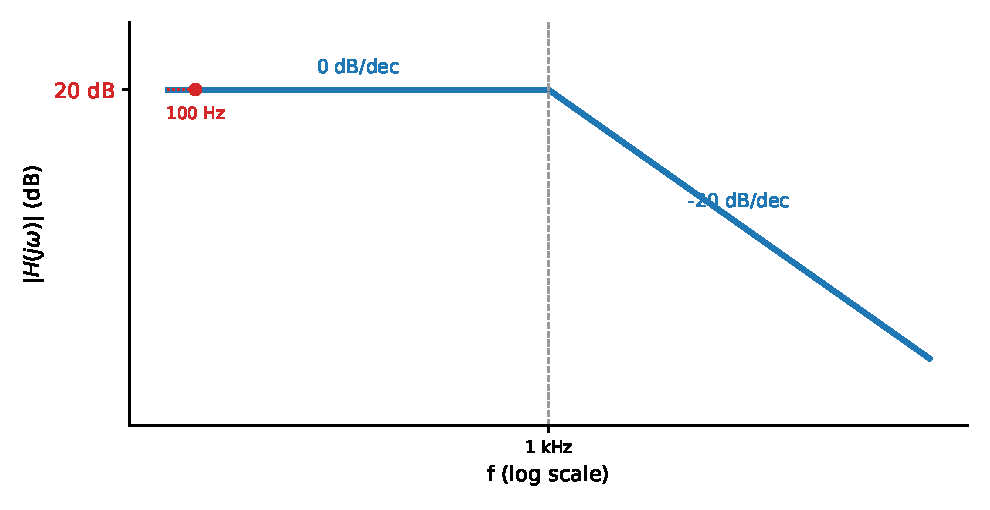
\includegraphics[width=0.8\linewidth,height=6cm,keepaspectratio]{p01_plot}\end{center}
\end{probbox}

\begin{probbox}{Problem 1D.2 \hfill Easy}
The straight-line (asymptotic) magnitude Bode plot of $H(s)=\dfrac{V_o(s)}{V_i(s)}$ is shown. (a) Find $H(s)$ (assume $K>0$ and no right-half-plane poles or zeros). (b) Find the steady-state output $V_o(t)$ for $V_i(t) = 1\sin\left(2\pi\cdot 100\,t\right)$.
\begin{center}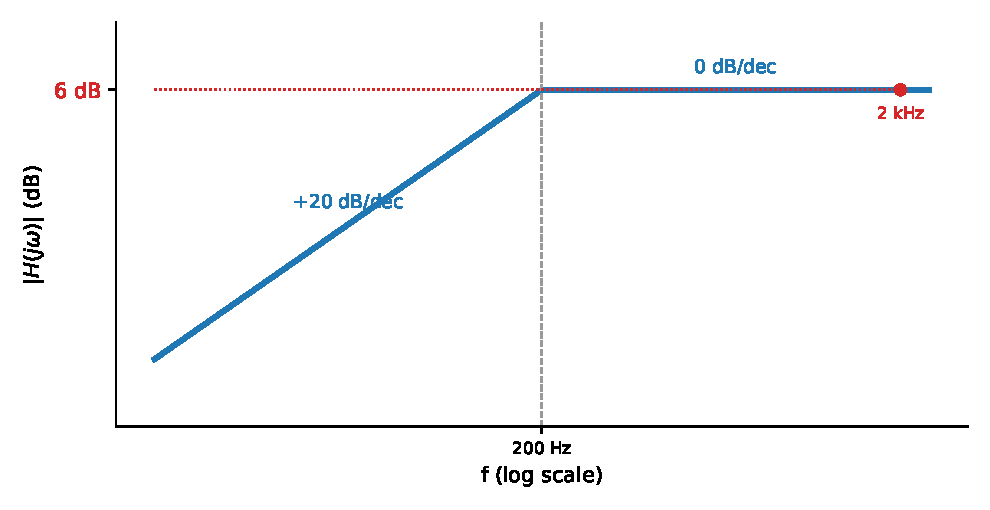
\includegraphics[width=0.8\linewidth,height=6cm,keepaspectratio]{p02_plot}\end{center}
\end{probbox}

\begin{probbox}{Problem 1D.3 \hfill Easy}
The straight-line (asymptotic) magnitude Bode plot of $H(s)=\dfrac{V_o(s)}{V_i(s)}$ is shown. (a) Find $H(s)$ (assume $K>0$ and no right-half-plane poles or zeros). (b) Find the steady-state output $V_o(t)$ for $V_i(t) = 2\cos\left(2\pi\cdot 10000\,t\right)$.
\begin{center}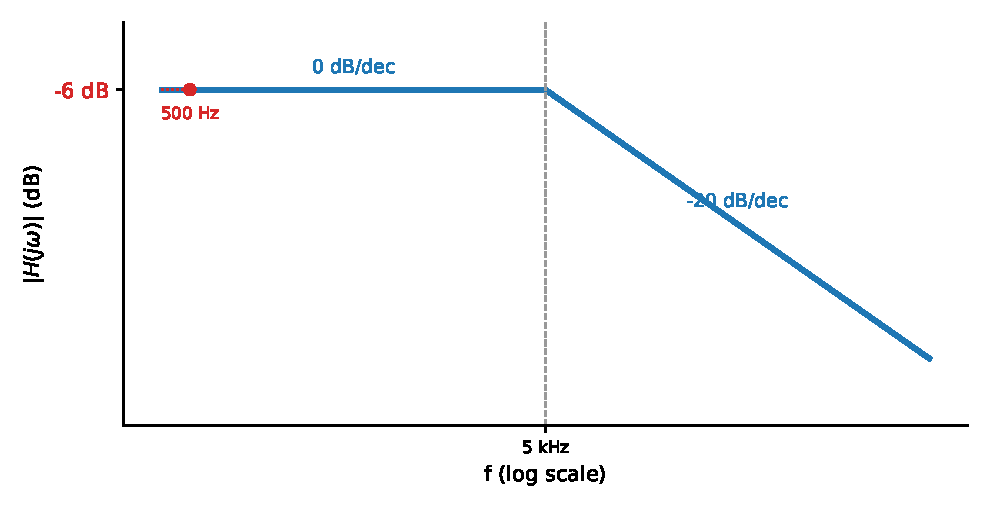
\includegraphics[width=0.8\linewidth,height=6cm,keepaspectratio]{p03_plot}\end{center}
\end{probbox}

\begin{probbox}{Problem 1D.4 \hfill Easy}
The straight-line (asymptotic) magnitude Bode plot of $H(s)=\dfrac{V_o(s)}{V_i(s)}$ is shown. (a) Find $H(s)$ (assume $K>0$ and no right-half-plane poles or zeros). (b) Find the steady-state output $V_o(t)$ for $V_i(t) = 1\sin\left(2\pi\cdot 1000\,t\right)$.
\begin{center}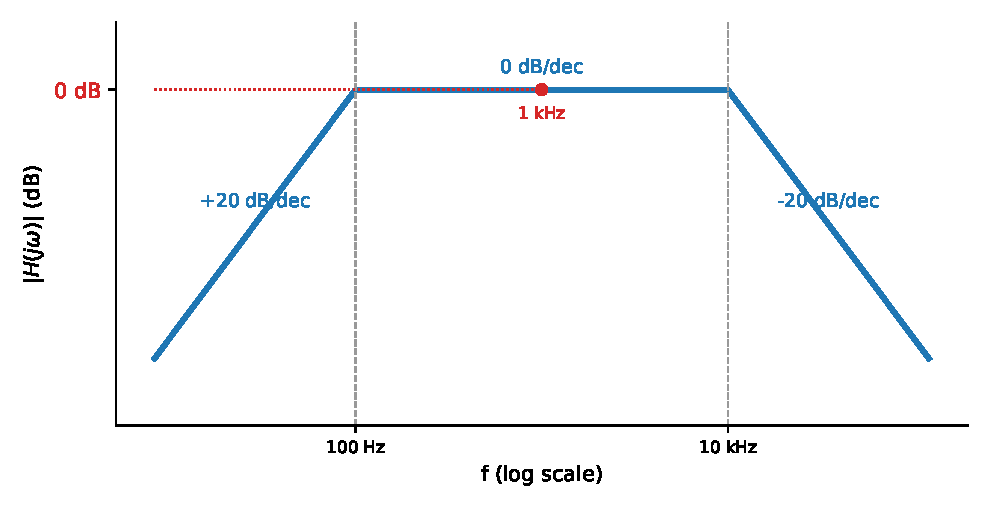
\includegraphics[width=0.8\linewidth,height=6cm,keepaspectratio]{p04_plot}\end{center}
\end{probbox}

\begin{probbox}{Problem 1D.5 \hfill Easy}
The straight-line (asymptotic) magnitude Bode plot of $H(s)=\dfrac{V_o(s)}{V_i(s)}$ is shown. (a) Find $H(s)$ (assume $K>0$ and no right-half-plane poles or zeros). (b) Find the steady-state output $V_o(t)$ for $V_i(t) = 0.5\sin\left(2\pi\cdot 3000\,t\right)$.
\begin{center}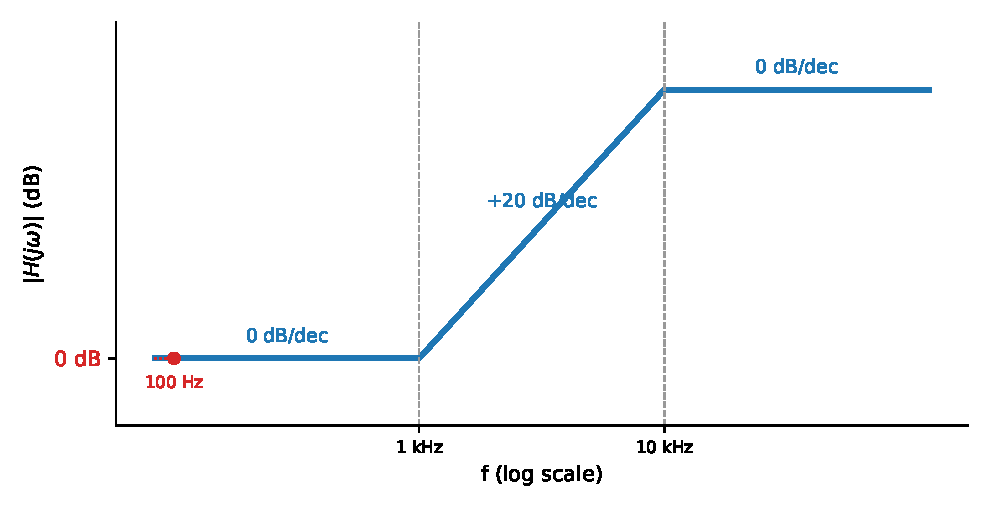
\includegraphics[width=0.8\linewidth,height=6cm,keepaspectratio]{p05_plot}\end{center}
\end{probbox}

\begin{probbox}{Problem 1D.6 \hfill Easy}
The straight-line (asymptotic) magnitude Bode plot of $H(s)=\dfrac{V_o(s)}{V_i(s)}$ is shown. (a) Find $H(s)$ (assume $K>0$ and no right-half-plane poles or zeros). (b) Find the steady-state output $V_o(t)$ for $V_i(t) = 1\sin\left(2\pi\cdot 500\,t\right)$.
\begin{center}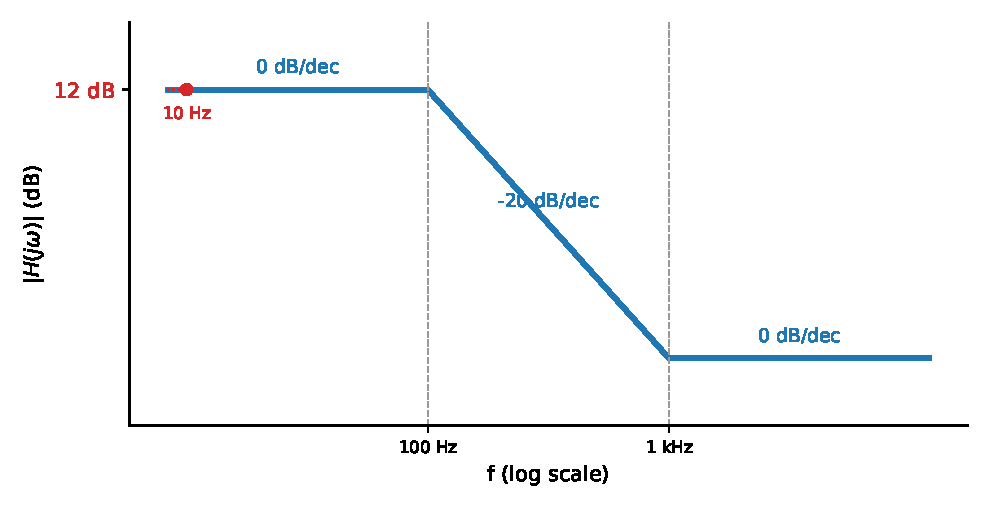
\includegraphics[width=0.8\linewidth,height=6cm,keepaspectratio]{p06_plot}\end{center}
\end{probbox}

\subsection*{Medium problems}
\begin{probbox}{Problem 1D.7 \hfill Medium}
The straight-line (asymptotic) magnitude Bode plot of $H(s)=\dfrac{V_o(s)}{V_i(s)}$ is shown. (a) Find $H(s)$ (assume $K>0$ and no right-half-plane poles or zeros). (b) Find the steady-state output $V_o(t)$ for $V_i(t) = 0.1\sin\left(2\pi\cdot 20000\,t\right)$.
\begin{center}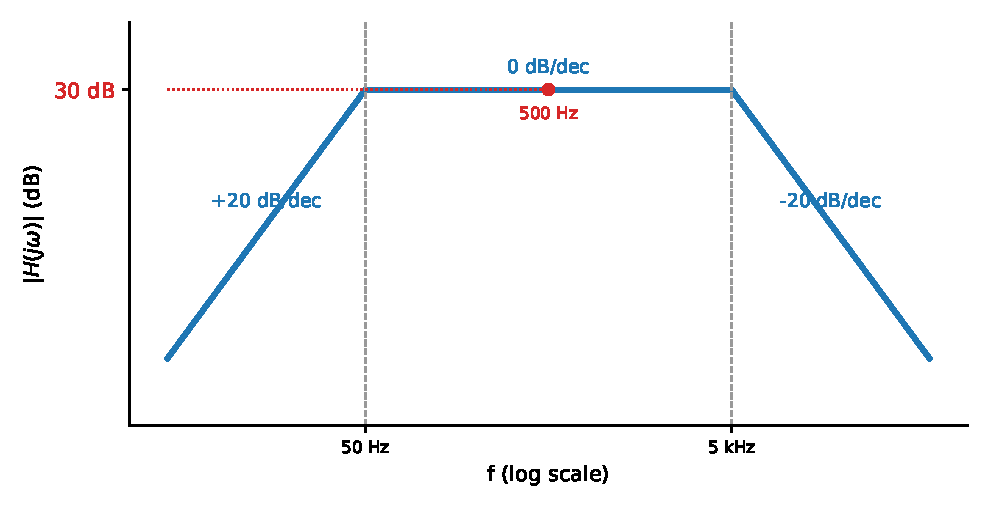
\includegraphics[width=0.8\linewidth,height=6cm,keepaspectratio]{p07_plot}\end{center}
\end{probbox}

\begin{probbox}{Problem 1D.8 \hfill Medium}
The straight-line (asymptotic) magnitude Bode plot of $H(s)=\dfrac{V_o(s)}{V_i(s)}$ is shown. (a) Find $H(s)$ (assume $K>0$ and no right-half-plane poles or zeros). (b) Find the steady-state output $V_o(t)$ for $V_i(t) = 0.05\sin\left(2\pi\cdot 5000\,t\right)$.
\begin{center}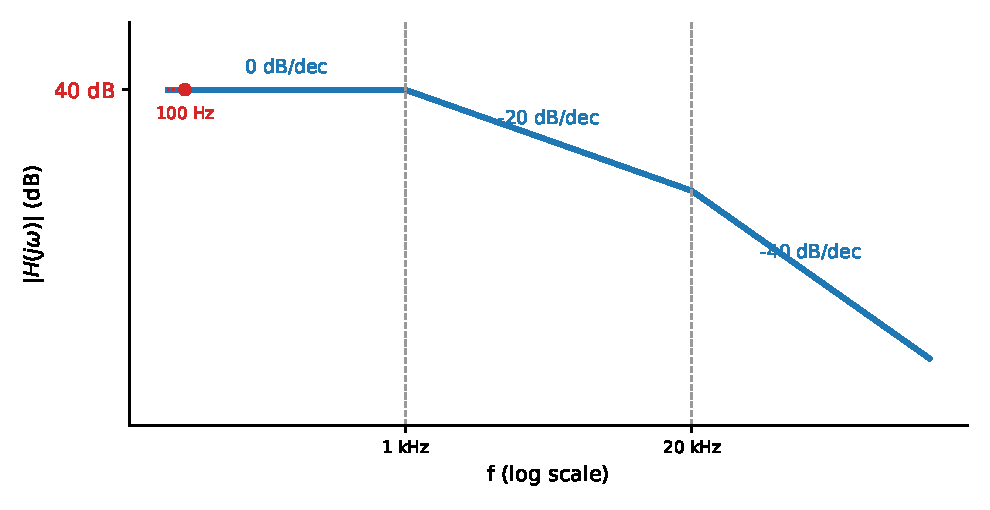
\includegraphics[width=0.8\linewidth,height=6cm,keepaspectratio]{p08_plot}\end{center}
\end{probbox}

\begin{probbox}{Problem 1D.9 \hfill Medium}
The straight-line (asymptotic) magnitude Bode plot of $H(s)=\dfrac{V_o(s)}{V_i(s)}$ is shown. (a) Find $H(s)$ (assume $K>0$ and no right-half-plane poles or zeros). (b) Find the steady-state output $V_o(t)$ for $V_i(t) = 0.2\sin\left(2\pi\cdot 1000\,t\right)$.
\begin{center}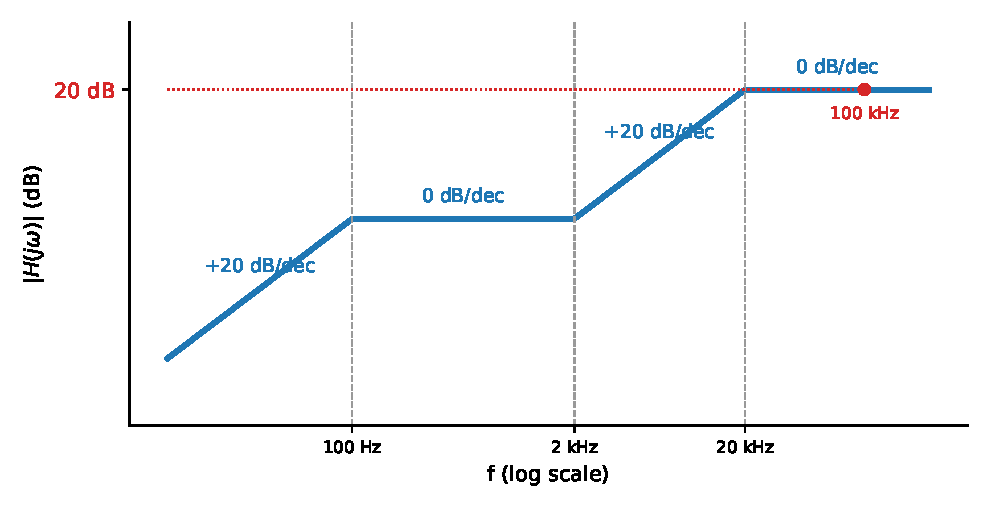
\includegraphics[width=0.8\linewidth,height=6cm,keepaspectratio]{p09_plot}\end{center}
\end{probbox}

\begin{probbox}{Problem 1D.10 \hfill Medium}
The straight-line (asymptotic) magnitude Bode plot of $H(s)=\dfrac{V_o(s)}{V_i(s)}$ is shown. (a) Find $H(s)$ (assume $K>0$ and no right-half-plane poles or zeros). (b) Find the steady-state output $V_o(t)$ for $V_i(t) = 0.5\sin\left(2\pi\cdot 400\,t\right)$.
\begin{center}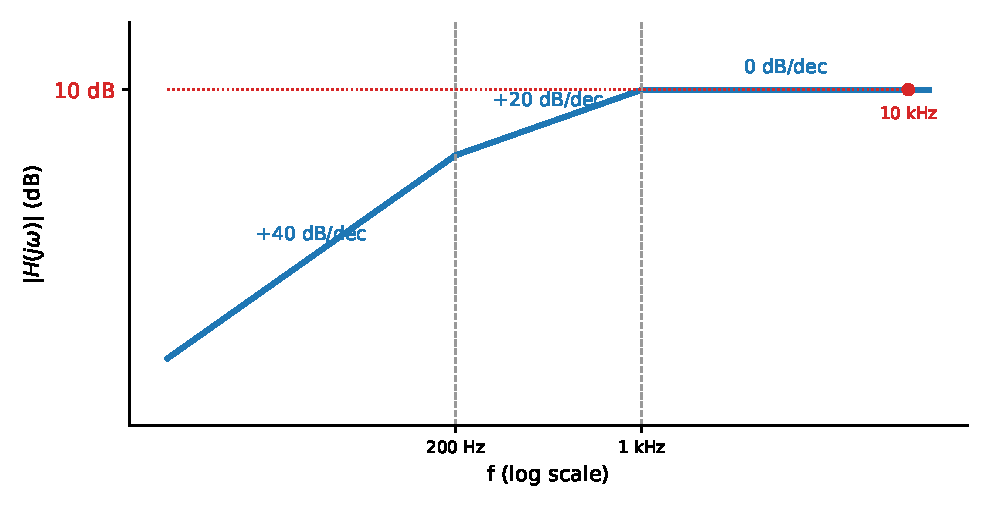
\includegraphics[width=0.8\linewidth,height=6cm,keepaspectratio]{p10_plot}\end{center}
\end{probbox}

\begin{probbox}{Problem 1D.11 \hfill Medium}
The straight-line (asymptotic) magnitude Bode plot of $H(s)=\dfrac{V_o(s)}{V_i(s)}$ is shown. (a) Find $H(s)$ (assume $K>0$ and no right-half-plane poles or zeros). (b) Find the steady-state output $V_o(t)$ for $V_i(t) = 1\sin\left(2\pi\cdot 4000\,t\right)$.
\begin{center}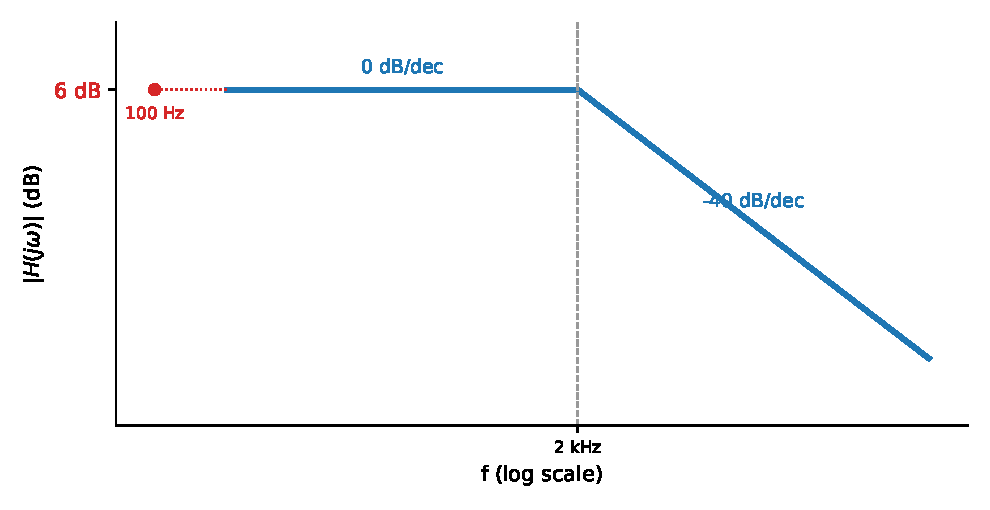
\includegraphics[width=0.8\linewidth,height=6cm,keepaspectratio]{p11_plot}\end{center}
\end{probbox}

\begin{probbox}{Problem 1D.12 \hfill Medium}
The straight-line (asymptotic) magnitude Bode plot of $H(s)=\dfrac{V_o(s)}{V_i(s)}$ is shown. (a) Find $H(s)$ (assume $K>0$ and no right-half-plane poles or zeros). (b) Find the steady-state output $V_o(t)$ for $V_i(t) = 1\sin\left(2\pi\cdot 2000\,t+\frac{\pi}{4}\right)$.
\begin{center}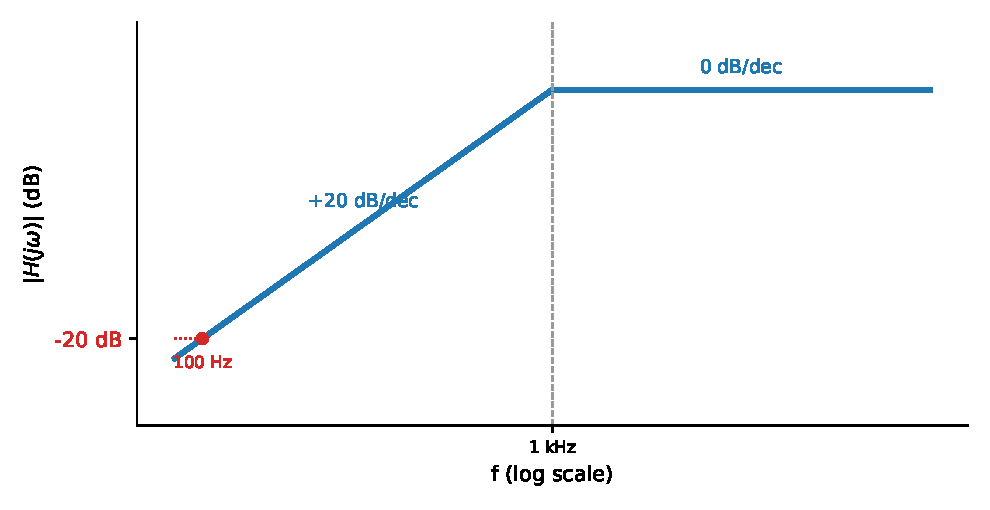
\includegraphics[width=0.8\linewidth,height=6cm,keepaspectratio]{p12_plot}\end{center}
\end{probbox}

\subsection*{Hard problems}
\begin{probbox}{Problem 1D.13 \hfill Hard}
The straight-line (asymptotic) magnitude Bode plot of $H(s)=\dfrac{V_o(s)}{V_i(s)}$ is shown. (a) Find $H(s)$ (assume $K>0$ and no right-half-plane poles or zeros). (b) Find the steady-state output $V_o(t)$ for $V_i(t) = 0.3\sin\left(2\pi\cdot 10000\,t\right)$.
\begin{center}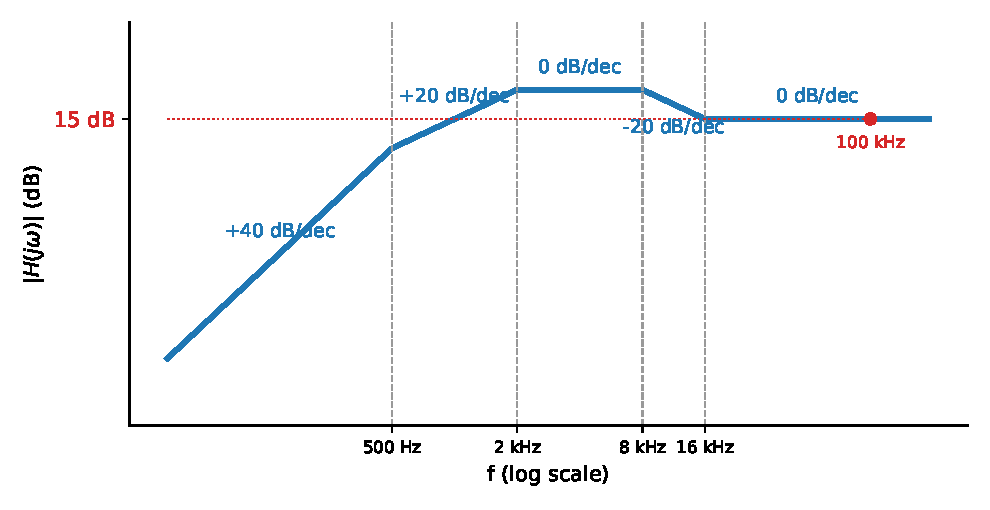
\includegraphics[width=0.8\linewidth,height=6cm,keepaspectratio]{p13_plot}\end{center}
\end{probbox}

\begin{probbox}{Problem 1D.14 \hfill Hard}
The straight-line (asymptotic) magnitude Bode plot of $H(s)=\dfrac{V_o(s)}{V_i(s)}$ is shown. (a) Find $H(s)$ (assume $K>0$ and no right-half-plane poles or zeros). (b) Find the steady-state output $V_o(t)$ for $V_i(t) = 0.2\sin\left(2\pi\cdot 2000\,t+\frac{\pi}{3}\right)$.
\begin{center}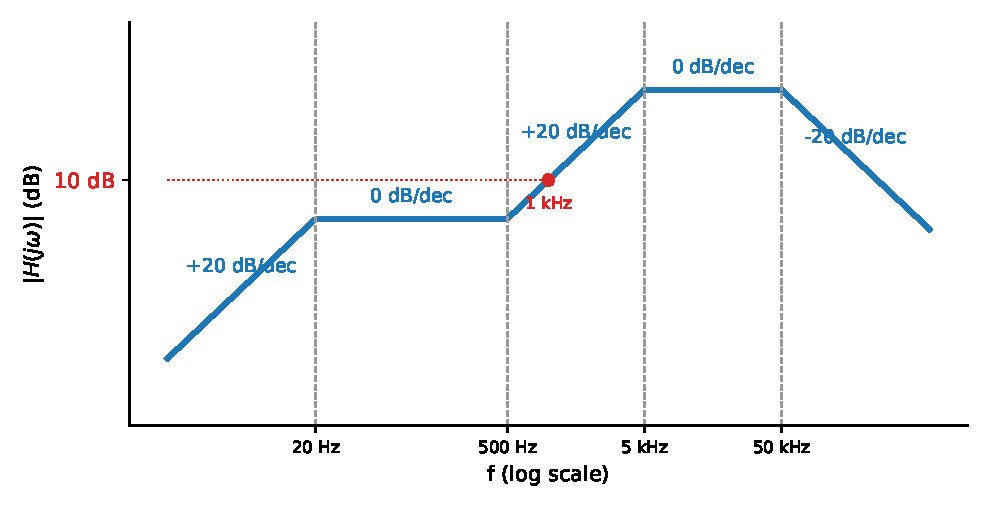
\includegraphics[width=0.8\linewidth,height=6cm,keepaspectratio]{p14_plot}\end{center}
\end{probbox}

\begin{probbox}{Problem 1D.15 \hfill Hard}
The straight-line (asymptotic) magnitude Bode plot of $H(s)=\dfrac{V_o(s)}{V_i(s)}$ is shown. (a) Find $H(s)$ (assume $K>0$ and no right-half-plane poles or zeros). (b) Find the steady-state output $V_o(t)$ for $V_i(t) = 0.1\sin\left(2\pi\cdot 300\,t\right)$.
\begin{center}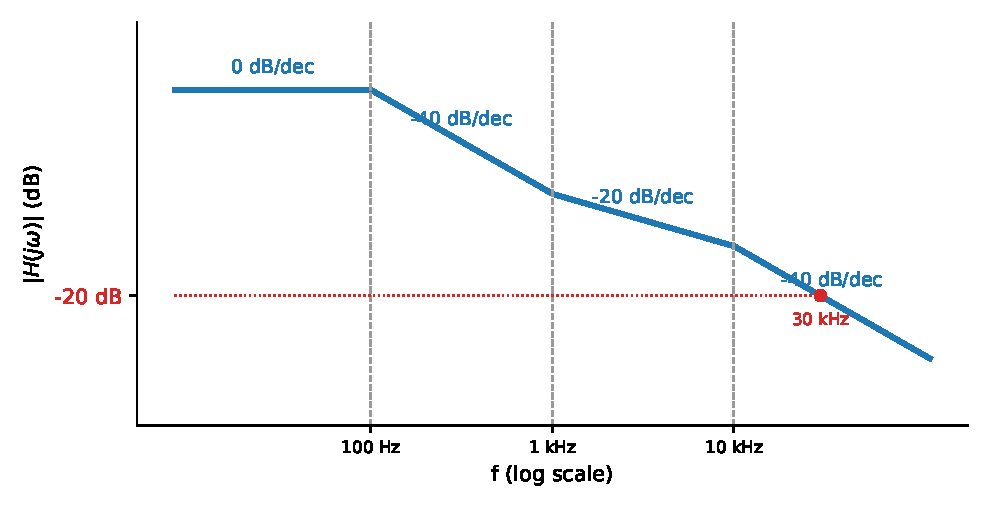
\includegraphics[width=0.8\linewidth,height=6cm,keepaspectratio]{p15_plot}\end{center}
\end{probbox}

\begin{probbox}{Problem 1D.16 \hfill Hard}
The straight-line (asymptotic) magnitude Bode plot of $H(s)=\dfrac{V_o(s)}{V_i(s)}$ is shown. (a) Find $H(s)$ (assume $K>0$ and no right-half-plane poles or zeros). (b) Find the steady-state output $V_o(t)$ for $V_i(t) = 0.05\cos\left(2\pi\cdot 1000\,t-\frac{\pi}{6}\right)$.
\begin{center}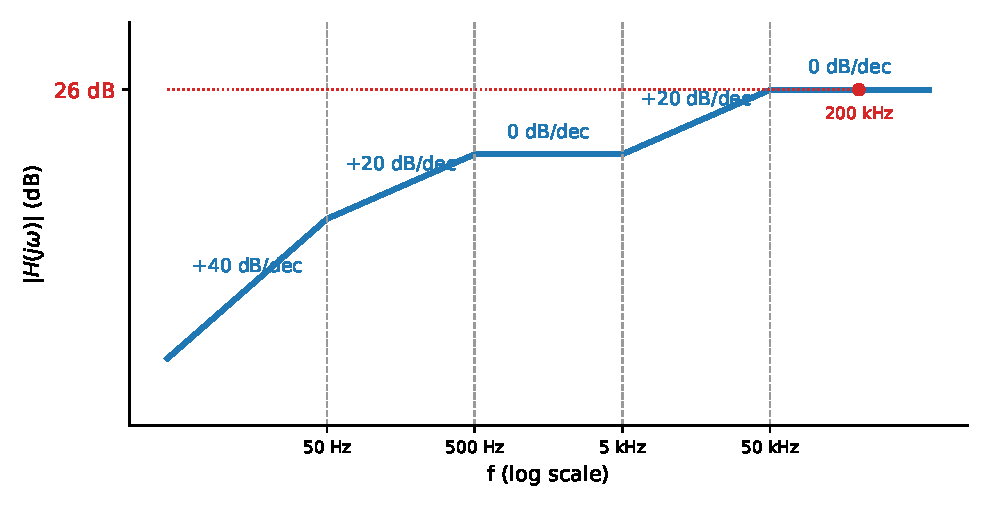
\includegraphics[width=0.8\linewidth,height=6cm,keepaspectratio]{p16_plot}\end{center}
\end{probbox}

\begin{probbox}{Problem 1D.17 \hfill Hard}
The straight-line (asymptotic) magnitude Bode plot of $H(s)=\dfrac{V_o(s)}{V_i(s)}$ is shown. (a) Find $H(s)$ (assume $K>0$ and no right-half-plane poles or zeros). (b) Find the steady-state output $V_o(t)$ for $V_i(t) = 0.02\sin\left(2\pi\cdot 5000\,t+\frac{\pi}{2}\right)$.
\begin{center}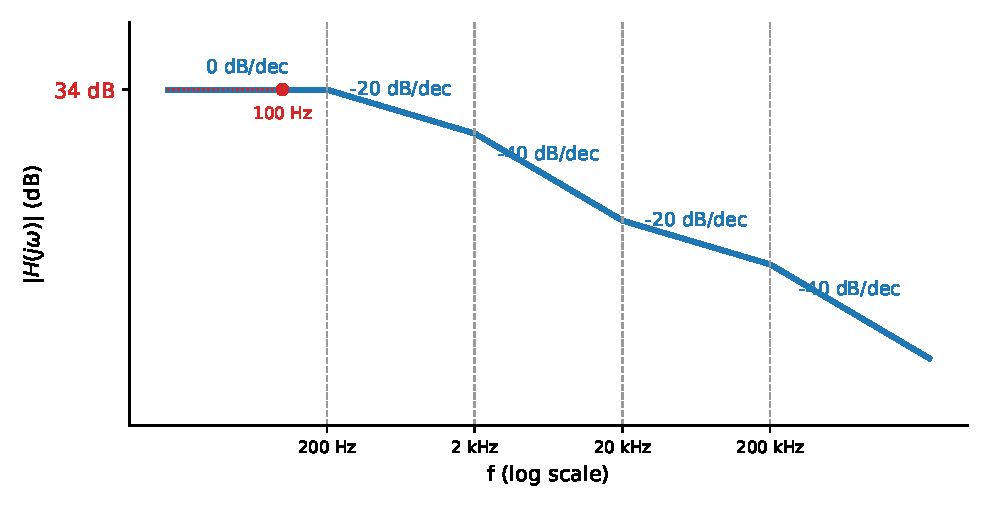
\includegraphics[width=0.8\linewidth,height=6cm,keepaspectratio]{p17_plot}\end{center}
\end{probbox}

\begin{probbox}{Problem 1D.18 \hfill Hard}
The straight-line (asymptotic) magnitude Bode plot of $H(s)=\dfrac{V_o(s)}{V_i(s)}$ is shown. (a) Find $H(s)$ (assume $K>0$ and no right-half-plane poles or zeros). (b) Find the steady-state output $V_o(t)$ for $V_i(t) = 0.5\sin\left(2\pi\cdot 3000\,t\right)$.
\begin{center}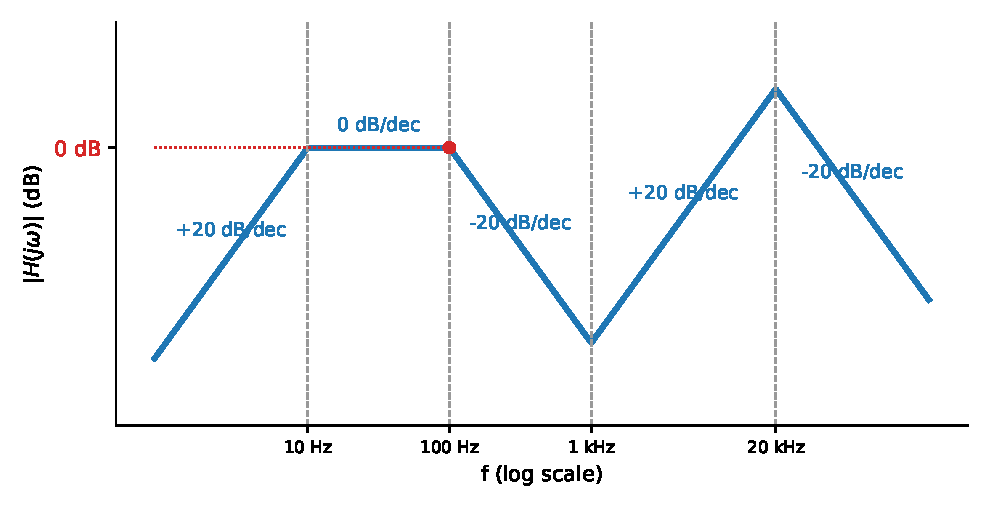
\includegraphics[width=0.8\linewidth,height=6cm,keepaspectratio]{p18_plot}\end{center}
\end{probbox}

\newpage
\section*{Solutions}
Every solution follows the same six steps of the pipeline card.
\newpage
\subsection*{Solution 1D.1 \hfill Easy}
\begin{center}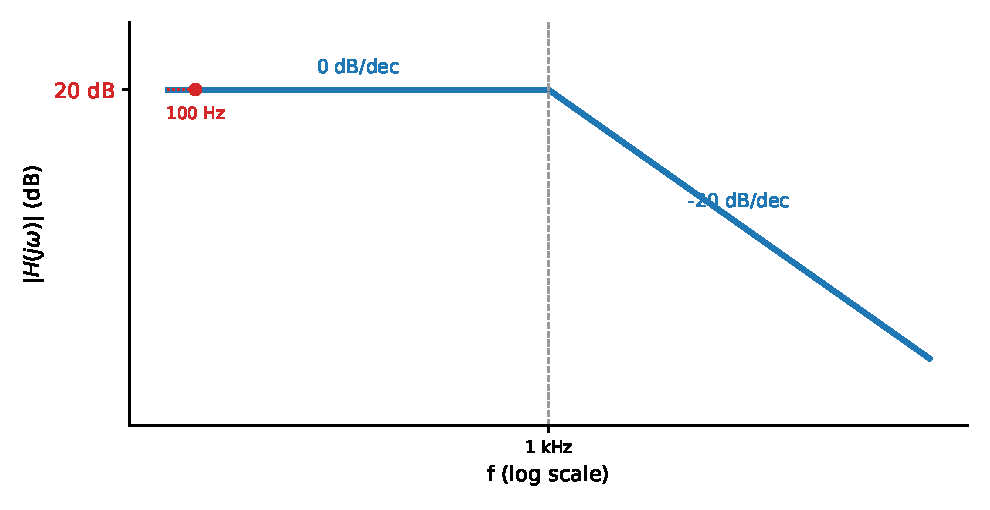
\includegraphics[width=0.7\linewidth,height=5cm,keepaspectratio]{p01_plot}\end{center}
\solstep{1}{Read the corners and slopes}Go left to right along the plot and write down the slope of every straight segment. At each corner frequency the slope changes by a multiple of 20\,dB/dec: every $-20$ is one pole, every $+20$ is one zero (tool T6 read backwards).\begin{center}\renewcommand{\arraystretch}{1.35}
\begin{tabular}{ccccl}
\toprule
corner $f_c$ & slope before & slope after & change & meaning \\
\midrule
1 kHz & $0$ & $-20$ & $-20$ & one pole at $f_c$ \\
\bottomrule
\end{tabular}\end{center}

\solstep{2}{Starting slope $\Rightarrow$ factors of $s$}The plot starts \emph{flat} (0\,dB/dec), so there is no factor $s$ in the numerator: every pole is written as $\frac{1}{1+s/p}$ and every zero as $\left(1+\frac{s}{z}\right)$, which are all $\approx1$ (0\,dB) at low frequency. Every corner is an angular frequency $\omega_c=2\pi f_c$.
\solstep{3}{Assemble $H(s)$}Put one factor per pole/zero in front of an unknown constant $K$:\[
H(s) = K\,\dfrac{1}{1+\dfrac{s}{2\pi\cdot 1\mathrm{k}}}
\]

\solstep{4}{Find $K$ from the marked level}The plot marks the level $20$\,dB at $f=$\,100 Hz. On the straight-line plot every factor is either exactly 0\,dB (where it is $\approx1$) or a $\pm20$\,dB/dec line, so evaluate the \emph{asymptote} of each factor at that frequency (the level of a line with slope $\pm20$\,dB/dec is $\pm20\log_{10}(f/f_c)$):\begin{center}\renewcommand{\arraystretch}{1.35}
\begin{tabular}{cccc}
\toprule
factor & $f_c$ & at $f=$\,100 Hz & asymptote (dB) \\
\midrule
$\rule[-1.7em]{0pt}{4em}\dfrac{1}{1+\dfrac{s}{2\pi\cdot 1\mathrm{k}}}$ & 1 kHz & $f<f_c$: $\approx 1$ & $0$ \\
\textbf{sum} &  &  & $\mathbf{0}$ \\
\bottomrule
\end{tabular}\end{center}
The dB values of the factors \emph{add} (magnitudes multiply), so\[
20\log_{10}K = 20 - (0) = 20\ \mathrm{dB}\quad\Rightarrow\quad K = 10^{20/20} = 10
\]

So\[
\boxed{H(s) = 10\,\dfrac{1}{1+\dfrac{s}{2\pi\cdot 1\mathrm{k}}}}
\]

\solstep{5}{Check}Rebuild the plot from the factors: each factor's straight-line plot (green) is added to get $|H|$ (blue). It must reproduce every slope of the given plot and the marked level.\begin{center}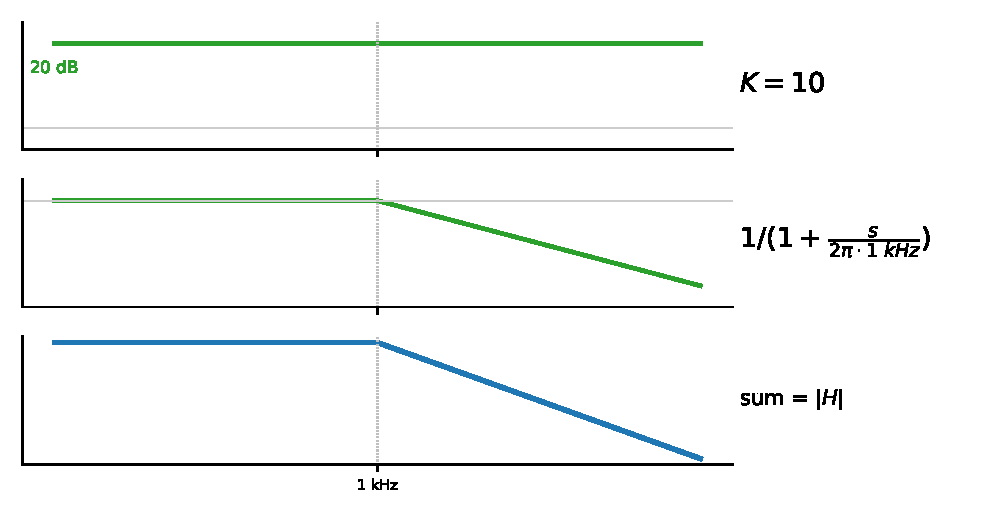
\includegraphics[width=0.82\linewidth,height=9cm,keepaspectratio]{p01_factors}\end{center}
\begin{center}\renewcommand{\arraystretch}{1.35}
\begin{tabular}{lcl}
\toprule
frequency range & slope & asymptote level \\
\midrule
$f<$ 1 kHz & $0$ dB/dec & 20 dB at end \\
$f>$ 1 kHz & $-20$ dB/dec & 20 dB at start \\
\bottomrule
\end{tabular}\end{center}

\solstep{6}{Steady-state output}The input is $V_i(t) = 0.5\sin\left(2\pi\cdot 2000\,t\right)$, so $\omega_{in} = 2\pi\cdot 2000 = 12600$\,rad/s. Put $s=j\omega_{in}$ in each factor (tool T5; use the \emph{exact} factors here, not the straight lines): magnitudes multiply, angles add.
{\small Rules: $\left|\frac{s}{s+p}\right| = \frac{\omega}{\sqrt{\omega^2+p^2}}$, $\angle = \frac{\pi}{2}-\tan^{-1}\frac{\omega}{p}$;\quad $\left|\frac{1}{1+s/p}\right| = \frac{1}{\sqrt{1+(\omega/p)^2}}$, $\angle = -\tan^{-1}\frac{\omega}{p}$;\quad $\left|1+\frac{s}{z}\right| = \sqrt{1+(\omega/z)^2}$, $\angle = \tan^{-1}\frac{\omega}{z}$;\quad a negative $K$ adds $-\pi$.}
\begin{center}\renewcommand{\arraystretch}{1.35}
\begin{tabular}{ccc}
\toprule
factor & magnitude & angle (rad) \\
\midrule
$10$ & $10$ & $0$ \\
$\rule[-1.7em]{0pt}{4em}\dfrac{1}{1+\dfrac{s}{2\pi\cdot 1\mathrm{k}}}$ & $0.4472$ & $-1.11$ \\
\textbf{total} & $\mathbf{4.472}$ (product) & $\mathbf{-1.11}$ (sum) \\
\bottomrule
\end{tabular}\end{center}

\begin{align*}
|H(j\omega_{in})| &= 4.47, \qquad \angle H(j\omega_{in}) = -1.11\ \mathrm{rad} \\
v_{o,ac}(t) &= 4.47\times 0.5\,\sin\left(2\pi\cdot 2000\,t - 1.11\right) = 2.24\,\sin\left(2\pi\cdot 2000\,t - 1.11\right)
\end{align*}

\[
\boxed{V_o(t) = 2.24\,\sin\left(2\pi\cdot 2000\,t - 1.11\right)\ \mathrm{V}}
\]

\begin{ansbox}
$H(s) = 10\,\dfrac{1}{1+\dfrac{s}{2\pi\cdot 1\mathrm{k}}}$\quad (corners: 1 kHz)\\[4pt]
$V_o(t) = 2.24\,\sin\left(2\pi\cdot 2000\,t - 1.11\right)\ \mathrm{V}$
\end{ansbox}

\newpage
\subsection*{Solution 1D.2 \hfill Easy}
\begin{center}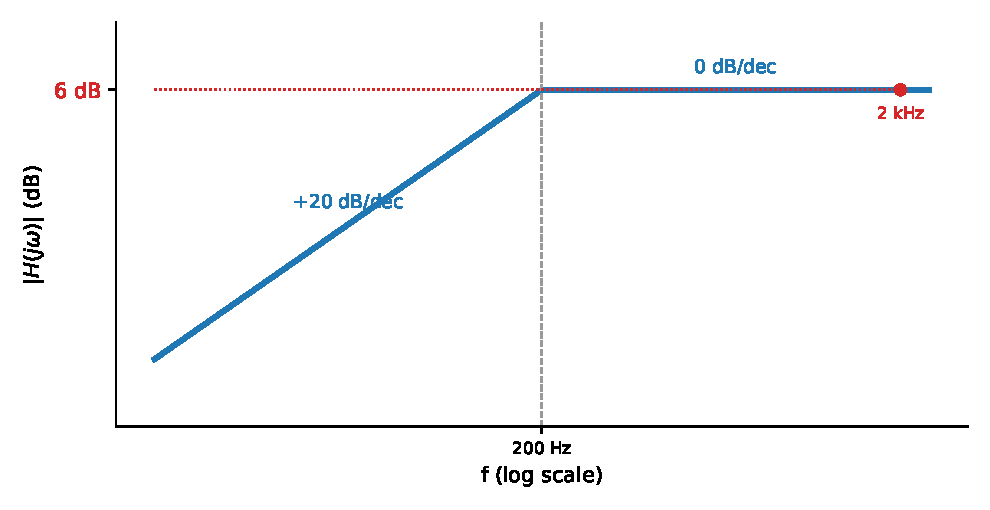
\includegraphics[width=0.7\linewidth,height=5cm,keepaspectratio]{p02_plot}\end{center}
\solstep{1}{Read the corners and slopes}Go left to right along the plot and write down the slope of every straight segment. At each corner frequency the slope changes by a multiple of 20\,dB/dec: every $-20$ is one pole, every $+20$ is one zero (tool T6 read backwards).\begin{center}\renewcommand{\arraystretch}{1.35}
\begin{tabular}{ccccl}
\toprule
corner $f_c$ & slope before & slope after & change & meaning \\
\midrule
200 Hz & $+20$ & $0$ & $-20$ & one pole at $f_c$ \\
\bottomrule
\end{tabular}\end{center}

\solstep{2}{Starting slope $\Rightarrow$ factors of $s$}The plot starts with a slope of $+20$\,dB/dec, i.e. $|H|\propto\omega^1$ at low frequency: the numerator contains $s$. As in class, pair each $s$ with one of the \emph{lowest} poles (200 Hz) as $\frac{s}{s+p}$: such a factor rises at $+20$\,dB/dec below $p$ and is $\approx1$ (0\,dB) above it. The remaining poles are written $\frac{1}{1+s/p}$ and the zeros $\left(1+\frac{s}{z}\right)$. Every corner is an angular frequency $\omega_c=2\pi f_c$.
\solstep{3}{Assemble $H(s)$}Put one factor per pole/zero in front of an unknown constant $K$:\[
H(s) = K\,\dfrac{s}{s+2\pi\cdot 200}
\]

\solstep{4}{Find $K$ from the marked level}The plot marks the level $6$\,dB at $f=$\,2 kHz. On the straight-line plot every factor is either exactly 0\,dB (where it is $\approx1$) or a $\pm20$\,dB/dec line, so evaluate the \emph{asymptote} of each factor at that frequency (the level of a line with slope $\pm20$\,dB/dec is $\pm20\log_{10}(f/f_c)$):\begin{center}\renewcommand{\arraystretch}{1.35}
\begin{tabular}{cccc}
\toprule
factor & $f_c$ & at $f=$\,2 kHz & asymptote (dB) \\
\midrule
$\rule[-1.1em]{0pt}{2.8em}\dfrac{s}{s+2\pi\cdot 200}$ & 200 Hz & $f>f_c$: $\approx 1$ & $0$ \\
\textbf{sum} &  &  & $\mathbf{0}$ \\
\bottomrule
\end{tabular}\end{center}
The dB values of the factors \emph{add} (magnitudes multiply), so\[
20\log_{10}K = 6 - (0) = 6\ \mathrm{dB}\quad\Rightarrow\quad K = 10^{6/20} = 2
\]

So\[
\boxed{H(s) = 2\,\dfrac{s}{s+2\pi\cdot 200}}
\]

\solstep{5}{Check}Rebuild the plot from the factors: each factor's straight-line plot (green) is added to get $|H|$ (blue). It must reproduce every slope of the given plot and the marked level.\begin{center}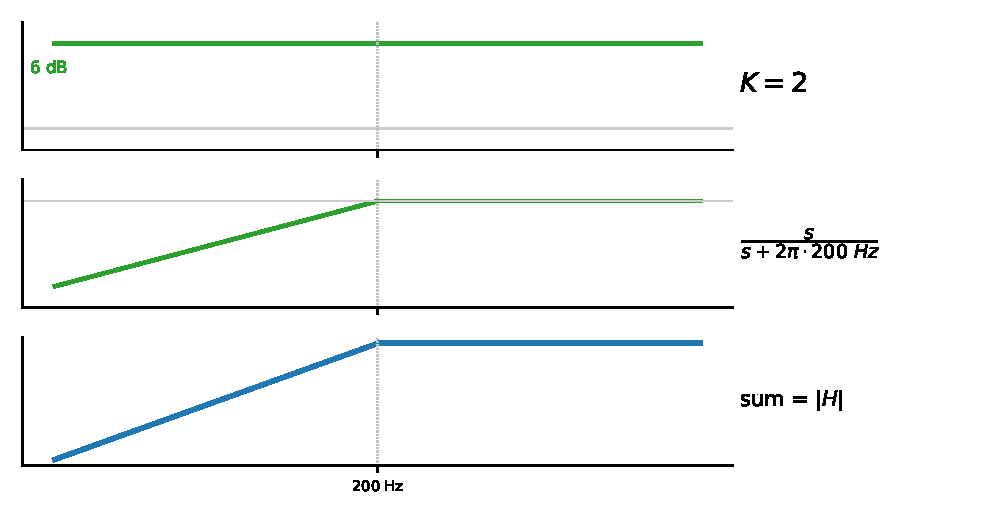
\includegraphics[width=0.82\linewidth,height=9cm,keepaspectratio]{p02_factors}\end{center}
\begin{center}\renewcommand{\arraystretch}{1.35}
\begin{tabular}{lcl}
\toprule
frequency range & slope & asymptote level \\
\midrule
$f<$ 200 Hz & $+20$ dB/dec & 6 dB at end \\
$f>$ 200 Hz & $0$ dB/dec & 6 dB at start \\
\bottomrule
\end{tabular}\end{center}

\solstep{6}{Steady-state output}The input is $V_i(t) = 1\sin\left(2\pi\cdot 100\,t\right)$, so $\omega_{in} = 2\pi\cdot 100 = 628$\,rad/s. Put $s=j\omega_{in}$ in each factor (tool T5; use the \emph{exact} factors here, not the straight lines): magnitudes multiply, angles add.
{\small Rules: $\left|\frac{s}{s+p}\right| = \frac{\omega}{\sqrt{\omega^2+p^2}}$, $\angle = \frac{\pi}{2}-\tan^{-1}\frac{\omega}{p}$;\quad $\left|\frac{1}{1+s/p}\right| = \frac{1}{\sqrt{1+(\omega/p)^2}}$, $\angle = -\tan^{-1}\frac{\omega}{p}$;\quad $\left|1+\frac{s}{z}\right| = \sqrt{1+(\omega/z)^2}$, $\angle = \tan^{-1}\frac{\omega}{z}$;\quad a negative $K$ adds $-\pi$.}
\begin{center}\renewcommand{\arraystretch}{1.35}
\begin{tabular}{ccc}
\toprule
factor & magnitude & angle (rad) \\
\midrule
$2$ & $1.995$ & $0$ \\
$\rule[-1.1em]{0pt}{2.8em}\dfrac{s}{s+2\pi\cdot 200}$ & $0.4472$ & $1.11$ \\
\textbf{total} & $\mathbf{0.8923}$ (product) & $\mathbf{1.11}$ (sum) \\
\bottomrule
\end{tabular}\end{center}

\begin{align*}
|H(j\omega_{in})| &= 0.892, \qquad \angle H(j\omega_{in}) = 1.11\ \mathrm{rad} \\
v_{o,ac}(t) &= 0.892\times 1\,\sin\left(2\pi\cdot 100\,t + 1.11\right) = 0.892\,\sin\left(2\pi\cdot 100\,t + 1.11\right)
\end{align*}

\[
\boxed{V_o(t) = 0.892\,\sin\left(2\pi\cdot 100\,t + 1.11\right)\ \mathrm{V}}
\]

\begin{ansbox}
$H(s) = 2\,\dfrac{s}{s+2\pi\cdot 200}$\quad (corners: 200 Hz)\\[4pt]
$V_o(t) = 0.892\,\sin\left(2\pi\cdot 100\,t + 1.11\right)\ \mathrm{V}$
\end{ansbox}

\newpage
\subsection*{Solution 1D.3 \hfill Easy}
\begin{center}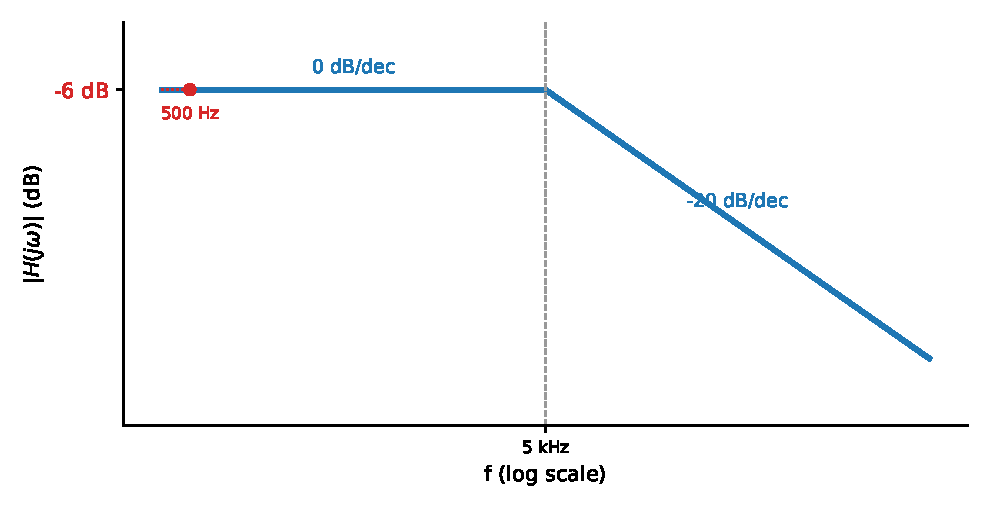
\includegraphics[width=0.7\linewidth,height=5cm,keepaspectratio]{p03_plot}\end{center}
\solstep{1}{Read the corners and slopes}Go left to right along the plot and write down the slope of every straight segment. At each corner frequency the slope changes by a multiple of 20\,dB/dec: every $-20$ is one pole, every $+20$ is one zero (tool T6 read backwards).\begin{center}\renewcommand{\arraystretch}{1.35}
\begin{tabular}{ccccl}
\toprule
corner $f_c$ & slope before & slope after & change & meaning \\
\midrule
5 kHz & $0$ & $-20$ & $-20$ & one pole at $f_c$ \\
\bottomrule
\end{tabular}\end{center}

\solstep{2}{Starting slope $\Rightarrow$ factors of $s$}The plot starts \emph{flat} (0\,dB/dec), so there is no factor $s$ in the numerator: every pole is written as $\frac{1}{1+s/p}$ and every zero as $\left(1+\frac{s}{z}\right)$, which are all $\approx1$ (0\,dB) at low frequency. Every corner is an angular frequency $\omega_c=2\pi f_c$.
\solstep{3}{Assemble $H(s)$}Put one factor per pole/zero in front of an unknown constant $K$:\[
H(s) = K\,\dfrac{1}{1+\dfrac{s}{2\pi\cdot 5\mathrm{k}}}
\]

\solstep{4}{Find $K$ from the marked level}The plot marks the level $-6$\,dB at $f=$\,500 Hz. On the straight-line plot every factor is either exactly 0\,dB (where it is $\approx1$) or a $\pm20$\,dB/dec line, so evaluate the \emph{asymptote} of each factor at that frequency (the level of a line with slope $\pm20$\,dB/dec is $\pm20\log_{10}(f/f_c)$):\begin{center}\renewcommand{\arraystretch}{1.35}
\begin{tabular}{cccc}
\toprule
factor & $f_c$ & at $f=$\,500 Hz & asymptote (dB) \\
\midrule
$\rule[-1.7em]{0pt}{4em}\dfrac{1}{1+\dfrac{s}{2\pi\cdot 5\mathrm{k}}}$ & 5 kHz & $f<f_c$: $\approx 1$ & $0$ \\
\textbf{sum} &  &  & $\mathbf{0}$ \\
\bottomrule
\end{tabular}\end{center}
The dB values of the factors \emph{add} (magnitudes multiply), so\[
20\log_{10}K = -6 - (0) = -6\ \mathrm{dB}\quad\Rightarrow\quad K = 10^{-6/20} = 0.501
\]

So\[
\boxed{H(s) = 0.501\,\dfrac{1}{1+\dfrac{s}{2\pi\cdot 5\mathrm{k}}}}
\]

\solstep{5}{Check}Rebuild the plot from the factors: each factor's straight-line plot (green) is added to get $|H|$ (blue). It must reproduce every slope of the given plot and the marked level.\begin{center}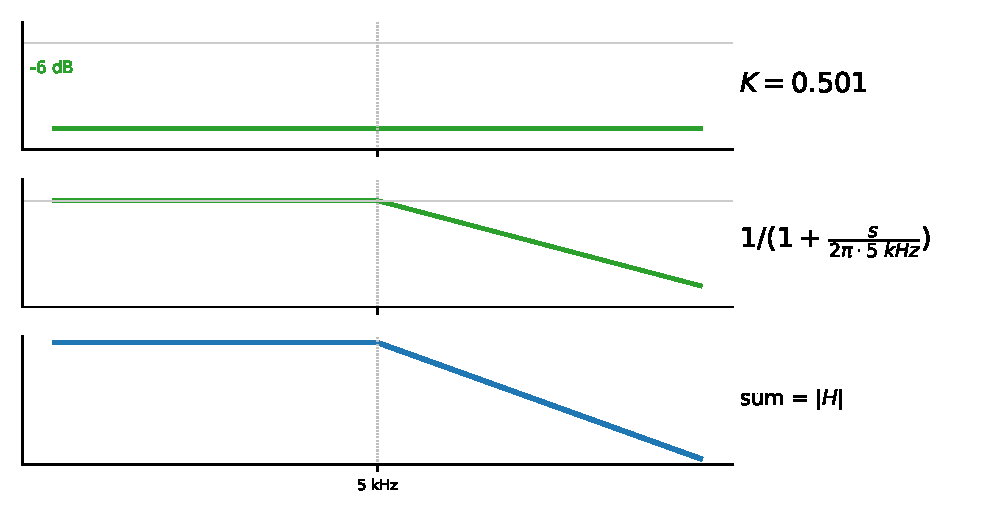
\includegraphics[width=0.82\linewidth,height=9cm,keepaspectratio]{p03_factors}\end{center}
\begin{center}\renewcommand{\arraystretch}{1.35}
\begin{tabular}{lcl}
\toprule
frequency range & slope & asymptote level \\
\midrule
$f<$ 5 kHz & $0$ dB/dec & -6 dB at end \\
$f>$ 5 kHz & $-20$ dB/dec & -6 dB at start \\
\bottomrule
\end{tabular}\end{center}

\solstep{6}{Steady-state output}The input is $V_i(t) = 2\cos\left(2\pi\cdot 10000\,t\right)$, so $\omega_{in} = 2\pi\cdot 10000 = 62800$\,rad/s. Put $s=j\omega_{in}$ in each factor (tool T5; use the \emph{exact} factors here, not the straight lines): magnitudes multiply, angles add.
{\small Rules: $\left|\frac{s}{s+p}\right| = \frac{\omega}{\sqrt{\omega^2+p^2}}$, $\angle = \frac{\pi}{2}-\tan^{-1}\frac{\omega}{p}$;\quad $\left|\frac{1}{1+s/p}\right| = \frac{1}{\sqrt{1+(\omega/p)^2}}$, $\angle = -\tan^{-1}\frac{\omega}{p}$;\quad $\left|1+\frac{s}{z}\right| = \sqrt{1+(\omega/z)^2}$, $\angle = \tan^{-1}\frac{\omega}{z}$;\quad a negative $K$ adds $-\pi$.}
\begin{center}\renewcommand{\arraystretch}{1.35}
\begin{tabular}{ccc}
\toprule
factor & magnitude & angle (rad) \\
\midrule
$0.501$ & $0.5012$ & $0$ \\
$\rule[-1.7em]{0pt}{4em}\dfrac{1}{1+\dfrac{s}{2\pi\cdot 5\mathrm{k}}}$ & $0.4472$ & $-1.11$ \\
\textbf{total} & $\mathbf{0.2241}$ (product) & $\mathbf{-1.11}$ (sum) \\
\bottomrule
\end{tabular}\end{center}

\begin{align*}
|H(j\omega_{in})| &= 0.224, \qquad \angle H(j\omega_{in}) = -1.11\ \mathrm{rad} \\
v_{o,ac}(t) &= 0.224\times 2\,\cos\left(2\pi\cdot 10000\,t - 1.11\right) = 0.448\,\cos\left(2\pi\cdot 10000\,t - 1.11\right)
\end{align*}

\[
\boxed{V_o(t) = 0.448\,\cos\left(2\pi\cdot 10000\,t - 1.11\right)\ \mathrm{V}}
\]

\begin{ansbox}
$H(s) = 0.501\,\dfrac{1}{1+\dfrac{s}{2\pi\cdot 5\mathrm{k}}}$\quad (corners: 5 kHz)\\[4pt]
$V_o(t) = 0.448\,\cos\left(2\pi\cdot 10000\,t - 1.11\right)\ \mathrm{V}$
\end{ansbox}

\newpage
\subsection*{Solution 1D.4 \hfill Easy}
\begin{center}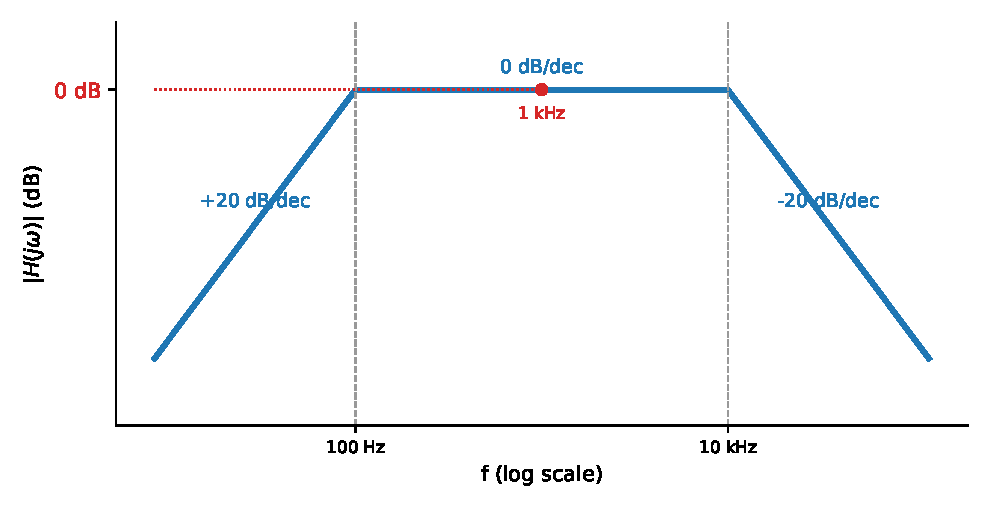
\includegraphics[width=0.7\linewidth,height=5cm,keepaspectratio]{p04_plot}\end{center}
\solstep{1}{Read the corners and slopes}Go left to right along the plot and write down the slope of every straight segment. At each corner frequency the slope changes by a multiple of 20\,dB/dec: every $-20$ is one pole, every $+20$ is one zero (tool T6 read backwards).\begin{center}\renewcommand{\arraystretch}{1.35}
\begin{tabular}{ccccl}
\toprule
corner $f_c$ & slope before & slope after & change & meaning \\
\midrule
100 Hz & $+20$ & $0$ & $-20$ & one pole at $f_c$ \\
10 kHz & $0$ & $-20$ & $-20$ & one pole at $f_c$ \\
\bottomrule
\end{tabular}\end{center}

\solstep{2}{Starting slope $\Rightarrow$ factors of $s$}The plot starts with a slope of $+20$\,dB/dec, i.e. $|H|\propto\omega^1$ at low frequency: the numerator contains $s$. As in class, pair each $s$ with one of the \emph{lowest} poles (100 Hz) as $\frac{s}{s+p}$: such a factor rises at $+20$\,dB/dec below $p$ and is $\approx1$ (0\,dB) above it. The remaining poles are written $\frac{1}{1+s/p}$ and the zeros $\left(1+\frac{s}{z}\right)$. Every corner is an angular frequency $\omega_c=2\pi f_c$.
\solstep{3}{Assemble $H(s)$}Put one factor per pole/zero in front of an unknown constant $K$:\[
H(s) = K\,\dfrac{s}{s+2\pi\cdot 100}\,\dfrac{1}{1+\dfrac{s}{2\pi\cdot 10\mathrm{k}}}
\]

\solstep{4}{Find $K$ from the marked level}The plot marks the level $0$\,dB at $f=$\,1 kHz. On the straight-line plot every factor is either exactly 0\,dB (where it is $\approx1$) or a $\pm20$\,dB/dec line, so evaluate the \emph{asymptote} of each factor at that frequency (the level of a line with slope $\pm20$\,dB/dec is $\pm20\log_{10}(f/f_c)$):\begin{center}\renewcommand{\arraystretch}{1.35}
\begin{tabular}{cccc}
\toprule
factor & $f_c$ & at $f=$\,1 kHz & asymptote (dB) \\
\midrule
$\rule[-1.1em]{0pt}{2.8em}\dfrac{s}{s+2\pi\cdot 100}$ & 100 Hz & $f>f_c$: $\approx 1$ & $0$ \\
$\rule[-1.7em]{0pt}{4em}\dfrac{1}{1+\dfrac{s}{2\pi\cdot 10\mathrm{k}}}$ & 10 kHz & $f<f_c$: $\approx 1$ & $0$ \\
\textbf{sum} &  &  & $\mathbf{0}$ \\
\bottomrule
\end{tabular}\end{center}
The dB values of the factors \emph{add} (magnitudes multiply), so\[
20\log_{10}K = 0 - (0) = 0\ \mathrm{dB}\quad\Rightarrow\quad K = 10^{0/20} = 1
\]

So\[
\boxed{H(s) = 1\,\dfrac{s}{s+2\pi\cdot 100}\,\dfrac{1}{1+\dfrac{s}{2\pi\cdot 10\mathrm{k}}}}
\]

\solstep{5}{Check}Rebuild the plot from the factors: each factor's straight-line plot (green) is added to get $|H|$ (blue). It must reproduce every slope of the given plot and the marked level.\begin{center}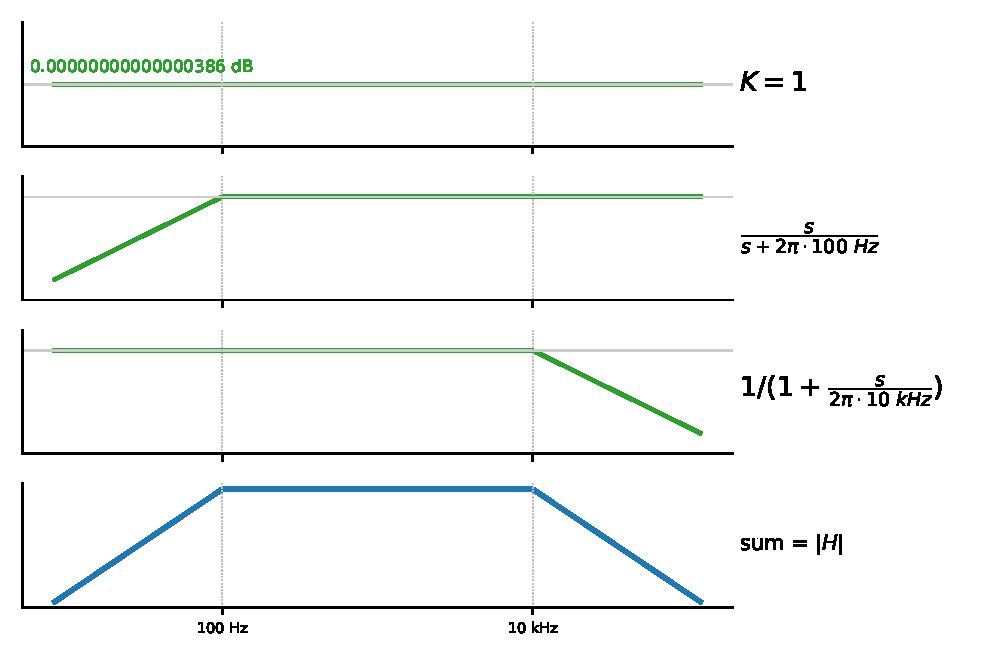
\includegraphics[width=0.82\linewidth,height=9cm,keepaspectratio]{p04_factors}\end{center}
\begin{center}\renewcommand{\arraystretch}{1.35}
\begin{tabular}{lcl}
\toprule
frequency range & slope & asymptote level \\
\midrule
$f<$ 100 Hz & $+20$ dB/dec & 0 dB at end \\
100 Hz -- 10 kHz & $0$ dB/dec & 0 dB at start, 0 dB at end \\
$f>$ 10 kHz & $-20$ dB/dec & 0 dB at start \\
\bottomrule
\end{tabular}\end{center}

\solstep{6}{Steady-state output}The input is $V_i(t) = 1\sin\left(2\pi\cdot 1000\,t\right)$, so $\omega_{in} = 2\pi\cdot 1000 = 6280$\,rad/s. Put $s=j\omega_{in}$ in each factor (tool T5; use the \emph{exact} factors here, not the straight lines): magnitudes multiply, angles add.
{\small Rules: $\left|\frac{s}{s+p}\right| = \frac{\omega}{\sqrt{\omega^2+p^2}}$, $\angle = \frac{\pi}{2}-\tan^{-1}\frac{\omega}{p}$;\quad $\left|\frac{1}{1+s/p}\right| = \frac{1}{\sqrt{1+(\omega/p)^2}}$, $\angle = -\tan^{-1}\frac{\omega}{p}$;\quad $\left|1+\frac{s}{z}\right| = \sqrt{1+(\omega/z)^2}$, $\angle = \tan^{-1}\frac{\omega}{z}$;\quad a negative $K$ adds $-\pi$.}
\begin{center}\renewcommand{\arraystretch}{1.35}
\begin{tabular}{ccc}
\toprule
factor & magnitude & angle (rad) \\
\midrule
$1$ & $1$ & $0$ \\
$\rule[-1.1em]{0pt}{2.8em}\dfrac{s}{s+2\pi\cdot 100}$ & $0.995$ & $0.0997$ \\
$\rule[-1.7em]{0pt}{4em}\dfrac{1}{1+\dfrac{s}{2\pi\cdot 10\mathrm{k}}}$ & $0.995$ & $-0.0997$ \\
\textbf{total} & $\mathbf{0.9901}$ (product) & $\mathbf{0}$ (sum) \\
\bottomrule
\end{tabular}\end{center}

\begin{align*}
|H(j\omega_{in})| &= 0.99, \qquad \angle H(j\omega_{in}) = 0\ \mathrm{rad} \\
v_{o,ac}(t) &= 0.99\times 1\,\sin\left(2\pi\cdot 1000\,t + 0\right) = 0.99\,\sin\left(2\pi\cdot 1000\,t + 0\right)
\end{align*}

\[
\boxed{V_o(t) = 0.99\,\sin\left(2\pi\cdot 1000\,t + 0\right)\ \mathrm{V}}
\]

\begin{ansbox}
$H(s) = 1\,\dfrac{s}{s+2\pi\cdot 100}\,\dfrac{1}{1+\dfrac{s}{2\pi\cdot 10\mathrm{k}}}$\quad (corners: 100 Hz, 10 kHz)\\[4pt]
$V_o(t) = 0.99\,\sin\left(2\pi\cdot 1000\,t + 0\right)\ \mathrm{V}$
\end{ansbox}

\newpage
\subsection*{Solution 1D.5 \hfill Easy}
\begin{center}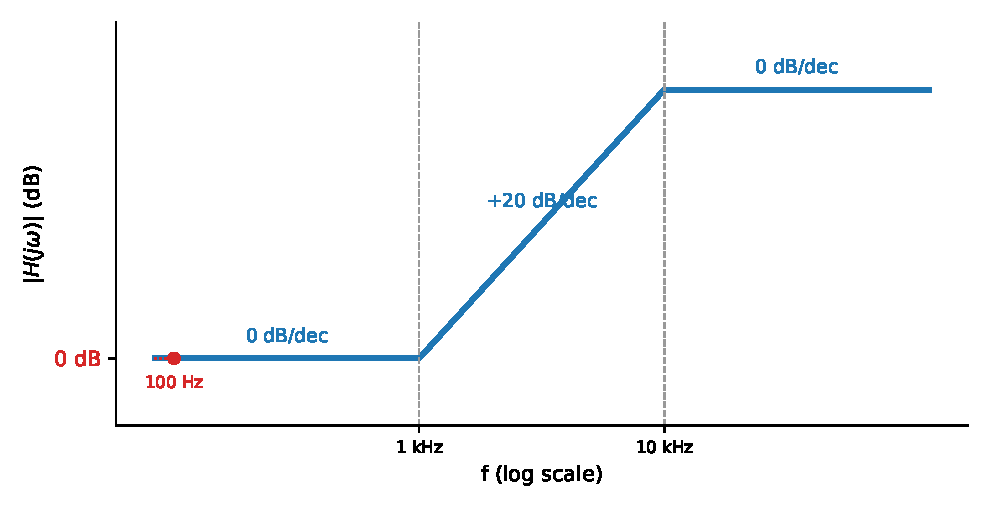
\includegraphics[width=0.7\linewidth,height=5cm,keepaspectratio]{p05_plot}\end{center}
\solstep{1}{Read the corners and slopes}Go left to right along the plot and write down the slope of every straight segment. At each corner frequency the slope changes by a multiple of 20\,dB/dec: every $-20$ is one pole, every $+20$ is one zero (tool T6 read backwards).\begin{center}\renewcommand{\arraystretch}{1.35}
\begin{tabular}{ccccl}
\toprule
corner $f_c$ & slope before & slope after & change & meaning \\
\midrule
1 kHz & $0$ & $+20$ & $+20$ & one zero at $f_c$ \\
10 kHz & $+20$ & $0$ & $-20$ & one pole at $f_c$ \\
\bottomrule
\end{tabular}\end{center}

\solstep{2}{Starting slope $\Rightarrow$ factors of $s$}The plot starts \emph{flat} (0\,dB/dec), so there is no factor $s$ in the numerator: every pole is written as $\frac{1}{1+s/p}$ and every zero as $\left(1+\frac{s}{z}\right)$, which are all $\approx1$ (0\,dB) at low frequency. Every corner is an angular frequency $\omega_c=2\pi f_c$.
\solstep{3}{Assemble $H(s)$}Put one factor per pole/zero in front of an unknown constant $K$:\[
H(s) = K\,\left(1+\dfrac{s}{2\pi\cdot 1\mathrm{k}}\right)\,\dfrac{1}{1+\dfrac{s}{2\pi\cdot 10\mathrm{k}}}
\]

\solstep{4}{Find $K$ from the marked level}The plot marks the level $0$\,dB at $f=$\,100 Hz. On the straight-line plot every factor is either exactly 0\,dB (where it is $\approx1$) or a $\pm20$\,dB/dec line, so evaluate the \emph{asymptote} of each factor at that frequency (the level of a line with slope $\pm20$\,dB/dec is $\pm20\log_{10}(f/f_c)$):\begin{center}\renewcommand{\arraystretch}{1.35}
\begin{tabular}{cccc}
\toprule
factor & $f_c$ & at $f=$\,100 Hz & asymptote (dB) \\
\midrule
$\rule[-1.1em]{0pt}{2.8em}\left(1+\dfrac{s}{2\pi\cdot 1\mathrm{k}}\right)$ & 1 kHz & $f<f_c$: $\approx 1$ & $0$ \\
$\rule[-1.7em]{0pt}{4em}\dfrac{1}{1+\dfrac{s}{2\pi\cdot 10\mathrm{k}}}$ & 10 kHz & $f<f_c$: $\approx 1$ & $0$ \\
\textbf{sum} &  &  & $\mathbf{0}$ \\
\bottomrule
\end{tabular}\end{center}
The dB values of the factors \emph{add} (magnitudes multiply), so\[
20\log_{10}K = 0 - (0) = 0\ \mathrm{dB}\quad\Rightarrow\quad K = 10^{0/20} = 1
\]

So\[
\boxed{H(s) = 1\,\left(1+\dfrac{s}{2\pi\cdot 1\mathrm{k}}\right)\,\dfrac{1}{1+\dfrac{s}{2\pi\cdot 10\mathrm{k}}}}
\]

\solstep{5}{Check}Rebuild the plot from the factors: each factor's straight-line plot (green) is added to get $|H|$ (blue). It must reproduce every slope of the given plot and the marked level.\begin{center}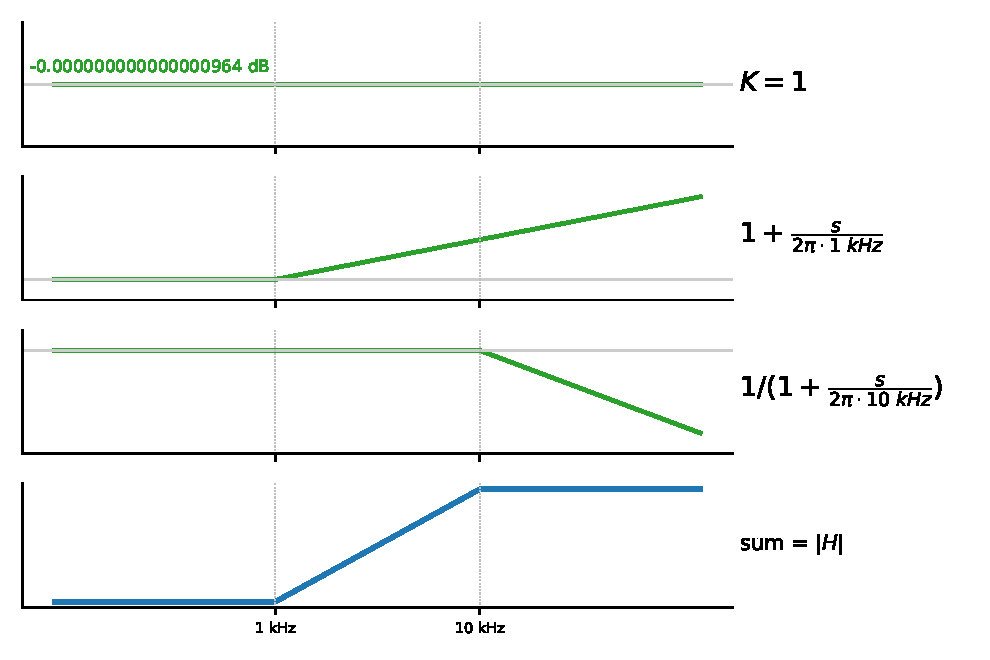
\includegraphics[width=0.82\linewidth,height=9cm,keepaspectratio]{p05_factors}\end{center}
\begin{center}\renewcommand{\arraystretch}{1.35}
\begin{tabular}{lcl}
\toprule
frequency range & slope & asymptote level \\
\midrule
$f<$ 1 kHz & $0$ dB/dec & 0 dB at end \\
1 kHz -- 10 kHz & $+20$ dB/dec & 0 dB at start, 20 dB at end \\
$f>$ 10 kHz & $0$ dB/dec & 20 dB at start \\
\bottomrule
\end{tabular}\end{center}

\solstep{6}{Steady-state output}The input is $V_i(t) = 0.5\sin\left(2\pi\cdot 3000\,t\right)$, so $\omega_{in} = 2\pi\cdot 3000 = 18800$\,rad/s. Put $s=j\omega_{in}$ in each factor (tool T5; use the \emph{exact} factors here, not the straight lines): magnitudes multiply, angles add.
{\small Rules: $\left|\frac{s}{s+p}\right| = \frac{\omega}{\sqrt{\omega^2+p^2}}$, $\angle = \frac{\pi}{2}-\tan^{-1}\frac{\omega}{p}$;\quad $\left|\frac{1}{1+s/p}\right| = \frac{1}{\sqrt{1+(\omega/p)^2}}$, $\angle = -\tan^{-1}\frac{\omega}{p}$;\quad $\left|1+\frac{s}{z}\right| = \sqrt{1+(\omega/z)^2}$, $\angle = \tan^{-1}\frac{\omega}{z}$;\quad a negative $K$ adds $-\pi$.}
\begin{center}\renewcommand{\arraystretch}{1.35}
\begin{tabular}{ccc}
\toprule
factor & magnitude & angle (rad) \\
\midrule
$1$ & $1$ & $0$ \\
$\rule[-1.1em]{0pt}{2.8em}\left(1+\dfrac{s}{2\pi\cdot 1\mathrm{k}}\right)$ & $3.162$ & $1.25$ \\
$\rule[-1.7em]{0pt}{4em}\dfrac{1}{1+\dfrac{s}{2\pi\cdot 10\mathrm{k}}}$ & $0.9578$ & $-0.291$ \\
\textbf{total} & $\mathbf{3.029}$ (product) & $\mathbf{0.958}$ (sum) \\
\bottomrule
\end{tabular}\end{center}

\begin{align*}
|H(j\omega_{in})| &= 3.03, \qquad \angle H(j\omega_{in}) = 0.958\ \mathrm{rad} \\
v_{o,ac}(t) &= 3.03\times 0.5\,\sin\left(2\pi\cdot 3000\,t + 0.958\right) = 1.51\,\sin\left(2\pi\cdot 3000\,t + 0.958\right)
\end{align*}

\[
\boxed{V_o(t) = 1.51\,\sin\left(2\pi\cdot 3000\,t + 0.958\right)\ \mathrm{V}}
\]

\begin{ansbox}
$H(s) = 1\,\left(1+\dfrac{s}{2\pi\cdot 1\mathrm{k}}\right)\,\dfrac{1}{1+\dfrac{s}{2\pi\cdot 10\mathrm{k}}}$\quad (corners: 1 kHz, 10 kHz)\\[4pt]
$V_o(t) = 1.51\,\sin\left(2\pi\cdot 3000\,t + 0.958\right)\ \mathrm{V}$
\end{ansbox}

\newpage
\subsection*{Solution 1D.6 \hfill Easy}
\begin{center}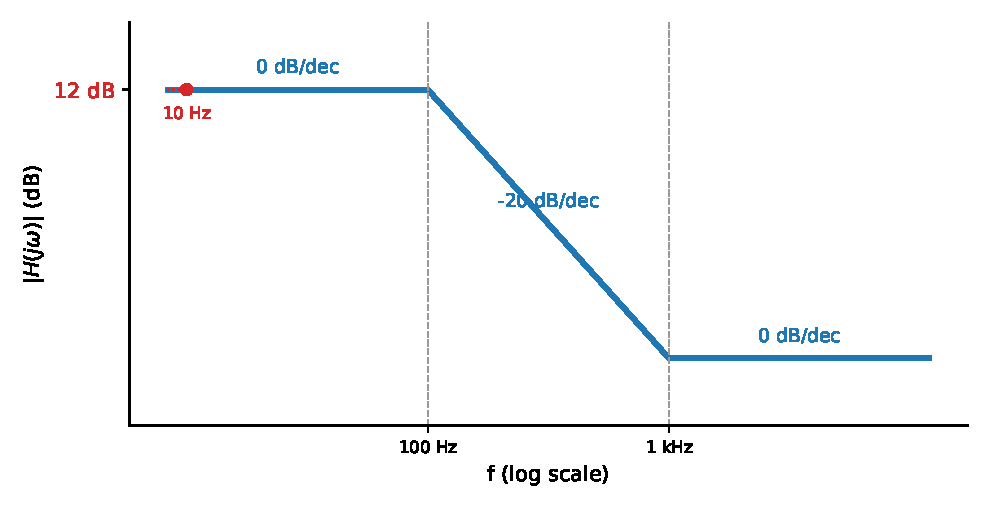
\includegraphics[width=0.7\linewidth,height=5cm,keepaspectratio]{p06_plot}\end{center}
\solstep{1}{Read the corners and slopes}Go left to right along the plot and write down the slope of every straight segment. At each corner frequency the slope changes by a multiple of 20\,dB/dec: every $-20$ is one pole, every $+20$ is one zero (tool T6 read backwards).\begin{center}\renewcommand{\arraystretch}{1.35}
\begin{tabular}{ccccl}
\toprule
corner $f_c$ & slope before & slope after & change & meaning \\
\midrule
100 Hz & $0$ & $-20$ & $-20$ & one pole at $f_c$ \\
1 kHz & $-20$ & $0$ & $+20$ & one zero at $f_c$ \\
\bottomrule
\end{tabular}\end{center}

\solstep{2}{Starting slope $\Rightarrow$ factors of $s$}The plot starts \emph{flat} (0\,dB/dec), so there is no factor $s$ in the numerator: every pole is written as $\frac{1}{1+s/p}$ and every zero as $\left(1+\frac{s}{z}\right)$, which are all $\approx1$ (0\,dB) at low frequency. Every corner is an angular frequency $\omega_c=2\pi f_c$.
\solstep{3}{Assemble $H(s)$}Put one factor per pole/zero in front of an unknown constant $K$:\[
H(s) = K\,\dfrac{1}{1+\dfrac{s}{2\pi\cdot 100}}\,\left(1+\dfrac{s}{2\pi\cdot 1\mathrm{k}}\right)
\]

\solstep{4}{Find $K$ from the marked level}The plot marks the level $12$\,dB at $f=$\,10 Hz. On the straight-line plot every factor is either exactly 0\,dB (where it is $\approx1$) or a $\pm20$\,dB/dec line, so evaluate the \emph{asymptote} of each factor at that frequency (the level of a line with slope $\pm20$\,dB/dec is $\pm20\log_{10}(f/f_c)$):\begin{center}\renewcommand{\arraystretch}{1.35}
\begin{tabular}{cccc}
\toprule
factor & $f_c$ & at $f=$\,10 Hz & asymptote (dB) \\
\midrule
$\rule[-1.7em]{0pt}{4em}\dfrac{1}{1+\dfrac{s}{2\pi\cdot 100}}$ & 100 Hz & $f<f_c$: $\approx 1$ & $0$ \\
$\rule[-1.1em]{0pt}{2.8em}\left(1+\dfrac{s}{2\pi\cdot 1\mathrm{k}}\right)$ & 1 kHz & $f<f_c$: $\approx 1$ & $0$ \\
\textbf{sum} &  &  & $\mathbf{0}$ \\
\bottomrule
\end{tabular}\end{center}
The dB values of the factors \emph{add} (magnitudes multiply), so\[
20\log_{10}K = 12 - (0) = 12\ \mathrm{dB}\quad\Rightarrow\quad K = 10^{12/20} = 3.98
\]

So\[
\boxed{H(s) = 3.98\,\dfrac{1}{1+\dfrac{s}{2\pi\cdot 100}}\,\left(1+\dfrac{s}{2\pi\cdot 1\mathrm{k}}\right)}
\]

\solstep{5}{Check}Rebuild the plot from the factors: each factor's straight-line plot (green) is added to get $|H|$ (blue). It must reproduce every slope of the given plot and the marked level.\begin{center}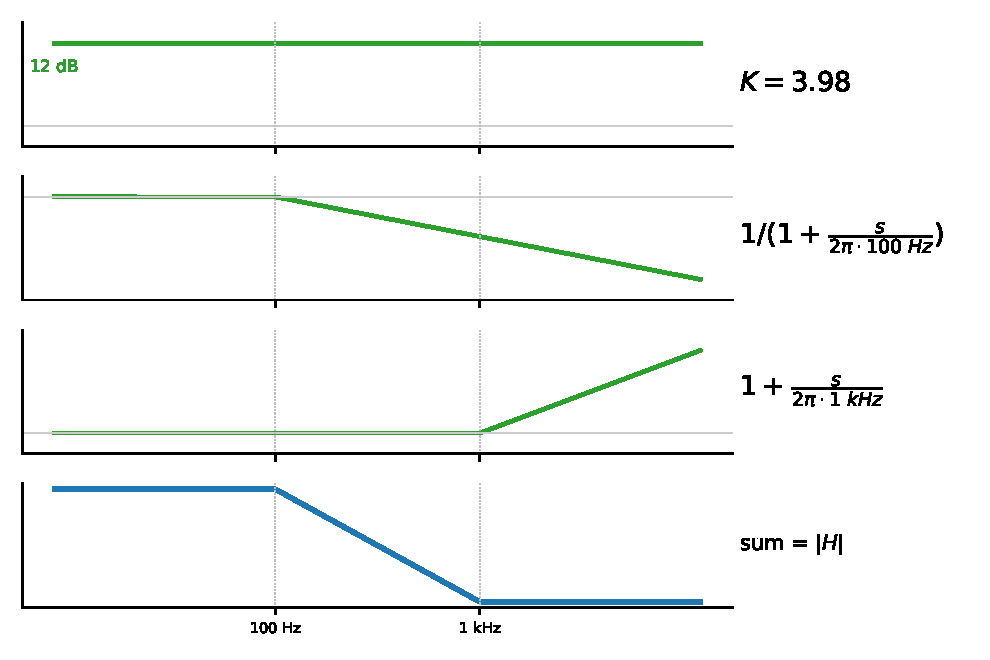
\includegraphics[width=0.82\linewidth,height=9cm,keepaspectratio]{p06_factors}\end{center}
\begin{center}\renewcommand{\arraystretch}{1.35}
\begin{tabular}{lcl}
\toprule
frequency range & slope & asymptote level \\
\midrule
$f<$ 100 Hz & $0$ dB/dec & 12 dB at end \\
100 Hz -- 1 kHz & $-20$ dB/dec & 12 dB at start, -8 dB at end \\
$f>$ 1 kHz & $0$ dB/dec & -8 dB at start \\
\bottomrule
\end{tabular}\end{center}

\solstep{6}{Steady-state output}The input is $V_i(t) = 1\sin\left(2\pi\cdot 500\,t\right)$, so $\omega_{in} = 2\pi\cdot 500 = 3140$\,rad/s. Put $s=j\omega_{in}$ in each factor (tool T5; use the \emph{exact} factors here, not the straight lines): magnitudes multiply, angles add.
{\small Rules: $\left|\frac{s}{s+p}\right| = \frac{\omega}{\sqrt{\omega^2+p^2}}$, $\angle = \frac{\pi}{2}-\tan^{-1}\frac{\omega}{p}$;\quad $\left|\frac{1}{1+s/p}\right| = \frac{1}{\sqrt{1+(\omega/p)^2}}$, $\angle = -\tan^{-1}\frac{\omega}{p}$;\quad $\left|1+\frac{s}{z}\right| = \sqrt{1+(\omega/z)^2}$, $\angle = \tan^{-1}\frac{\omega}{z}$;\quad a negative $K$ adds $-\pi$.}
\begin{center}\renewcommand{\arraystretch}{1.35}
\begin{tabular}{ccc}
\toprule
factor & magnitude & angle (rad) \\
\midrule
$3.98$ & $3.981$ & $0$ \\
$\rule[-1.7em]{0pt}{4em}\dfrac{1}{1+\dfrac{s}{2\pi\cdot 100}}$ & $0.1961$ & $-1.37$ \\
$\rule[-1.1em]{0pt}{2.8em}\left(1+\dfrac{s}{2\pi\cdot 1\mathrm{k}}\right)$ & $1.118$ & $0.464$ \\
\textbf{total} & $\mathbf{0.8729}$ (product) & $\mathbf{-0.91}$ (sum) \\
\bottomrule
\end{tabular}\end{center}

\begin{align*}
|H(j\omega_{in})| &= 0.873, \qquad \angle H(j\omega_{in}) = -0.91\ \mathrm{rad} \\
v_{o,ac}(t) &= 0.873\times 1\,\sin\left(2\pi\cdot 500\,t - 0.91\right) = 0.873\,\sin\left(2\pi\cdot 500\,t - 0.91\right)
\end{align*}

\[
\boxed{V_o(t) = 0.873\,\sin\left(2\pi\cdot 500\,t - 0.91\right)\ \mathrm{V}}
\]

\begin{ansbox}
$H(s) = 3.98\,\dfrac{1}{1+\dfrac{s}{2\pi\cdot 100}}\,\left(1+\dfrac{s}{2\pi\cdot 1\mathrm{k}}\right)$\quad (corners: 100 Hz, 1 kHz)\\[4pt]
$V_o(t) = 0.873\,\sin\left(2\pi\cdot 500\,t - 0.91\right)\ \mathrm{V}$
\end{ansbox}

\newpage
\subsection*{Solution 1D.7 \hfill Medium}
\begin{center}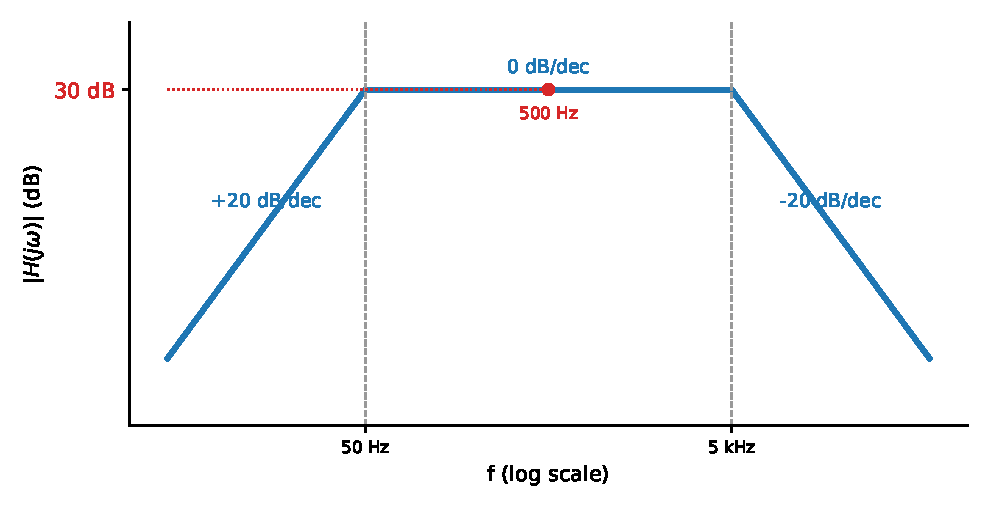
\includegraphics[width=0.7\linewidth,height=5cm,keepaspectratio]{p07_plot}\end{center}
\solstep{1}{Read the corners and slopes}Go left to right along the plot and write down the slope of every straight segment. At each corner frequency the slope changes by a multiple of 20\,dB/dec: every $-20$ is one pole, every $+20$ is one zero (tool T6 read backwards).\begin{center}\renewcommand{\arraystretch}{1.35}
\begin{tabular}{ccccl}
\toprule
corner $f_c$ & slope before & slope after & change & meaning \\
\midrule
50 Hz & $+20$ & $0$ & $-20$ & one pole at $f_c$ \\
5 kHz & $0$ & $-20$ & $-20$ & one pole at $f_c$ \\
\bottomrule
\end{tabular}\end{center}

\solstep{2}{Starting slope $\Rightarrow$ factors of $s$}The plot starts with a slope of $+20$\,dB/dec, i.e. $|H|\propto\omega^1$ at low frequency: the numerator contains $s$. As in class, pair each $s$ with one of the \emph{lowest} poles (50 Hz) as $\frac{s}{s+p}$: such a factor rises at $+20$\,dB/dec below $p$ and is $\approx1$ (0\,dB) above it. The remaining poles are written $\frac{1}{1+s/p}$ and the zeros $\left(1+\frac{s}{z}\right)$. Every corner is an angular frequency $\omega_c=2\pi f_c$.
\solstep{3}{Assemble $H(s)$}Put one factor per pole/zero in front of an unknown constant $K$:\[
H(s) = K\,\dfrac{s}{s+2\pi\cdot 50}\,\dfrac{1}{1+\dfrac{s}{2\pi\cdot 5\mathrm{k}}}
\]

\solstep{4}{Find $K$ from the marked level}The plot marks the level $30$\,dB at $f=$\,500 Hz. On the straight-line plot every factor is either exactly 0\,dB (where it is $\approx1$) or a $\pm20$\,dB/dec line, so evaluate the \emph{asymptote} of each factor at that frequency (the level of a line with slope $\pm20$\,dB/dec is $\pm20\log_{10}(f/f_c)$):\begin{center}\renewcommand{\arraystretch}{1.35}
\begin{tabular}{cccc}
\toprule
factor & $f_c$ & at $f=$\,500 Hz & asymptote (dB) \\
\midrule
$\rule[-1.1em]{0pt}{2.8em}\dfrac{s}{s+2\pi\cdot 50}$ & 50 Hz & $f>f_c$: $\approx 1$ & $0$ \\
$\rule[-1.7em]{0pt}{4em}\dfrac{1}{1+\dfrac{s}{2\pi\cdot 5\mathrm{k}}}$ & 5 kHz & $f<f_c$: $\approx 1$ & $0$ \\
\textbf{sum} &  &  & $\mathbf{0}$ \\
\bottomrule
\end{tabular}\end{center}
The dB values of the factors \emph{add} (magnitudes multiply), so\[
20\log_{10}K = 30 - (0) = 30\ \mathrm{dB}\quad\Rightarrow\quad K = 10^{30/20} = 31.6
\]

So\[
\boxed{H(s) = 31.6\,\dfrac{s}{s+2\pi\cdot 50}\,\dfrac{1}{1+\dfrac{s}{2\pi\cdot 5\mathrm{k}}}}
\]

\solstep{5}{Check}Rebuild the plot from the factors: each factor's straight-line plot (green) is added to get $|H|$ (blue). It must reproduce every slope of the given plot and the marked level.\begin{center}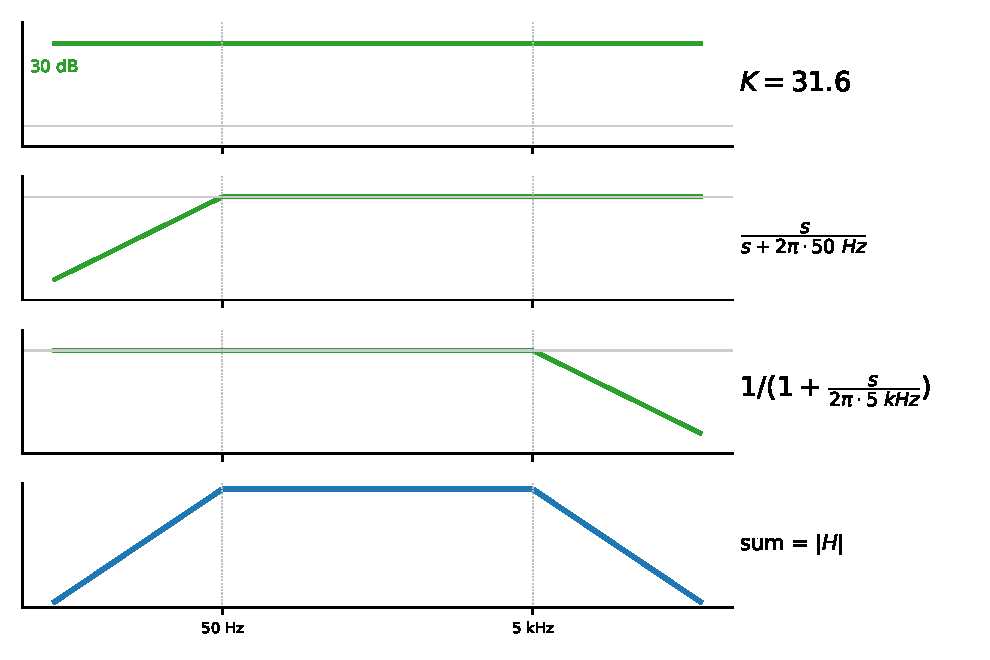
\includegraphics[width=0.82\linewidth,height=9cm,keepaspectratio]{p07_factors}\end{center}
\begin{center}\renewcommand{\arraystretch}{1.35}
\begin{tabular}{lcl}
\toprule
frequency range & slope & asymptote level \\
\midrule
$f<$ 50 Hz & $+20$ dB/dec & 30 dB at end \\
50 Hz -- 5 kHz & $0$ dB/dec & 30 dB at start, 30 dB at end \\
$f>$ 5 kHz & $-20$ dB/dec & 30 dB at start \\
\bottomrule
\end{tabular}\end{center}

\solstep{6}{Steady-state output}The input is $V_i(t) = 0.1\sin\left(2\pi\cdot 20000\,t\right)$, so $\omega_{in} = 2\pi\cdot 20000 = 1.26\times 10^{5}$\,rad/s. Put $s=j\omega_{in}$ in each factor (tool T5; use the \emph{exact} factors here, not the straight lines): magnitudes multiply, angles add.
{\small Rules: $\left|\frac{s}{s+p}\right| = \frac{\omega}{\sqrt{\omega^2+p^2}}$, $\angle = \frac{\pi}{2}-\tan^{-1}\frac{\omega}{p}$;\quad $\left|\frac{1}{1+s/p}\right| = \frac{1}{\sqrt{1+(\omega/p)^2}}$, $\angle = -\tan^{-1}\frac{\omega}{p}$;\quad $\left|1+\frac{s}{z}\right| = \sqrt{1+(\omega/z)^2}$, $\angle = \tan^{-1}\frac{\omega}{z}$;\quad a negative $K$ adds $-\pi$.}
\begin{center}\renewcommand{\arraystretch}{1.35}
\begin{tabular}{ccc}
\toprule
factor & magnitude & angle (rad) \\
\midrule
$31.6$ & $31.62$ & $0$ \\
$\rule[-1.1em]{0pt}{2.8em}\dfrac{s}{s+2\pi\cdot 50}$ & $1$ & $0.0025$ \\
$\rule[-1.7em]{0pt}{4em}\dfrac{1}{1+\dfrac{s}{2\pi\cdot 5\mathrm{k}}}$ & $0.2425$ & $-1.33$ \\
\textbf{total} & $\mathbf{7.67}$ (product) & $\mathbf{-1.32}$ (sum) \\
\bottomrule
\end{tabular}\end{center}

\begin{align*}
|H(j\omega_{in})| &= 7.67, \qquad \angle H(j\omega_{in}) = -1.32\ \mathrm{rad} \\
v_{o,ac}(t) &= 7.67\times 0.1\,\sin\left(2\pi\cdot 20000\,t - 1.32\right) = 0.767\,\sin\left(2\pi\cdot 20000\,t - 1.32\right)
\end{align*}

\[
\boxed{V_o(t) = 0.767\,\sin\left(2\pi\cdot 20000\,t - 1.32\right)\ \mathrm{V}}
\]

\begin{ansbox}
$H(s) = 31.6\,\dfrac{s}{s+2\pi\cdot 50}\,\dfrac{1}{1+\dfrac{s}{2\pi\cdot 5\mathrm{k}}}$\quad (corners: 50 Hz, 5 kHz)\\[4pt]
$V_o(t) = 0.767\,\sin\left(2\pi\cdot 20000\,t - 1.32\right)\ \mathrm{V}$
\end{ansbox}

\newpage
\subsection*{Solution 1D.8 \hfill Medium}
\begin{center}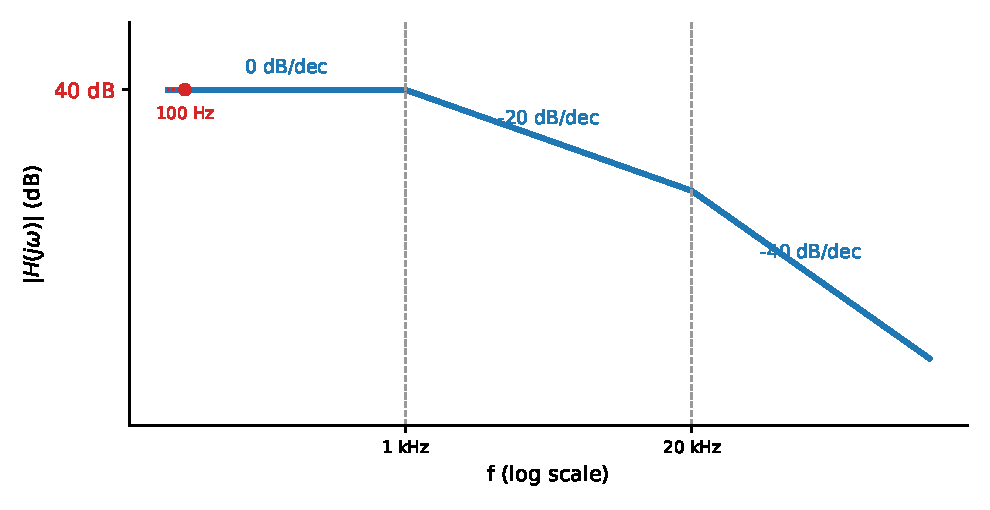
\includegraphics[width=0.7\linewidth,height=5cm,keepaspectratio]{p08_plot}\end{center}
\solstep{1}{Read the corners and slopes}Go left to right along the plot and write down the slope of every straight segment. At each corner frequency the slope changes by a multiple of 20\,dB/dec: every $-20$ is one pole, every $+20$ is one zero (tool T6 read backwards).\begin{center}\renewcommand{\arraystretch}{1.35}
\begin{tabular}{ccccl}
\toprule
corner $f_c$ & slope before & slope after & change & meaning \\
\midrule
1 kHz & $0$ & $-20$ & $-20$ & one pole at $f_c$ \\
20 kHz & $-20$ & $-40$ & $-20$ & one pole at $f_c$ \\
\bottomrule
\end{tabular}\end{center}

\solstep{2}{Starting slope $\Rightarrow$ factors of $s$}The plot starts \emph{flat} (0\,dB/dec), so there is no factor $s$ in the numerator: every pole is written as $\frac{1}{1+s/p}$ and every zero as $\left(1+\frac{s}{z}\right)$, which are all $\approx1$ (0\,dB) at low frequency. Every corner is an angular frequency $\omega_c=2\pi f_c$.
\solstep{3}{Assemble $H(s)$}Put one factor per pole/zero in front of an unknown constant $K$:\[
H(s) = K\,\dfrac{1}{1+\dfrac{s}{2\pi\cdot 1\mathrm{k}}}\,\dfrac{1}{1+\dfrac{s}{2\pi\cdot 20\mathrm{k}}}
\]

\solstep{4}{Find $K$ from the marked level}The plot marks the level $40$\,dB at $f=$\,100 Hz. On the straight-line plot every factor is either exactly 0\,dB (where it is $\approx1$) or a $\pm20$\,dB/dec line, so evaluate the \emph{asymptote} of each factor at that frequency (the level of a line with slope $\pm20$\,dB/dec is $\pm20\log_{10}(f/f_c)$):\begin{center}\renewcommand{\arraystretch}{1.35}
\begin{tabular}{cccc}
\toprule
factor & $f_c$ & at $f=$\,100 Hz & asymptote (dB) \\
\midrule
$\rule[-1.7em]{0pt}{4em}\dfrac{1}{1+\dfrac{s}{2\pi\cdot 1\mathrm{k}}}$ & 1 kHz & $f<f_c$: $\approx 1$ & $0$ \\
$\rule[-1.7em]{0pt}{4em}\dfrac{1}{1+\dfrac{s}{2\pi\cdot 20\mathrm{k}}}$ & 20 kHz & $f<f_c$: $\approx 1$ & $0$ \\
\textbf{sum} &  &  & $\mathbf{0}$ \\
\bottomrule
\end{tabular}\end{center}
The dB values of the factors \emph{add} (magnitudes multiply), so\[
20\log_{10}K = 40 - (0) = 40\ \mathrm{dB}\quad\Rightarrow\quad K = 10^{40/20} = 100
\]

So\[
\boxed{H(s) = 100\,\dfrac{1}{1+\dfrac{s}{2\pi\cdot 1\mathrm{k}}}\,\dfrac{1}{1+\dfrac{s}{2\pi\cdot 20\mathrm{k}}}}
\]

\solstep{5}{Check}Rebuild the plot from the factors: each factor's straight-line plot (green) is added to get $|H|$ (blue). It must reproduce every slope of the given plot and the marked level.\begin{center}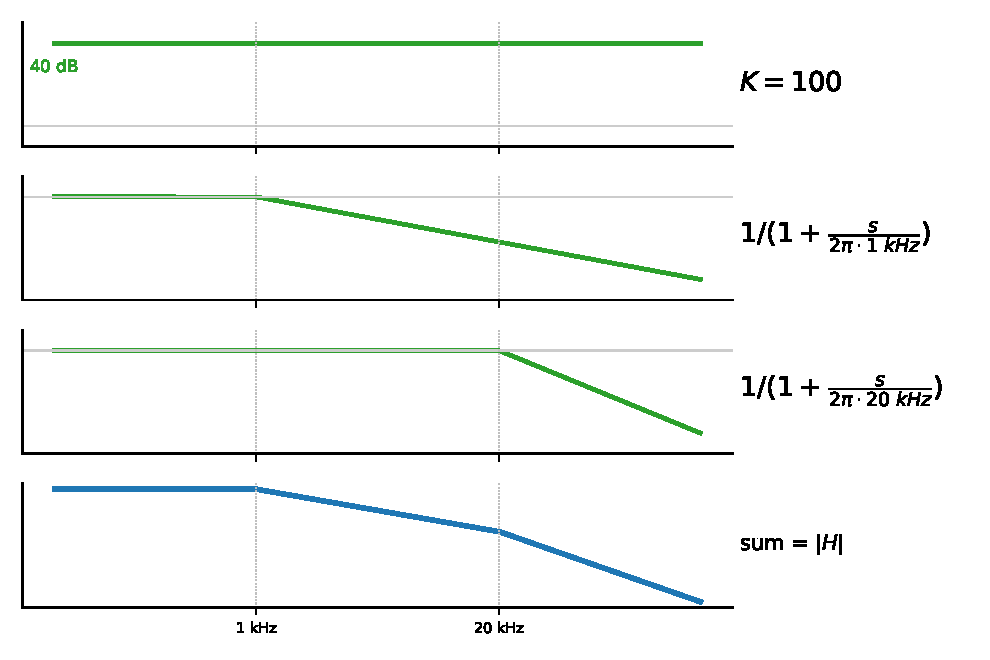
\includegraphics[width=0.82\linewidth,height=9cm,keepaspectratio]{p08_factors}\end{center}
\begin{center}\renewcommand{\arraystretch}{1.35}
\begin{tabular}{lcl}
\toprule
frequency range & slope & asymptote level \\
\midrule
$f<$ 1 kHz & $0$ dB/dec & 40 dB at end \\
1 kHz -- 20 kHz & $-20$ dB/dec & 40 dB at start, 14 dB at end \\
$f>$ 20 kHz & $-40$ dB/dec & 14 dB at start \\
\bottomrule
\end{tabular}\end{center}

\solstep{6}{Steady-state output}The input is $V_i(t) = 0.05\sin\left(2\pi\cdot 5000\,t\right)$, so $\omega_{in} = 2\pi\cdot 5000 = 31400$\,rad/s. Put $s=j\omega_{in}$ in each factor (tool T5; use the \emph{exact} factors here, not the straight lines): magnitudes multiply, angles add.
{\small Rules: $\left|\frac{s}{s+p}\right| = \frac{\omega}{\sqrt{\omega^2+p^2}}$, $\angle = \frac{\pi}{2}-\tan^{-1}\frac{\omega}{p}$;\quad $\left|\frac{1}{1+s/p}\right| = \frac{1}{\sqrt{1+(\omega/p)^2}}$, $\angle = -\tan^{-1}\frac{\omega}{p}$;\quad $\left|1+\frac{s}{z}\right| = \sqrt{1+(\omega/z)^2}$, $\angle = \tan^{-1}\frac{\omega}{z}$;\quad a negative $K$ adds $-\pi$.}
\begin{center}\renewcommand{\arraystretch}{1.35}
\begin{tabular}{ccc}
\toprule
factor & magnitude & angle (rad) \\
\midrule
$100$ & $100$ & $0$ \\
$\rule[-1.7em]{0pt}{4em}\dfrac{1}{1+\dfrac{s}{2\pi\cdot 1\mathrm{k}}}$ & $0.1961$ & $-1.37$ \\
$\rule[-1.7em]{0pt}{4em}\dfrac{1}{1+\dfrac{s}{2\pi\cdot 20\mathrm{k}}}$ & $0.9701$ & $-0.245$ \\
\textbf{total} & $\mathbf{19.03}$ (product) & $\mathbf{-1.62}$ (sum) \\
\bottomrule
\end{tabular}\end{center}

\begin{align*}
|H(j\omega_{in})| &= 19, \qquad \angle H(j\omega_{in}) = -1.62\ \mathrm{rad} \\
v_{o,ac}(t) &= 19\times 0.05\,\sin\left(2\pi\cdot 5000\,t - 1.62\right) = 0.951\,\sin\left(2\pi\cdot 5000\,t - 1.62\right)
\end{align*}

\[
\boxed{V_o(t) = 0.951\,\sin\left(2\pi\cdot 5000\,t - 1.62\right)\ \mathrm{V}}
\]

\begin{ansbox}
$H(s) = 100\,\dfrac{1}{1+\dfrac{s}{2\pi\cdot 1\mathrm{k}}}\,\dfrac{1}{1+\dfrac{s}{2\pi\cdot 20\mathrm{k}}}$\quad (corners: 1 kHz, 20 kHz)\\[4pt]
$V_o(t) = 0.951\,\sin\left(2\pi\cdot 5000\,t - 1.62\right)\ \mathrm{V}$
\end{ansbox}

\newpage
\subsection*{Solution 1D.9 \hfill Medium}
\begin{center}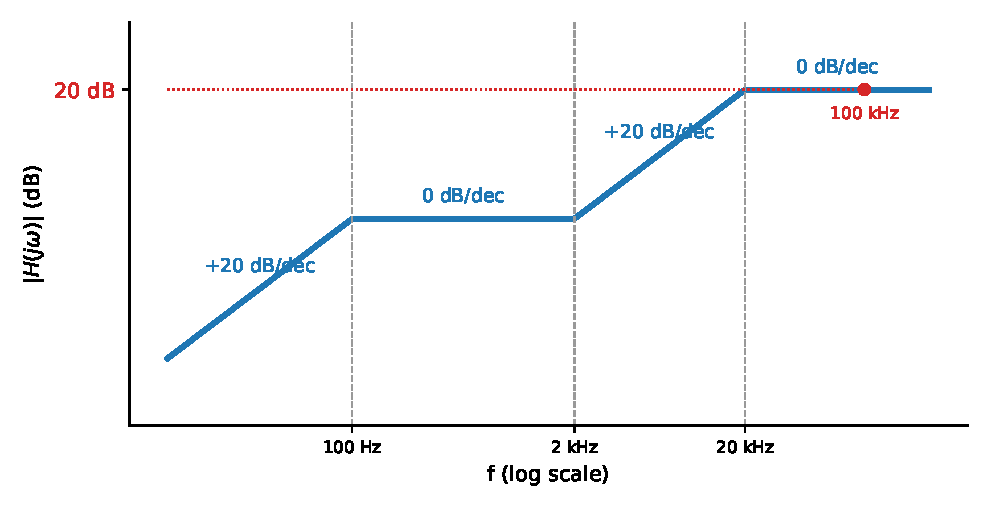
\includegraphics[width=0.7\linewidth,height=5cm,keepaspectratio]{p09_plot}\end{center}
\solstep{1}{Read the corners and slopes}Go left to right along the plot and write down the slope of every straight segment. At each corner frequency the slope changes by a multiple of 20\,dB/dec: every $-20$ is one pole, every $+20$ is one zero (tool T6 read backwards).\begin{center}\renewcommand{\arraystretch}{1.35}
\begin{tabular}{ccccl}
\toprule
corner $f_c$ & slope before & slope after & change & meaning \\
\midrule
100 Hz & $+20$ & $0$ & $-20$ & one pole at $f_c$ \\
2 kHz & $0$ & $+20$ & $+20$ & one zero at $f_c$ \\
20 kHz & $+20$ & $0$ & $-20$ & one pole at $f_c$ \\
\bottomrule
\end{tabular}\end{center}

\solstep{2}{Starting slope $\Rightarrow$ factors of $s$}The plot starts with a slope of $+20$\,dB/dec, i.e. $|H|\propto\omega^1$ at low frequency: the numerator contains $s$. As in class, pair each $s$ with one of the \emph{lowest} poles (100 Hz) as $\frac{s}{s+p}$: such a factor rises at $+20$\,dB/dec below $p$ and is $\approx1$ (0\,dB) above it. The remaining poles are written $\frac{1}{1+s/p}$ and the zeros $\left(1+\frac{s}{z}\right)$. Every corner is an angular frequency $\omega_c=2\pi f_c$.
\solstep{3}{Assemble $H(s)$}Put one factor per pole/zero in front of an unknown constant $K$:\[
H(s) = K\,\dfrac{s}{s+2\pi\cdot 100}\,\left(1+\dfrac{s}{2\pi\cdot 2\mathrm{k}}\right)\,\dfrac{1}{1+\dfrac{s}{2\pi\cdot 20\mathrm{k}}}
\]

\solstep{4}{Find $K$ from the marked level}The plot marks the level $20$\,dB at $f=$\,100 kHz. On the straight-line plot every factor is either exactly 0\,dB (where it is $\approx1$) or a $\pm20$\,dB/dec line, so evaluate the \emph{asymptote} of each factor at that frequency (the level of a line with slope $\pm20$\,dB/dec is $\pm20\log_{10}(f/f_c)$):\begin{center}\renewcommand{\arraystretch}{1.35}
\begin{tabular}{cccc}
\toprule
factor & $f_c$ & at $f=$\,100 kHz & asymptote (dB) \\
\midrule
$\rule[-1.1em]{0pt}{2.8em}\dfrac{s}{s+2\pi\cdot 100}$ & 100 Hz & $f>f_c$: $\approx 1$ & $0$ \\
$\rule[-1.1em]{0pt}{2.8em}\left(1+\dfrac{s}{2\pi\cdot 2\mathrm{k}}\right)$ & 2 kHz & $f>f_c$: $\approx \frac{\omega}{z}$ & $34$ \\
$\rule[-1.7em]{0pt}{4em}\dfrac{1}{1+\dfrac{s}{2\pi\cdot 20\mathrm{k}}}$ & 20 kHz & $f>f_c$: $\approx \frac{p}{\omega}$ & $-14$ \\
\textbf{sum} &  &  & $\mathbf{20}$ \\
\bottomrule
\end{tabular}\end{center}
The dB values of the factors \emph{add} (magnitudes multiply), so\[
20\log_{10}K = 20 - (20) = 0\ \mathrm{dB}\quad\Rightarrow\quad K = 10^{0/20} = 1
\]

So\[
\boxed{H(s) = 1\,\dfrac{s}{s+2\pi\cdot 100}\,\left(1+\dfrac{s}{2\pi\cdot 2\mathrm{k}}\right)\,\dfrac{1}{1+\dfrac{s}{2\pi\cdot 20\mathrm{k}}}}
\]

\solstep{5}{Check}Rebuild the plot from the factors: each factor's straight-line plot (green) is added to get $|H|$ (blue). It must reproduce every slope of the given plot and the marked level.\begin{center}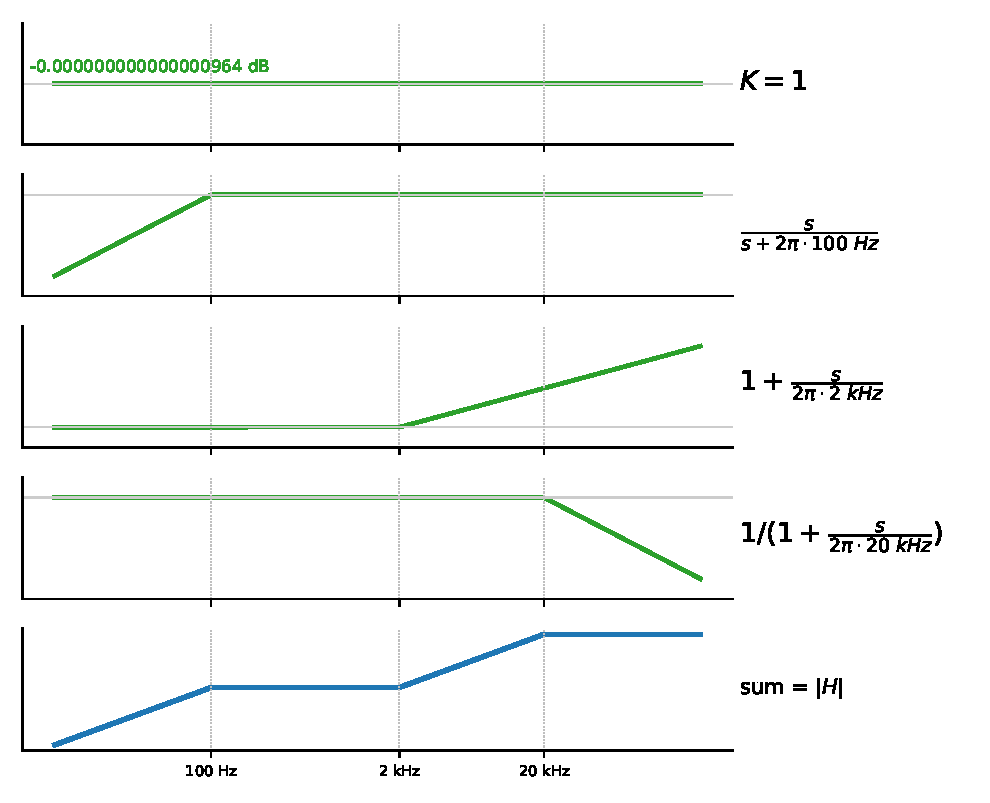
\includegraphics[width=0.82\linewidth,height=9cm,keepaspectratio]{p09_factors}\end{center}
\begin{center}\renewcommand{\arraystretch}{1.35}
\begin{tabular}{lcl}
\toprule
frequency range & slope & asymptote level \\
\midrule
$f<$ 100 Hz & $+20$ dB/dec & 0 dB at end \\
100 Hz -- 2 kHz & $0$ dB/dec & 0 dB at start, 0 dB at end \\
2 kHz -- 20 kHz & $+20$ dB/dec & 0 dB at start, 20 dB at end \\
$f>$ 20 kHz & $0$ dB/dec & 20 dB at start \\
\bottomrule
\end{tabular}\end{center}

\solstep{6}{Steady-state output}The input is $V_i(t) = 0.2\sin\left(2\pi\cdot 1000\,t\right)$, so $\omega_{in} = 2\pi\cdot 1000 = 6280$\,rad/s. Put $s=j\omega_{in}$ in each factor (tool T5; use the \emph{exact} factors here, not the straight lines): magnitudes multiply, angles add.
{\small Rules: $\left|\frac{s}{s+p}\right| = \frac{\omega}{\sqrt{\omega^2+p^2}}$, $\angle = \frac{\pi}{2}-\tan^{-1}\frac{\omega}{p}$;\quad $\left|\frac{1}{1+s/p}\right| = \frac{1}{\sqrt{1+(\omega/p)^2}}$, $\angle = -\tan^{-1}\frac{\omega}{p}$;\quad $\left|1+\frac{s}{z}\right| = \sqrt{1+(\omega/z)^2}$, $\angle = \tan^{-1}\frac{\omega}{z}$;\quad a negative $K$ adds $-\pi$.}
\begin{center}\renewcommand{\arraystretch}{1.35}
\begin{tabular}{ccc}
\toprule
factor & magnitude & angle (rad) \\
\midrule
$1$ & $1$ & $0$ \\
$\rule[-1.1em]{0pt}{2.8em}\dfrac{s}{s+2\pi\cdot 100}$ & $0.995$ & $0.0997$ \\
$\rule[-1.1em]{0pt}{2.8em}\left(1+\dfrac{s}{2\pi\cdot 2\mathrm{k}}\right)$ & $1.118$ & $0.464$ \\
$\rule[-1.7em]{0pt}{4em}\dfrac{1}{1+\dfrac{s}{2\pi\cdot 20\mathrm{k}}}$ & $0.9988$ & $-0.05$ \\
\textbf{total} & $\mathbf{1.111}$ (product) & $\mathbf{0.513}$ (sum) \\
\bottomrule
\end{tabular}\end{center}

\begin{align*}
|H(j\omega_{in})| &= 1.11, \qquad \angle H(j\omega_{in}) = 0.513\ \mathrm{rad} \\
v_{o,ac}(t) &= 1.11\times 0.2\,\sin\left(2\pi\cdot 1000\,t + 0.513\right) = 0.222\,\sin\left(2\pi\cdot 1000\,t + 0.513\right)
\end{align*}

\[
\boxed{V_o(t) = 0.222\,\sin\left(2\pi\cdot 1000\,t + 0.513\right)\ \mathrm{V}}
\]

\begin{ansbox}
$H(s) = 1\,\dfrac{s}{s+2\pi\cdot 100}\,\left(1+\dfrac{s}{2\pi\cdot 2\mathrm{k}}\right)\,\dfrac{1}{1+\dfrac{s}{2\pi\cdot 20\mathrm{k}}}$\quad (corners: 100 Hz, 2 kHz, 20 kHz)\\[4pt]
$V_o(t) = 0.222\,\sin\left(2\pi\cdot 1000\,t + 0.513\right)\ \mathrm{V}$
\end{ansbox}

\newpage
\subsection*{Solution 1D.10 \hfill Medium}
\begin{center}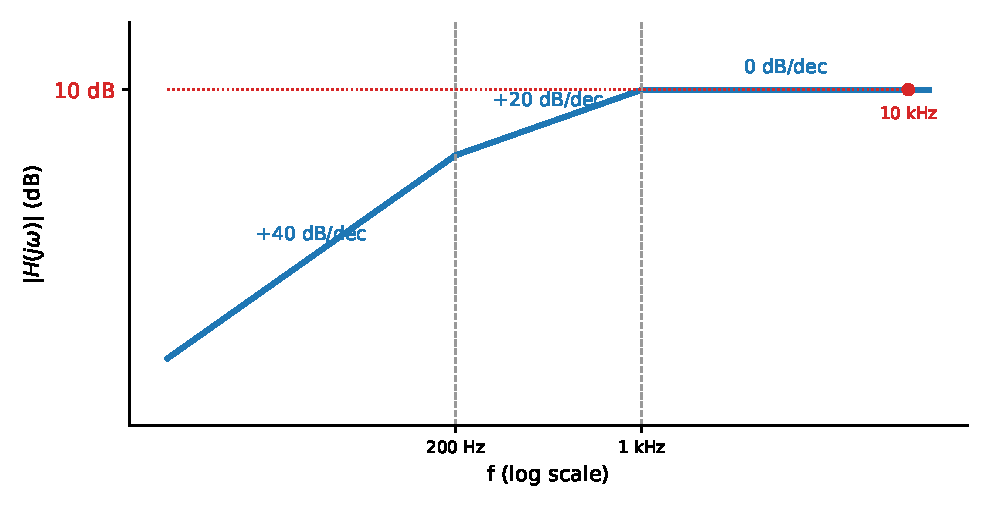
\includegraphics[width=0.7\linewidth,height=5cm,keepaspectratio]{p10_plot}\end{center}
\solstep{1}{Read the corners and slopes}Go left to right along the plot and write down the slope of every straight segment. At each corner frequency the slope changes by a multiple of 20\,dB/dec: every $-20$ is one pole, every $+20$ is one zero (tool T6 read backwards).\begin{center}\renewcommand{\arraystretch}{1.35}
\begin{tabular}{ccccl}
\toprule
corner $f_c$ & slope before & slope after & change & meaning \\
\midrule
200 Hz & $+40$ & $+20$ & $-20$ & one pole at $f_c$ \\
1 kHz & $+20$ & $0$ & $-20$ & one pole at $f_c$ \\
\bottomrule
\end{tabular}\end{center}

\solstep{2}{Starting slope $\Rightarrow$ factors of $s$}The plot starts with a slope of $+40$\,dB/dec, i.e. $|H|\propto\omega^2$ at low frequency: the numerator contains $s^2$. As in class, pair each $s$ with one of the \emph{lowest} poles (200 Hz, 1 kHz) as $\frac{s}{s+p}$: such a factor rises at $+20$\,dB/dec below $p$ and is $\approx1$ (0\,dB) above it. The remaining poles are written $\frac{1}{1+s/p}$ and the zeros $\left(1+\frac{s}{z}\right)$. Every corner is an angular frequency $\omega_c=2\pi f_c$.
\solstep{3}{Assemble $H(s)$}Put one factor per pole/zero in front of an unknown constant $K$:\[
H(s) = K\,\dfrac{s}{s+2\pi\cdot 200}\,\dfrac{s}{s+2\pi\cdot 1\mathrm{k}}
\]

\solstep{4}{Find $K$ from the marked level}The plot marks the level $10$\,dB at $f=$\,10 kHz. On the straight-line plot every factor is either exactly 0\,dB (where it is $\approx1$) or a $\pm20$\,dB/dec line, so evaluate the \emph{asymptote} of each factor at that frequency (the level of a line with slope $\pm20$\,dB/dec is $\pm20\log_{10}(f/f_c)$):\begin{center}\renewcommand{\arraystretch}{1.35}
\begin{tabular}{cccc}
\toprule
factor & $f_c$ & at $f=$\,10 kHz & asymptote (dB) \\
\midrule
$\rule[-1.1em]{0pt}{2.8em}\dfrac{s}{s+2\pi\cdot 200}$ & 200 Hz & $f>f_c$: $\approx 1$ & $0$ \\
$\rule[-1.1em]{0pt}{2.8em}\dfrac{s}{s+2\pi\cdot 1\mathrm{k}}$ & 1 kHz & $f>f_c$: $\approx 1$ & $0$ \\
\textbf{sum} &  &  & $\mathbf{0}$ \\
\bottomrule
\end{tabular}\end{center}
The dB values of the factors \emph{add} (magnitudes multiply), so\[
20\log_{10}K = 10 - (0) = 10\ \mathrm{dB}\quad\Rightarrow\quad K = 10^{10/20} = 3.16
\]

So\[
\boxed{H(s) = 3.16\,\dfrac{s}{s+2\pi\cdot 200}\,\dfrac{s}{s+2\pi\cdot 1\mathrm{k}}}
\]

\solstep{5}{Check}Rebuild the plot from the factors: each factor's straight-line plot (green) is added to get $|H|$ (blue). It must reproduce every slope of the given plot and the marked level.\begin{center}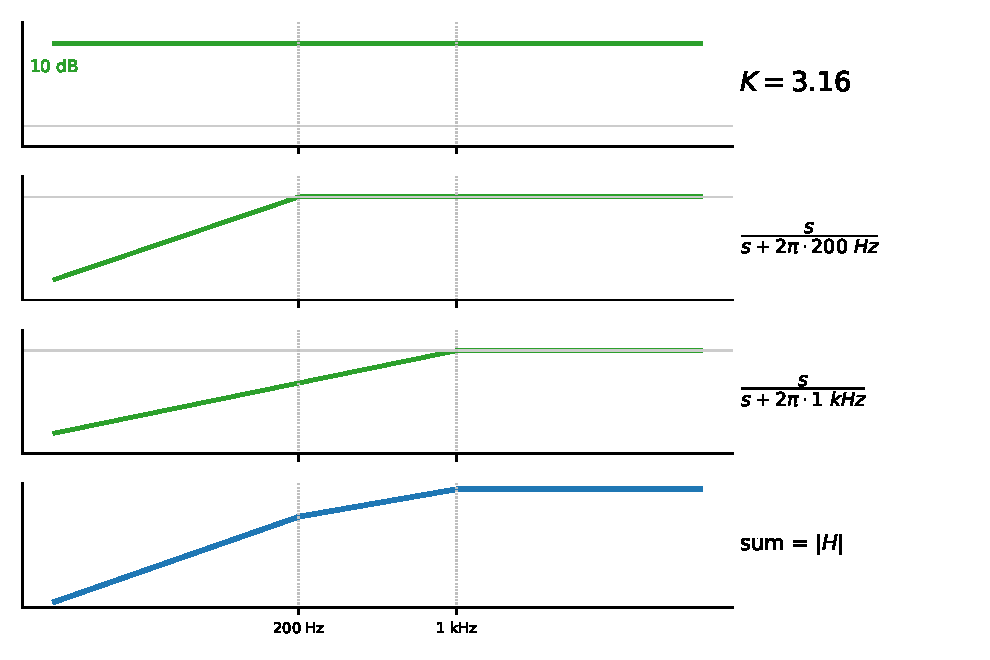
\includegraphics[width=0.82\linewidth,height=9cm,keepaspectratio]{p10_factors}\end{center}
\begin{center}\renewcommand{\arraystretch}{1.35}
\begin{tabular}{lcl}
\toprule
frequency range & slope & asymptote level \\
\midrule
$f<$ 200 Hz & $+40$ dB/dec & -3.98 dB at end \\
200 Hz -- 1 kHz & $+20$ dB/dec & -3.98 dB at start, 10 dB at end \\
$f>$ 1 kHz & $0$ dB/dec & 10 dB at start \\
\bottomrule
\end{tabular}\end{center}

\solstep{6}{Steady-state output}The input is $V_i(t) = 0.5\sin\left(2\pi\cdot 400\,t\right)$, so $\omega_{in} = 2\pi\cdot 400 = 2510$\,rad/s. Put $s=j\omega_{in}$ in each factor (tool T5; use the \emph{exact} factors here, not the straight lines): magnitudes multiply, angles add.
{\small Rules: $\left|\frac{s}{s+p}\right| = \frac{\omega}{\sqrt{\omega^2+p^2}}$, $\angle = \frac{\pi}{2}-\tan^{-1}\frac{\omega}{p}$;\quad $\left|\frac{1}{1+s/p}\right| = \frac{1}{\sqrt{1+(\omega/p)^2}}$, $\angle = -\tan^{-1}\frac{\omega}{p}$;\quad $\left|1+\frac{s}{z}\right| = \sqrt{1+(\omega/z)^2}$, $\angle = \tan^{-1}\frac{\omega}{z}$;\quad a negative $K$ adds $-\pi$.}
\begin{center}\renewcommand{\arraystretch}{1.35}
\begin{tabular}{ccc}
\toprule
factor & magnitude & angle (rad) \\
\midrule
$3.16$ & $3.162$ & $0$ \\
$\rule[-1.1em]{0pt}{2.8em}\dfrac{s}{s+2\pi\cdot 200}$ & $0.8944$ & $0.464$ \\
$\rule[-1.1em]{0pt}{2.8em}\dfrac{s}{s+2\pi\cdot 1\mathrm{k}}$ & $0.3714$ & $1.19$ \\
\textbf{total} & $\mathbf{1.05}$ (product) & $\mathbf{1.65}$ (sum) \\
\bottomrule
\end{tabular}\end{center}

\begin{align*}
|H(j\omega_{in})| &= 1.05, \qquad \angle H(j\omega_{in}) = 1.65\ \mathrm{rad} \\
v_{o,ac}(t) &= 1.05\times 0.5\,\sin\left(2\pi\cdot 400\,t + 1.65\right) = 0.525\,\sin\left(2\pi\cdot 400\,t + 1.65\right)
\end{align*}

\[
\boxed{V_o(t) = 0.525\,\sin\left(2\pi\cdot 400\,t + 1.65\right)\ \mathrm{V}}
\]

\begin{ansbox}
$H(s) = 3.16\,\dfrac{s}{s+2\pi\cdot 200}\,\dfrac{s}{s+2\pi\cdot 1\mathrm{k}}$\quad (corners: 200 Hz, 1 kHz)\\[4pt]
$V_o(t) = 0.525\,\sin\left(2\pi\cdot 400\,t + 1.65\right)\ \mathrm{V}$
\end{ansbox}

\newpage
\subsection*{Solution 1D.11 \hfill Medium}
\begin{center}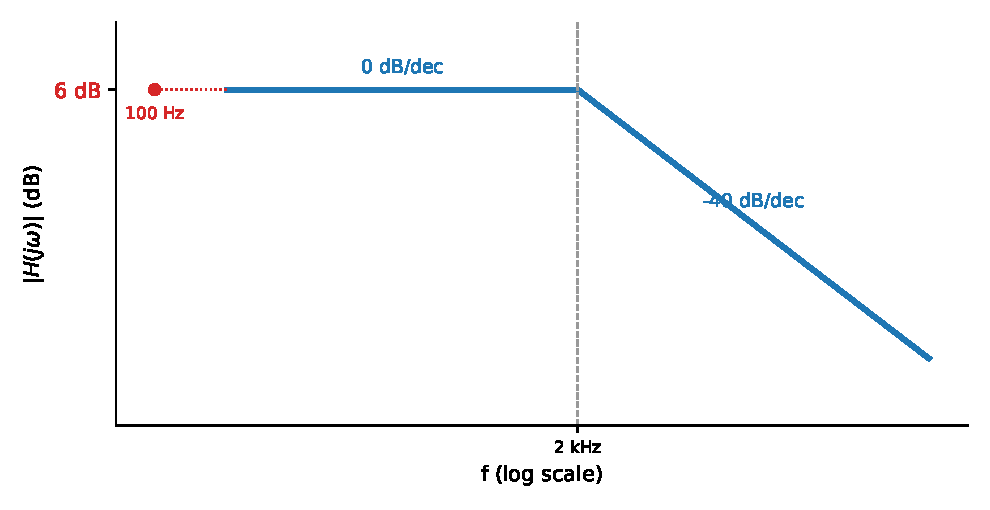
\includegraphics[width=0.7\linewidth,height=5cm,keepaspectratio]{p11_plot}\end{center}
\solstep{1}{Read the corners and slopes}Go left to right along the plot and write down the slope of every straight segment. At each corner frequency the slope changes by a multiple of 20\,dB/dec: every $-20$ is one pole, every $+20$ is one zero (tool T6 read backwards).\begin{center}\renewcommand{\arraystretch}{1.35}
\begin{tabular}{ccccl}
\toprule
corner $f_c$ & slope before & slope after & change & meaning \\
\midrule
2 kHz & $0$ & $-40$ & $-40$ & two poles at $f_c$ \\
\bottomrule
\end{tabular}\end{center}

\solstep{2}{Starting slope $\Rightarrow$ factors of $s$}The plot starts \emph{flat} (0\,dB/dec), so there is no factor $s$ in the numerator: every pole is written as $\frac{1}{1+s/p}$ and every zero as $\left(1+\frac{s}{z}\right)$, which are all $\approx1$ (0\,dB) at low frequency. Every corner is an angular frequency $\omega_c=2\pi f_c$.
\solstep{3}{Assemble $H(s)$}Put one factor per pole/zero in front of an unknown constant $K$:\[
H(s) = K\,\dfrac{1}{1+\dfrac{s}{2\pi\cdot 2\mathrm{k}}}\,\dfrac{1}{1+\dfrac{s}{2\pi\cdot 2\mathrm{k}}}
\]

\solstep{4}{Find $K$ from the marked level}The plot marks the level $6$\,dB at $f=$\,100 Hz. On the straight-line plot every factor is either exactly 0\,dB (where it is $\approx1$) or a $\pm20$\,dB/dec line, so evaluate the \emph{asymptote} of each factor at that frequency (the level of a line with slope $\pm20$\,dB/dec is $\pm20\log_{10}(f/f_c)$):\begin{center}\renewcommand{\arraystretch}{1.35}
\begin{tabular}{cccc}
\toprule
factor & $f_c$ & at $f=$\,100 Hz & asymptote (dB) \\
\midrule
$\rule[-1.7em]{0pt}{4em}\dfrac{1}{1+\dfrac{s}{2\pi\cdot 2\mathrm{k}}}$ & 2 kHz & $f<f_c$: $\approx 1$ & $0$ \\
$\rule[-1.7em]{0pt}{4em}\dfrac{1}{1+\dfrac{s}{2\pi\cdot 2\mathrm{k}}}$ & 2 kHz & $f<f_c$: $\approx 1$ & $0$ \\
\textbf{sum} &  &  & $\mathbf{0}$ \\
\bottomrule
\end{tabular}\end{center}
The dB values of the factors \emph{add} (magnitudes multiply), so\[
20\log_{10}K = 6 - (0) = 6\ \mathrm{dB}\quad\Rightarrow\quad K = 10^{6/20} = 2
\]

So\[
\boxed{H(s) = 2\,\dfrac{1}{1+\dfrac{s}{2\pi\cdot 2\mathrm{k}}}\,\dfrac{1}{1+\dfrac{s}{2\pi\cdot 2\mathrm{k}}}}
\]

\solstep{5}{Check}Rebuild the plot from the factors: each factor's straight-line plot (green) is added to get $|H|$ (blue). It must reproduce every slope of the given plot and the marked level.\begin{center}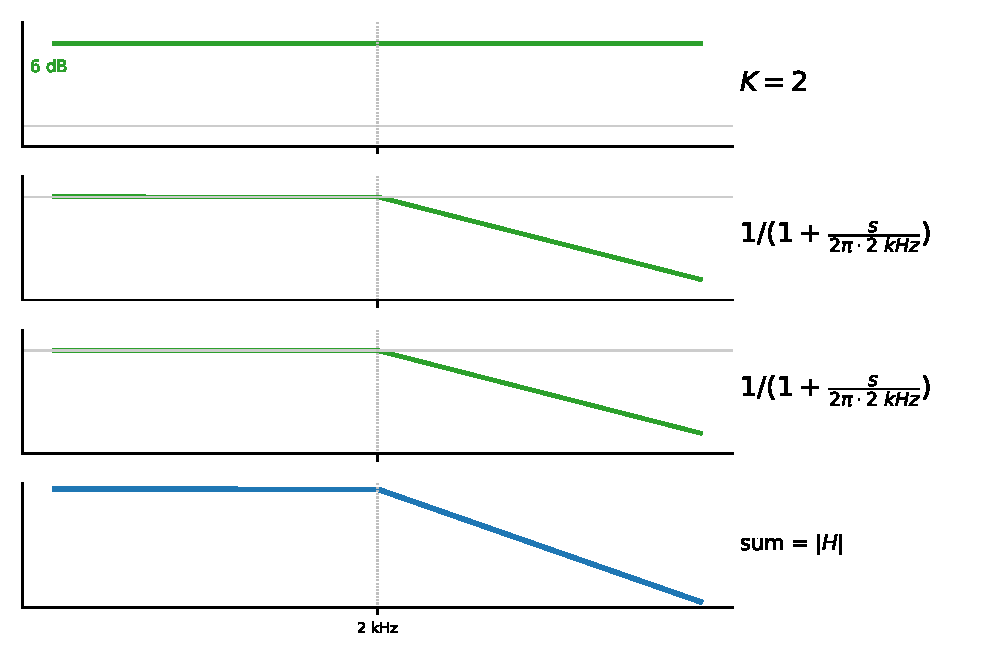
\includegraphics[width=0.82\linewidth,height=9cm,keepaspectratio]{p11_factors}\end{center}
\begin{center}\renewcommand{\arraystretch}{1.35}
\begin{tabular}{lcl}
\toprule
frequency range & slope & asymptote level \\
\midrule
$f<$ 2 kHz & $0$ dB/dec & 6 dB at end \\
$f>$ 2 kHz & $-40$ dB/dec & 6 dB at start \\
\bottomrule
\end{tabular}\end{center}

\solstep{6}{Steady-state output}The input is $V_i(t) = 1\sin\left(2\pi\cdot 4000\,t\right)$, so $\omega_{in} = 2\pi\cdot 4000 = 25100$\,rad/s. Put $s=j\omega_{in}$ in each factor (tool T5; use the \emph{exact} factors here, not the straight lines): magnitudes multiply, angles add.
{\small Rules: $\left|\frac{s}{s+p}\right| = \frac{\omega}{\sqrt{\omega^2+p^2}}$, $\angle = \frac{\pi}{2}-\tan^{-1}\frac{\omega}{p}$;\quad $\left|\frac{1}{1+s/p}\right| = \frac{1}{\sqrt{1+(\omega/p)^2}}$, $\angle = -\tan^{-1}\frac{\omega}{p}$;\quad $\left|1+\frac{s}{z}\right| = \sqrt{1+(\omega/z)^2}$, $\angle = \tan^{-1}\frac{\omega}{z}$;\quad a negative $K$ adds $-\pi$.}
\begin{center}\renewcommand{\arraystretch}{1.35}
\begin{tabular}{ccc}
\toprule
factor & magnitude & angle (rad) \\
\midrule
$2$ & $1.995$ & $0$ \\
$\rule[-1.7em]{0pt}{4em}\dfrac{1}{1+\dfrac{s}{2\pi\cdot 2\mathrm{k}}}$ & $0.4472$ & $-1.11$ \\
$\rule[-1.7em]{0pt}{4em}\dfrac{1}{1+\dfrac{s}{2\pi\cdot 2\mathrm{k}}}$ & $0.4472$ & $-1.11$ \\
\textbf{total} & $\mathbf{0.3991}$ (product) & $\mathbf{-2.21}$ (sum) \\
\bottomrule
\end{tabular}\end{center}

\begin{align*}
|H(j\omega_{in})| &= 0.399, \qquad \angle H(j\omega_{in}) = -2.21\ \mathrm{rad} \\
v_{o,ac}(t) &= 0.399\times 1\,\sin\left(2\pi\cdot 4000\,t - 2.21\right) = 0.399\,\sin\left(2\pi\cdot 4000\,t - 2.21\right)
\end{align*}

\[
\boxed{V_o(t) = 0.399\,\sin\left(2\pi\cdot 4000\,t - 2.21\right)\ \mathrm{V}}
\]

\begin{ansbox}
$H(s) = 2\,\dfrac{1}{1+\dfrac{s}{2\pi\cdot 2\mathrm{k}}}\,\dfrac{1}{1+\dfrac{s}{2\pi\cdot 2\mathrm{k}}}$\quad (corners: 2 kHz, 2 kHz)\\[4pt]
$V_o(t) = 0.399\,\sin\left(2\pi\cdot 4000\,t - 2.21\right)\ \mathrm{V}$
\end{ansbox}

\newpage
\subsection*{Solution 1D.12 \hfill Medium}
\begin{center}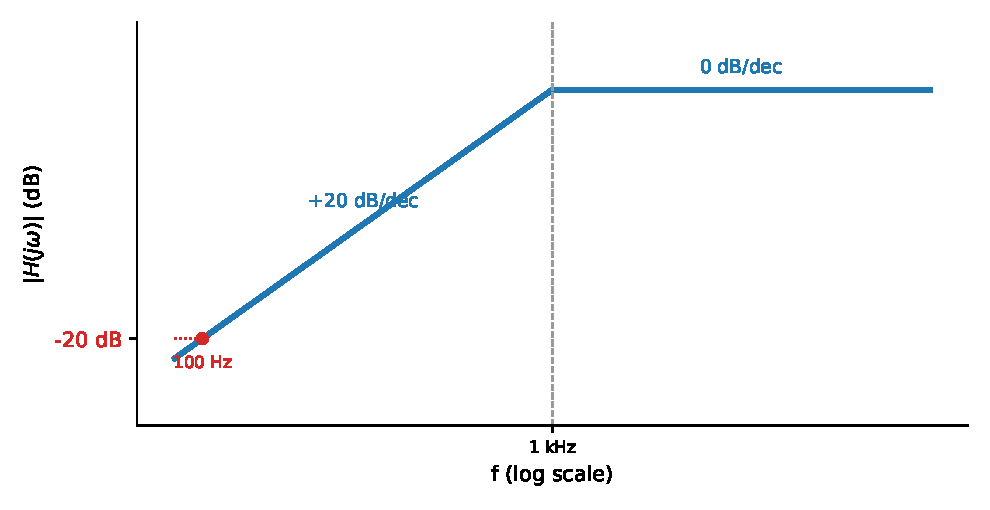
\includegraphics[width=0.7\linewidth,height=5cm,keepaspectratio]{p12_plot}\end{center}
\solstep{1}{Read the corners and slopes}Go left to right along the plot and write down the slope of every straight segment. At each corner frequency the slope changes by a multiple of 20\,dB/dec: every $-20$ is one pole, every $+20$ is one zero (tool T6 read backwards).\begin{center}\renewcommand{\arraystretch}{1.35}
\begin{tabular}{ccccl}
\toprule
corner $f_c$ & slope before & slope after & change & meaning \\
\midrule
1 kHz & $+20$ & $0$ & $-20$ & one pole at $f_c$ \\
\bottomrule
\end{tabular}\end{center}

\solstep{2}{Starting slope $\Rightarrow$ factors of $s$}The plot starts with a slope of $+20$\,dB/dec, i.e. $|H|\propto\omega^1$ at low frequency: the numerator contains $s$. As in class, pair each $s$ with one of the \emph{lowest} poles (1 kHz) as $\frac{s}{s+p}$: such a factor rises at $+20$\,dB/dec below $p$ and is $\approx1$ (0\,dB) above it. The remaining poles are written $\frac{1}{1+s/p}$ and the zeros $\left(1+\frac{s}{z}\right)$. Every corner is an angular frequency $\omega_c=2\pi f_c$.
\solstep{3}{Assemble $H(s)$}Put one factor per pole/zero in front of an unknown constant $K$:\[
H(s) = K\,\dfrac{s}{s+2\pi\cdot 1\mathrm{k}}
\]

\solstep{4}{Find $K$ from the marked level}The plot marks the level $-20$\,dB at $f=$\,100 Hz. On the straight-line plot every factor is either exactly 0\,dB (where it is $\approx1$) or a $\pm20$\,dB/dec line, so evaluate the \emph{asymptote} of each factor at that frequency (the level of a line with slope $\pm20$\,dB/dec is $\pm20\log_{10}(f/f_c)$):\begin{center}\renewcommand{\arraystretch}{1.35}
\begin{tabular}{cccc}
\toprule
factor & $f_c$ & at $f=$\,100 Hz & asymptote (dB) \\
\midrule
$\rule[-1.1em]{0pt}{2.8em}\dfrac{s}{s+2\pi\cdot 1\mathrm{k}}$ & 1 kHz & $f<f_c$: $\approx \frac{\omega}{p}$ & $-20$ \\
\textbf{sum} &  &  & $\mathbf{-20}$ \\
\bottomrule
\end{tabular}\end{center}
The dB values of the factors \emph{add} (magnitudes multiply), so\[
20\log_{10}K = -20 - (-20) = 0\ \mathrm{dB}\quad\Rightarrow\quad K = 10^{0/20} = 1
\]

So\[
\boxed{H(s) = 1\,\dfrac{s}{s+2\pi\cdot 1\mathrm{k}}}
\]

\solstep{5}{Check}Rebuild the plot from the factors: each factor's straight-line plot (green) is added to get $|H|$ (blue). It must reproduce every slope of the given plot and the marked level.\begin{center}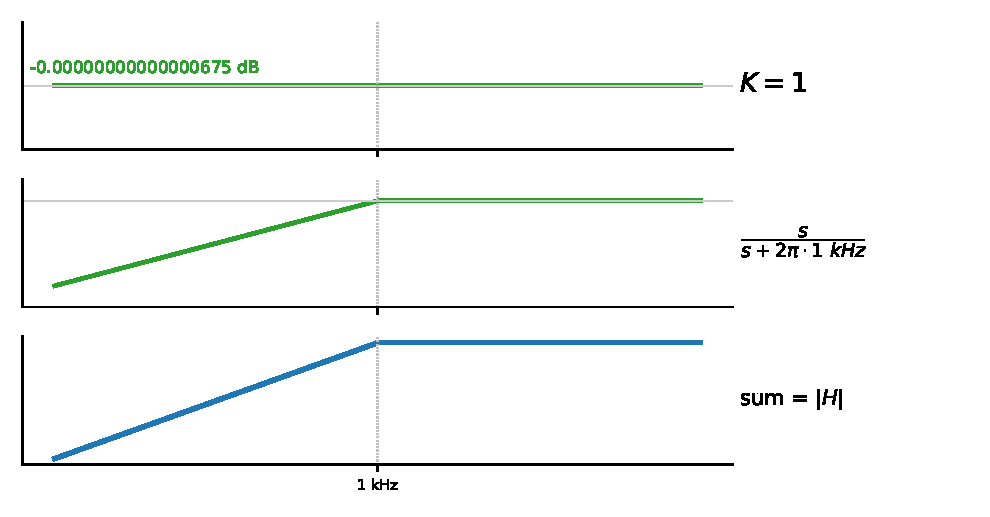
\includegraphics[width=0.82\linewidth,height=9cm,keepaspectratio]{p12_factors}\end{center}
\begin{center}\renewcommand{\arraystretch}{1.35}
\begin{tabular}{lcl}
\toprule
frequency range & slope & asymptote level \\
\midrule
$f<$ 1 kHz & $+20$ dB/dec & 0 dB at end \\
$f>$ 1 kHz & $0$ dB/dec & 0 dB at start \\
\bottomrule
\end{tabular}\end{center}

\solstep{6}{Steady-state output}The input is $V_i(t) = 1\sin\left(2\pi\cdot 2000\,t+\frac{\pi}{4}\right)$, so $\omega_{in} = 2\pi\cdot 2000 = 12600$\,rad/s. Put $s=j\omega_{in}$ in each factor (tool T5; use the \emph{exact} factors here, not the straight lines): magnitudes multiply, angles add.
{\small Rules: $\left|\frac{s}{s+p}\right| = \frac{\omega}{\sqrt{\omega^2+p^2}}$, $\angle = \frac{\pi}{2}-\tan^{-1}\frac{\omega}{p}$;\quad $\left|\frac{1}{1+s/p}\right| = \frac{1}{\sqrt{1+(\omega/p)^2}}$, $\angle = -\tan^{-1}\frac{\omega}{p}$;\quad $\left|1+\frac{s}{z}\right| = \sqrt{1+(\omega/z)^2}$, $\angle = \tan^{-1}\frac{\omega}{z}$;\quad a negative $K$ adds $-\pi$.}
\begin{center}\renewcommand{\arraystretch}{1.35}
\begin{tabular}{ccc}
\toprule
factor & magnitude & angle (rad) \\
\midrule
$1$ & $1$ & $0$ \\
$\rule[-1.1em]{0pt}{2.8em}\dfrac{s}{s+2\pi\cdot 1\mathrm{k}}$ & $0.8944$ & $0.464$ \\
\textbf{total} & $\mathbf{0.8944}$ (product) & $\mathbf{0.464}$ (sum) \\
\bottomrule
\end{tabular}\end{center}

\begin{align*}
|H(j\omega_{in})| &= 0.894, \qquad \angle H(j\omega_{in}) = 0.464\ \mathrm{rad} \\
v_{o,ac}(t) &= 0.894\times 1\,\sin\left(2\pi\cdot 2000\,t + 1.25\right) = 0.894\,\sin\left(2\pi\cdot 2000\,t + 1.25\right)
\end{align*}

(phase: $\theta + \angle H = \frac{\pi}{4} + (0.464) = 1.25$\,rad.)
\[
\boxed{V_o(t) = 0.894\,\sin\left(2\pi\cdot 2000\,t + 1.25\right)\ \mathrm{V}}
\]

\begin{ansbox}
$H(s) = 1\,\dfrac{s}{s+2\pi\cdot 1\mathrm{k}}$\quad (corners: 1 kHz)\\[4pt]
$V_o(t) = 0.894\,\sin\left(2\pi\cdot 2000\,t + 1.25\right)\ \mathrm{V}$
\end{ansbox}

\newpage
\subsection*{Solution 1D.13 \hfill Hard}
\begin{center}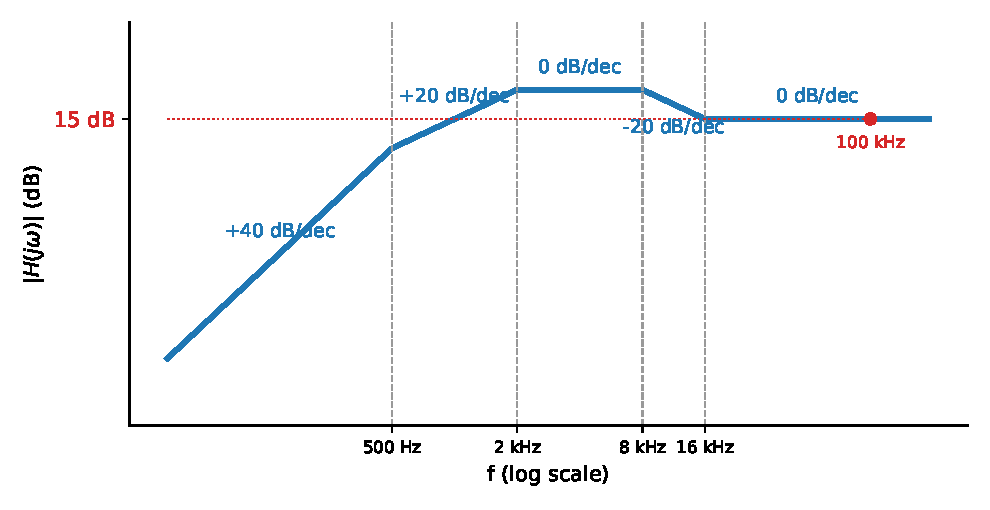
\includegraphics[width=0.7\linewidth,height=5cm,keepaspectratio]{p13_plot}\end{center}
\solstep{1}{Read the corners and slopes}Go left to right along the plot and write down the slope of every straight segment. At each corner frequency the slope changes by a multiple of 20\,dB/dec: every $-20$ is one pole, every $+20$ is one zero (tool T6 read backwards).\begin{center}\renewcommand{\arraystretch}{1.35}
\begin{tabular}{ccccl}
\toprule
corner $f_c$ & slope before & slope after & change & meaning \\
\midrule
500 Hz & $+40$ & $+20$ & $-20$ & one pole at $f_c$ \\
2 kHz & $+20$ & $0$ & $-20$ & one pole at $f_c$ \\
8 kHz & $0$ & $-20$ & $-20$ & one pole at $f_c$ \\
16 kHz & $-20$ & $0$ & $+20$ & one zero at $f_c$ \\
\bottomrule
\end{tabular}\end{center}

\solstep{2}{Starting slope $\Rightarrow$ factors of $s$}The plot starts with a slope of $+40$\,dB/dec, i.e. $|H|\propto\omega^2$ at low frequency: the numerator contains $s^2$. As in class, pair each $s$ with one of the \emph{lowest} poles (500 Hz, 2 kHz) as $\frac{s}{s+p}$: such a factor rises at $+20$\,dB/dec below $p$ and is $\approx1$ (0\,dB) above it. The remaining poles are written $\frac{1}{1+s/p}$ and the zeros $\left(1+\frac{s}{z}\right)$. Every corner is an angular frequency $\omega_c=2\pi f_c$.
\solstep{3}{Assemble $H(s)$}Put one factor per pole/zero in front of an unknown constant $K$:\[
H(s) = K\,\dfrac{s}{s+2\pi\cdot 500}\,\dfrac{s}{s+2\pi\cdot 2\mathrm{k}}\,\dfrac{1}{1+\dfrac{s}{2\pi\cdot 8\mathrm{k}}}\,\left(1+\dfrac{s}{2\pi\cdot 16\mathrm{k}}\right)
\]

\solstep{4}{Find $K$ from the marked level}The plot marks the level $15$\,dB at $f=$\,100 kHz. On the straight-line plot every factor is either exactly 0\,dB (where it is $\approx1$) or a $\pm20$\,dB/dec line, so evaluate the \emph{asymptote} of each factor at that frequency (the level of a line with slope $\pm20$\,dB/dec is $\pm20\log_{10}(f/f_c)$):\begin{center}\renewcommand{\arraystretch}{1.35}
\begin{tabular}{cccc}
\toprule
factor & $f_c$ & at $f=$\,100 kHz & asymptote (dB) \\
\midrule
$\rule[-1.1em]{0pt}{2.8em}\dfrac{s}{s+2\pi\cdot 500}$ & 500 Hz & $f>f_c$: $\approx 1$ & $0$ \\
$\rule[-1.1em]{0pt}{2.8em}\dfrac{s}{s+2\pi\cdot 2\mathrm{k}}$ & 2 kHz & $f>f_c$: $\approx 1$ & $0$ \\
$\rule[-1.7em]{0pt}{4em}\dfrac{1}{1+\dfrac{s}{2\pi\cdot 8\mathrm{k}}}$ & 8 kHz & $f>f_c$: $\approx \frac{p}{\omega}$ & $-21.9$ \\
$\rule[-1.1em]{0pt}{2.8em}\left(1+\dfrac{s}{2\pi\cdot 16\mathrm{k}}\right)$ & 16 kHz & $f>f_c$: $\approx \frac{\omega}{z}$ & $15.9$ \\
\textbf{sum} &  &  & $\mathbf{-6.02}$ \\
\bottomrule
\end{tabular}\end{center}
The dB values of the factors \emph{add} (magnitudes multiply), so\[
20\log_{10}K = 15 - (-6.02) = 21\ \mathrm{dB}\quad\Rightarrow\quad K = 10^{21/20} = 11.2
\]

So\[
\boxed{H(s) = 11.2\,\dfrac{s}{s+2\pi\cdot 500}\,\dfrac{s}{s+2\pi\cdot 2\mathrm{k}}\,\dfrac{1}{1+\dfrac{s}{2\pi\cdot 8\mathrm{k}}}\,\left(1+\dfrac{s}{2\pi\cdot 16\mathrm{k}}\right)}
\]

\solstep{5}{Check}Rebuild the plot from the factors: each factor's straight-line plot (green) is added to get $|H|$ (blue). It must reproduce every slope of the given plot and the marked level.\begin{center}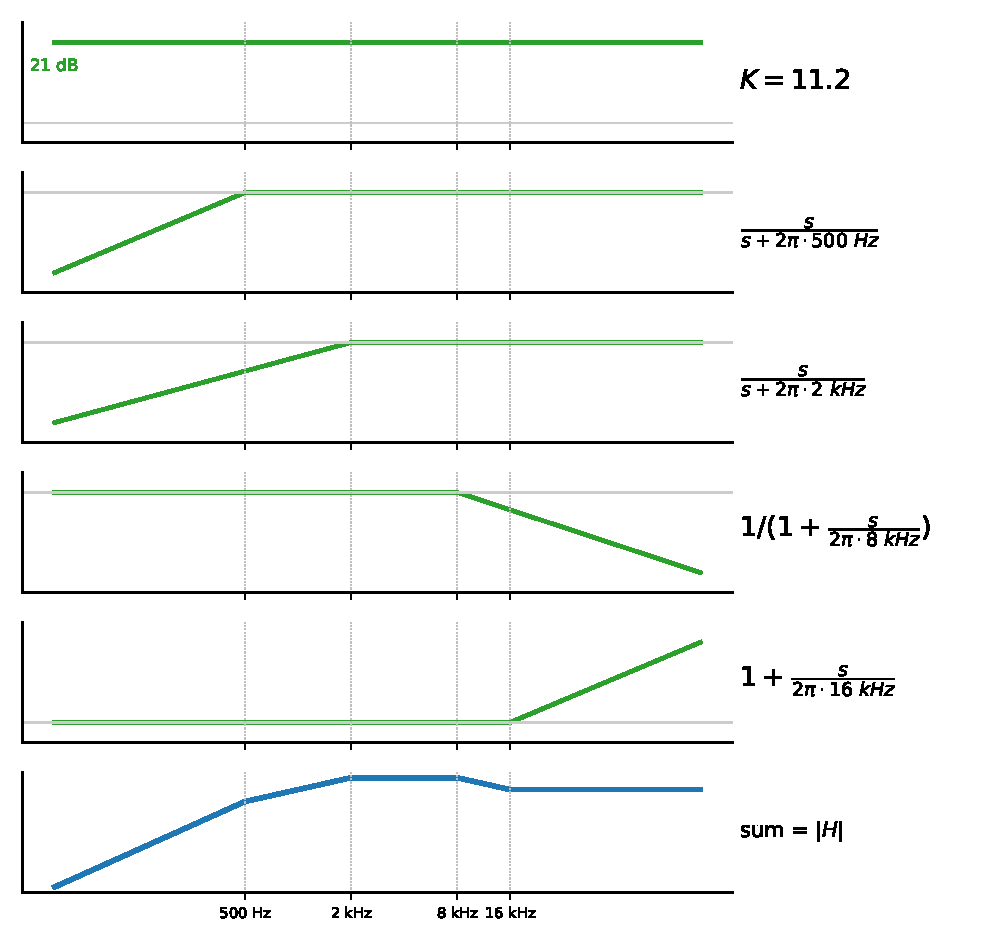
\includegraphics[width=0.82\linewidth,height=9cm,keepaspectratio]{p13_factors}\end{center}
\begin{center}\renewcommand{\arraystretch}{1.35}
\begin{tabular}{lcl}
\toprule
frequency range & slope & asymptote level \\
\midrule
$f<$ 500 Hz & $+40$ dB/dec & 8.98 dB at end \\
500 Hz -- 2 kHz & $+20$ dB/dec & 8.98 dB at start, 21 dB at end \\
2 kHz -- 8 kHz & $0$ dB/dec & 21 dB at start, 21 dB at end \\
8 kHz -- 16 kHz & $-20$ dB/dec & 21 dB at start, 15 dB at end \\
$f>$ 16 kHz & $0$ dB/dec & 15 dB at start \\
\bottomrule
\end{tabular}\end{center}

\solstep{6}{Steady-state output}The input is $V_i(t) = 0.3\sin\left(2\pi\cdot 10000\,t\right)$, so $\omega_{in} = 2\pi\cdot 10000 = 62800$\,rad/s. Put $s=j\omega_{in}$ in each factor (tool T5; use the \emph{exact} factors here, not the straight lines): magnitudes multiply, angles add.
{\small Rules: $\left|\frac{s}{s+p}\right| = \frac{\omega}{\sqrt{\omega^2+p^2}}$, $\angle = \frac{\pi}{2}-\tan^{-1}\frac{\omega}{p}$;\quad $\left|\frac{1}{1+s/p}\right| = \frac{1}{\sqrt{1+(\omega/p)^2}}$, $\angle = -\tan^{-1}\frac{\omega}{p}$;\quad $\left|1+\frac{s}{z}\right| = \sqrt{1+(\omega/z)^2}$, $\angle = \tan^{-1}\frac{\omega}{z}$;\quad a negative $K$ adds $-\pi$.}
\begin{center}\renewcommand{\arraystretch}{1.35}
\begin{tabular}{ccc}
\toprule
factor & magnitude & angle (rad) \\
\midrule
$11.2$ & $11.25$ & $0$ \\
$\rule[-1.1em]{0pt}{2.8em}\dfrac{s}{s+2\pi\cdot 500}$ & $0.9988$ & $0.05$ \\
$\rule[-1.1em]{0pt}{2.8em}\dfrac{s}{s+2\pi\cdot 2\mathrm{k}}$ & $0.9806$ & $0.197$ \\
$\rule[-1.7em]{0pt}{4em}\dfrac{1}{1+\dfrac{s}{2\pi\cdot 8\mathrm{k}}}$ & $0.6247$ & $-0.896$ \\
$\rule[-1.1em]{0pt}{2.8em}\left(1+\dfrac{s}{2\pi\cdot 16\mathrm{k}}\right)$ & $1.179$ & $0.559$ \\
\textbf{total} & $\mathbf{8.114}$ (product) & $\mathbf{-0.0901}$ (sum) \\
\bottomrule
\end{tabular}\end{center}

\begin{align*}
|H(j\omega_{in})| &= 8.11, \qquad \angle H(j\omega_{in}) = -0.0901\ \mathrm{rad} \\
v_{o,ac}(t) &= 8.11\times 0.3\,\sin\left(2\pi\cdot 10000\,t - 0.0901\right) = 2.43\,\sin\left(2\pi\cdot 10000\,t - 0.0901\right)
\end{align*}

\[
\boxed{V_o(t) = 2.43\,\sin\left(2\pi\cdot 10000\,t - 0.0901\right)\ \mathrm{V}}
\]

\begin{ansbox}
$H(s) = 11.2\,\dfrac{s}{s+2\pi\cdot 500}\,\dfrac{s}{s+2\pi\cdot 2\mathrm{k}}\,\dfrac{1}{1+\dfrac{s}{2\pi\cdot 8\mathrm{k}}}\,\left(1+\dfrac{s}{2\pi\cdot 16\mathrm{k}}\right)$\quad (corners: 500 Hz, 2 kHz, 8 kHz, 16 kHz)\\[4pt]
$V_o(t) = 2.43\,\sin\left(2\pi\cdot 10000\,t - 0.0901\right)\ \mathrm{V}$
\end{ansbox}

\newpage
\subsection*{Solution 1D.14 \hfill Hard}
\begin{center}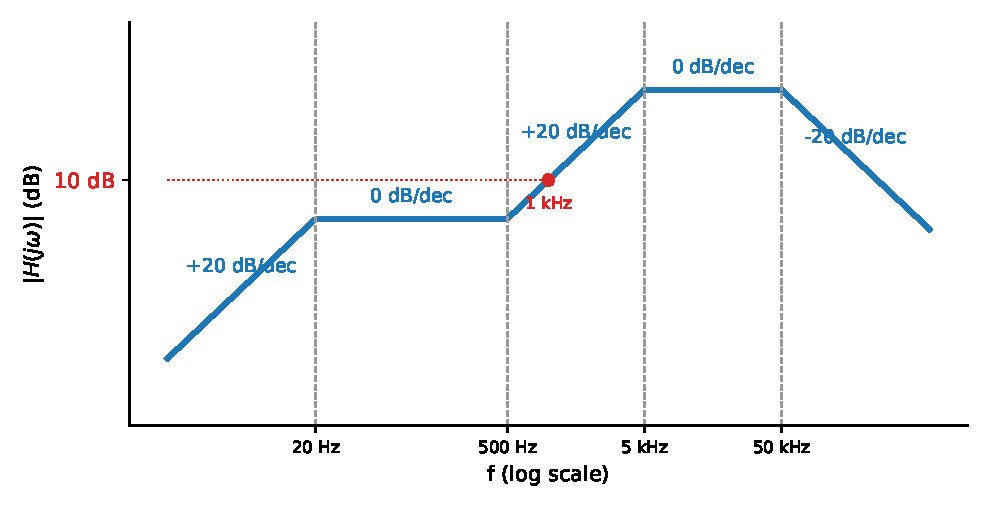
\includegraphics[width=0.7\linewidth,height=5cm,keepaspectratio]{p14_plot}\end{center}
\solstep{1}{Read the corners and slopes}Go left to right along the plot and write down the slope of every straight segment. At each corner frequency the slope changes by a multiple of 20\,dB/dec: every $-20$ is one pole, every $+20$ is one zero (tool T6 read backwards).\begin{center}\renewcommand{\arraystretch}{1.35}
\begin{tabular}{ccccl}
\toprule
corner $f_c$ & slope before & slope after & change & meaning \\
\midrule
20 Hz & $+20$ & $0$ & $-20$ & one pole at $f_c$ \\
500 Hz & $0$ & $+20$ & $+20$ & one zero at $f_c$ \\
5 kHz & $+20$ & $0$ & $-20$ & one pole at $f_c$ \\
50 kHz & $0$ & $-20$ & $-20$ & one pole at $f_c$ \\
\bottomrule
\end{tabular}\end{center}

\solstep{2}{Starting slope $\Rightarrow$ factors of $s$}The plot starts with a slope of $+20$\,dB/dec, i.e. $|H|\propto\omega^1$ at low frequency: the numerator contains $s$. As in class, pair each $s$ with one of the \emph{lowest} poles (20 Hz) as $\frac{s}{s+p}$: such a factor rises at $+20$\,dB/dec below $p$ and is $\approx1$ (0\,dB) above it. The remaining poles are written $\frac{1}{1+s/p}$ and the zeros $\left(1+\frac{s}{z}\right)$. Every corner is an angular frequency $\omega_c=2\pi f_c$.
\solstep{3}{Assemble $H(s)$}Put one factor per pole/zero in front of an unknown constant $K$:\[
H(s) = K\,\dfrac{s}{s+2\pi\cdot 20}\,\left(1+\dfrac{s}{2\pi\cdot 500}\right)\,\dfrac{1}{1+\dfrac{s}{2\pi\cdot 5\mathrm{k}}}\,\dfrac{1}{1+\dfrac{s}{2\pi\cdot 50\mathrm{k}}}
\]

\solstep{4}{Find $K$ from the marked level}The plot marks the level $10$\,dB at $f=$\,1 kHz. On the straight-line plot every factor is either exactly 0\,dB (where it is $\approx1$) or a $\pm20$\,dB/dec line, so evaluate the \emph{asymptote} of each factor at that frequency (the level of a line with slope $\pm20$\,dB/dec is $\pm20\log_{10}(f/f_c)$):\begin{center}\renewcommand{\arraystretch}{1.35}
\begin{tabular}{cccc}
\toprule
factor & $f_c$ & at $f=$\,1 kHz & asymptote (dB) \\
\midrule
$\rule[-1.1em]{0pt}{2.8em}\dfrac{s}{s+2\pi\cdot 20}$ & 20 Hz & $f>f_c$: $\approx 1$ & $0$ \\
$\rule[-1.1em]{0pt}{2.8em}\left(1+\dfrac{s}{2\pi\cdot 500}\right)$ & 500 Hz & $f>f_c$: $\approx \frac{\omega}{z}$ & $6.02$ \\
$\rule[-1.7em]{0pt}{4em}\dfrac{1}{1+\dfrac{s}{2\pi\cdot 5\mathrm{k}}}$ & 5 kHz & $f<f_c$: $\approx 1$ & $0$ \\
$\rule[-1.7em]{0pt}{4em}\dfrac{1}{1+\dfrac{s}{2\pi\cdot 50\mathrm{k}}}$ & 50 kHz & $f<f_c$: $\approx 1$ & $0$ \\
\textbf{sum} &  &  & $\mathbf{6.02}$ \\
\bottomrule
\end{tabular}\end{center}
The dB values of the factors \emph{add} (magnitudes multiply), so\[
20\log_{10}K = 10 - (6.02) = 3.98\ \mathrm{dB}\quad\Rightarrow\quad K = 10^{3.98/20} = 1.58
\]

So\[
\boxed{H(s) = 1.58\,\dfrac{s}{s+2\pi\cdot 20}\,\left(1+\dfrac{s}{2\pi\cdot 500}\right)\,\dfrac{1}{1+\dfrac{s}{2\pi\cdot 5\mathrm{k}}}\,\dfrac{1}{1+\dfrac{s}{2\pi\cdot 50\mathrm{k}}}}
\]

\solstep{5}{Check}Rebuild the plot from the factors: each factor's straight-line plot (green) is added to get $|H|$ (blue). It must reproduce every slope of the given plot and the marked level.\begin{center}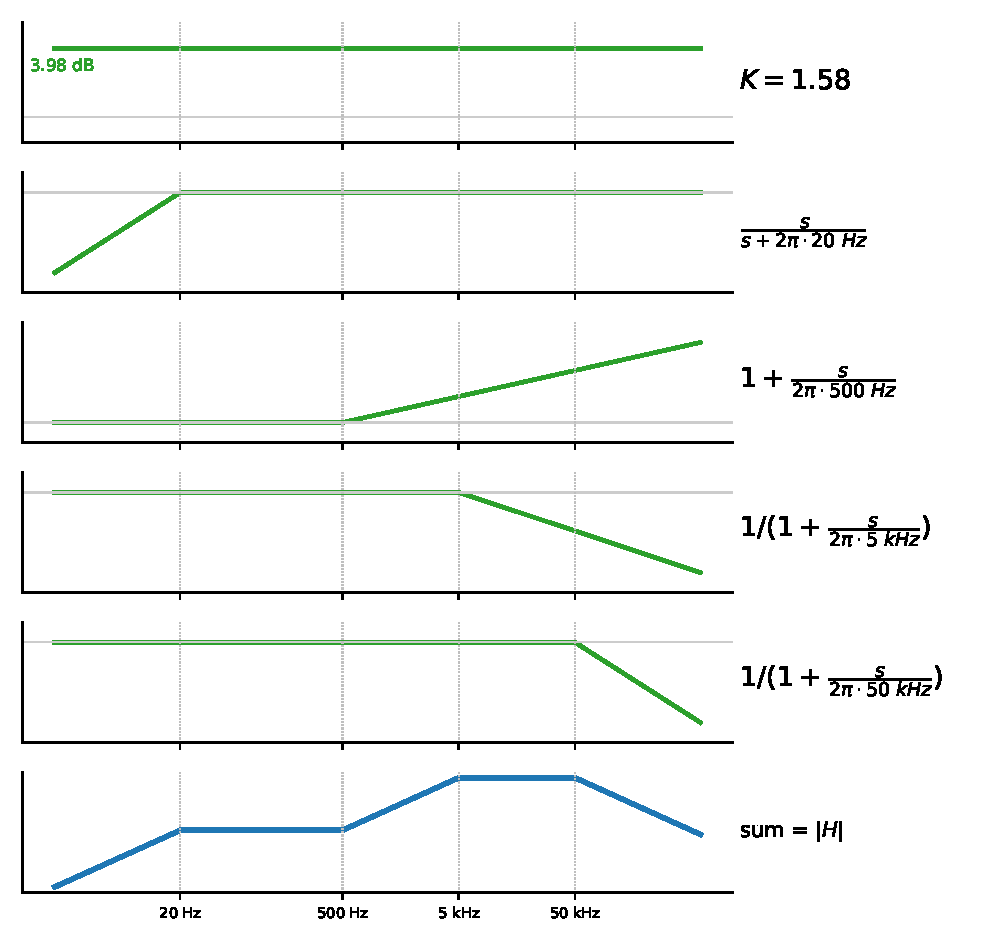
\includegraphics[width=0.82\linewidth,height=9cm,keepaspectratio]{p14_factors}\end{center}
\begin{center}\renewcommand{\arraystretch}{1.35}
\begin{tabular}{lcl}
\toprule
frequency range & slope & asymptote level \\
\midrule
$f<$ 20 Hz & $+20$ dB/dec & 3.98 dB at end \\
20 Hz -- 500 Hz & $0$ dB/dec & 3.98 dB at start, 3.98 dB at end \\
500 Hz -- 5 kHz & $+20$ dB/dec & 3.98 dB at start, 24 dB at end \\
5 kHz -- 50 kHz & $0$ dB/dec & 24 dB at start, 24 dB at end \\
$f>$ 50 kHz & $-20$ dB/dec & 24 dB at start \\
\bottomrule
\end{tabular}\end{center}

\solstep{6}{Steady-state output}The input is $V_i(t) = 0.2\sin\left(2\pi\cdot 2000\,t+\frac{\pi}{3}\right)$, so $\omega_{in} = 2\pi\cdot 2000 = 12600$\,rad/s. Put $s=j\omega_{in}$ in each factor (tool T5; use the \emph{exact} factors here, not the straight lines): magnitudes multiply, angles add.
{\small Rules: $\left|\frac{s}{s+p}\right| = \frac{\omega}{\sqrt{\omega^2+p^2}}$, $\angle = \frac{\pi}{2}-\tan^{-1}\frac{\omega}{p}$;\quad $\left|\frac{1}{1+s/p}\right| = \frac{1}{\sqrt{1+(\omega/p)^2}}$, $\angle = -\tan^{-1}\frac{\omega}{p}$;\quad $\left|1+\frac{s}{z}\right| = \sqrt{1+(\omega/z)^2}$, $\angle = \tan^{-1}\frac{\omega}{z}$;\quad a negative $K$ adds $-\pi$.}
\begin{center}\renewcommand{\arraystretch}{1.35}
\begin{tabular}{ccc}
\toprule
factor & magnitude & angle (rad) \\
\midrule
$1.58$ & $1.581$ & $0$ \\
$\rule[-1.1em]{0pt}{2.8em}\dfrac{s}{s+2\pi\cdot 20}$ & $1$ & $0.01$ \\
$\rule[-1.1em]{0pt}{2.8em}\left(1+\dfrac{s}{2\pi\cdot 500}\right)$ & $4.123$ & $1.33$ \\
$\rule[-1.7em]{0pt}{4em}\dfrac{1}{1+\dfrac{s}{2\pi\cdot 5\mathrm{k}}}$ & $0.9285$ & $-0.381$ \\
$\rule[-1.7em]{0pt}{4em}\dfrac{1}{1+\dfrac{s}{2\pi\cdot 50\mathrm{k}}}$ & $0.9992$ & $-0.04$ \\
\textbf{total} & $\mathbf{6.048}$ (product) & $\mathbf{0.915}$ (sum) \\
\bottomrule
\end{tabular}\end{center}

\begin{align*}
|H(j\omega_{in})| &= 6.05, \qquad \angle H(j\omega_{in}) = 0.915\ \mathrm{rad} \\
v_{o,ac}(t) &= 6.05\times 0.2\,\sin\left(2\pi\cdot 2000\,t + 1.96\right) = 1.21\,\sin\left(2\pi\cdot 2000\,t + 1.96\right)
\end{align*}

(phase: $\theta + \angle H = \frac{\pi}{3} + (0.915) = 1.96$\,rad.)
\[
\boxed{V_o(t) = 1.21\,\sin\left(2\pi\cdot 2000\,t + 1.96\right)\ \mathrm{V}}
\]

\begin{ansbox}
$H(s) = 1.58\,\dfrac{s}{s+2\pi\cdot 20}\,\left(1+\dfrac{s}{2\pi\cdot 500}\right)\,\dfrac{1}{1+\dfrac{s}{2\pi\cdot 5\mathrm{k}}}\,\dfrac{1}{1+\dfrac{s}{2\pi\cdot 50\mathrm{k}}}$\quad (corners: 20 Hz, 500 Hz, 5 kHz, 50 kHz)\\[4pt]
$V_o(t) = 1.21\,\sin\left(2\pi\cdot 2000\,t + 1.96\right)\ \mathrm{V}$
\end{ansbox}

\newpage
\subsection*{Solution 1D.15 \hfill Hard}
\begin{center}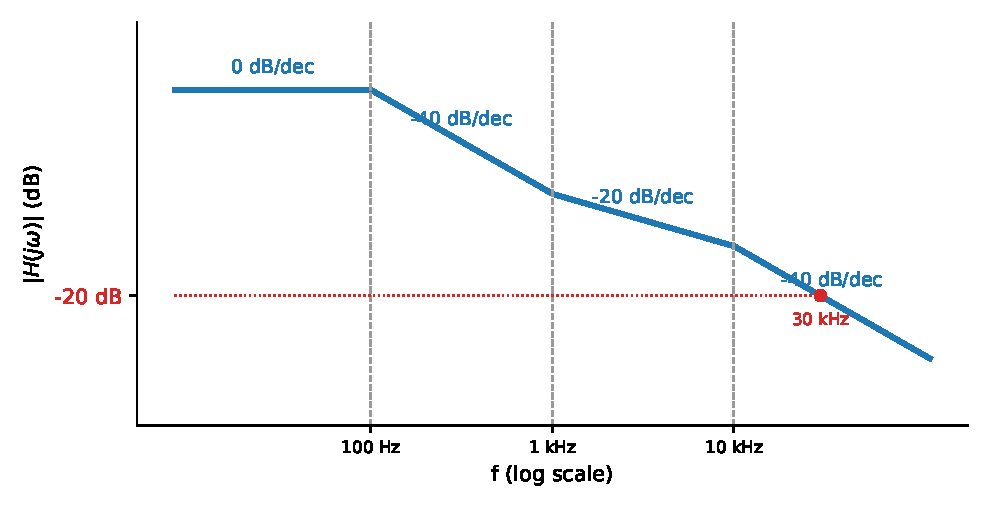
\includegraphics[width=0.7\linewidth,height=5cm,keepaspectratio]{p15_plot}\end{center}
\solstep{1}{Read the corners and slopes}Go left to right along the plot and write down the slope of every straight segment. At each corner frequency the slope changes by a multiple of 20\,dB/dec: every $-20$ is one pole, every $+20$ is one zero (tool T6 read backwards).\begin{center}\renewcommand{\arraystretch}{1.35}
\begin{tabular}{ccccl}
\toprule
corner $f_c$ & slope before & slope after & change & meaning \\
\midrule
100 Hz & $0$ & $-40$ & $-40$ & two poles at $f_c$ \\
1 kHz & $-40$ & $-20$ & $+20$ & one zero at $f_c$ \\
10 kHz & $-20$ & $-40$ & $-20$ & one pole at $f_c$ \\
\bottomrule
\end{tabular}\end{center}

\solstep{2}{Starting slope $\Rightarrow$ factors of $s$}The plot starts \emph{flat} (0\,dB/dec), so there is no factor $s$ in the numerator: every pole is written as $\frac{1}{1+s/p}$ and every zero as $\left(1+\frac{s}{z}\right)$, which are all $\approx1$ (0\,dB) at low frequency. Every corner is an angular frequency $\omega_c=2\pi f_c$.
\solstep{3}{Assemble $H(s)$}Put one factor per pole/zero in front of an unknown constant $K$:\[
H(s) = K\,\dfrac{1}{1+\dfrac{s}{2\pi\cdot 100}}\,\dfrac{1}{1+\dfrac{s}{2\pi\cdot 100}}\,\left(1+\dfrac{s}{2\pi\cdot 1\mathrm{k}}\right)\,\dfrac{1}{1+\dfrac{s}{2\pi\cdot 10\mathrm{k}}}
\]

\solstep{4}{Find $K$ from the marked level}The plot marks the level $-20$\,dB at $f=$\,30 kHz. On the straight-line plot every factor is either exactly 0\,dB (where it is $\approx1$) or a $\pm20$\,dB/dec line, so evaluate the \emph{asymptote} of each factor at that frequency (the level of a line with slope $\pm20$\,dB/dec is $\pm20\log_{10}(f/f_c)$):\begin{center}\renewcommand{\arraystretch}{1.35}
\begin{tabular}{cccc}
\toprule
factor & $f_c$ & at $f=$\,30 kHz & asymptote (dB) \\
\midrule
$\rule[-1.7em]{0pt}{4em}\dfrac{1}{1+\dfrac{s}{2\pi\cdot 100}}$ & 100 Hz & $f>f_c$: $\approx \frac{p}{\omega}$ & $-49.5$ \\
$\rule[-1.7em]{0pt}{4em}\dfrac{1}{1+\dfrac{s}{2\pi\cdot 100}}$ & 100 Hz & $f>f_c$: $\approx \frac{p}{\omega}$ & $-49.5$ \\
$\rule[-1.1em]{0pt}{2.8em}\left(1+\dfrac{s}{2\pi\cdot 1\mathrm{k}}\right)$ & 1 kHz & $f>f_c$: $\approx \frac{\omega}{z}$ & $29.5$ \\
$\rule[-1.7em]{0pt}{4em}\dfrac{1}{1+\dfrac{s}{2\pi\cdot 10\mathrm{k}}}$ & 10 kHz & $f>f_c$: $\approx \frac{p}{\omega}$ & $-9.54$ \\
\textbf{sum} &  &  & $\mathbf{-79.1}$ \\
\bottomrule
\end{tabular}\end{center}
The dB values of the factors \emph{add} (magnitudes multiply), so\[
20\log_{10}K = -20 - (-79.1) = 59.1\ \mathrm{dB}\quad\Rightarrow\quad K = 10^{59.1/20} = 900
\]

So\[
\boxed{H(s) = 900\,\dfrac{1}{1+\dfrac{s}{2\pi\cdot 100}}\,\dfrac{1}{1+\dfrac{s}{2\pi\cdot 100}}\,\left(1+\dfrac{s}{2\pi\cdot 1\mathrm{k}}\right)\,\dfrac{1}{1+\dfrac{s}{2\pi\cdot 10\mathrm{k}}}}
\]

\solstep{5}{Check}Rebuild the plot from the factors: each factor's straight-line plot (green) is added to get $|H|$ (blue). It must reproduce every slope of the given plot and the marked level.\begin{center}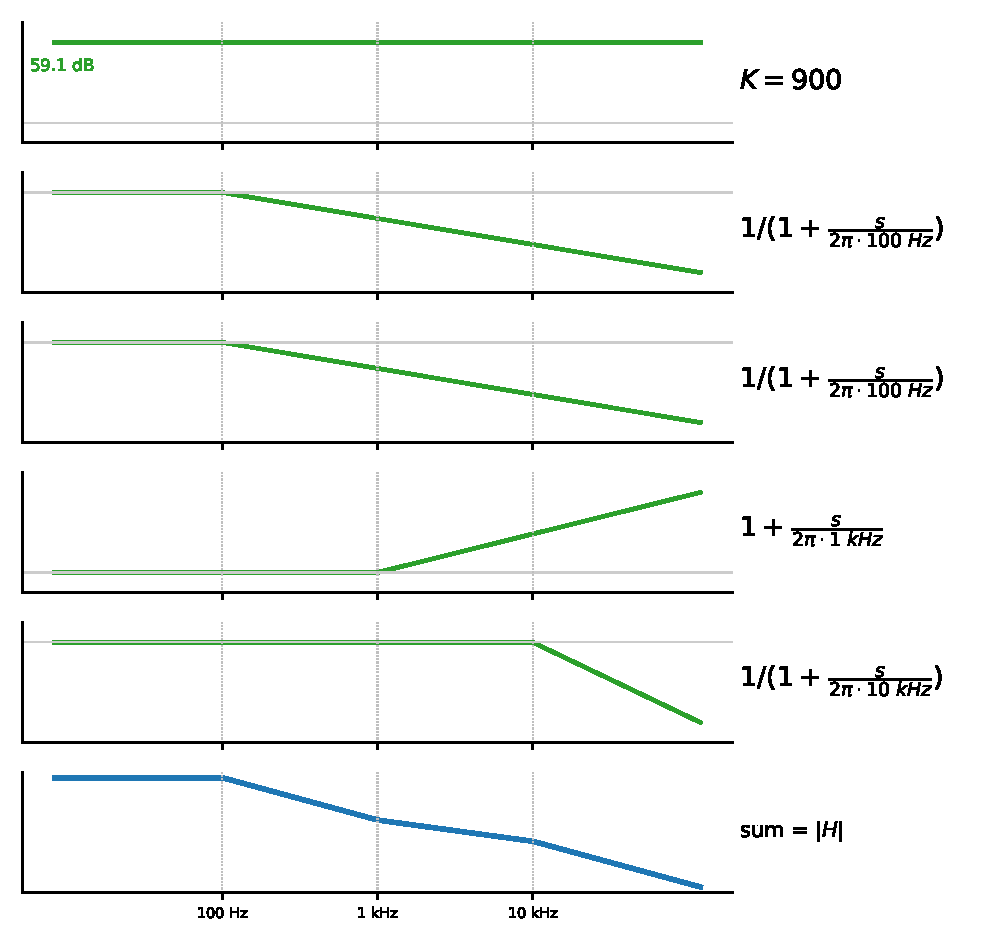
\includegraphics[width=0.82\linewidth,height=9cm,keepaspectratio]{p15_factors}\end{center}
\begin{center}\renewcommand{\arraystretch}{1.35}
\begin{tabular}{lcl}
\toprule
frequency range & slope & asymptote level \\
\midrule
$f<$ 100 Hz & $0$ dB/dec & 59.1 dB at end \\
100 Hz -- 1 kHz & $-40$ dB/dec & 59.1 dB at start, 19.1 dB at end \\
1 kHz -- 10 kHz & $-20$ dB/dec & 19.1 dB at start, -0.915 dB at end \\
$f>$ 10 kHz & $-40$ dB/dec & -0.915 dB at start \\
\bottomrule
\end{tabular}\end{center}

\solstep{6}{Steady-state output}The input is $V_i(t) = 0.1\sin\left(2\pi\cdot 300\,t\right)$, so $\omega_{in} = 2\pi\cdot 300 = 1880$\,rad/s. Put $s=j\omega_{in}$ in each factor (tool T5; use the \emph{exact} factors here, not the straight lines): magnitudes multiply, angles add.
{\small Rules: $\left|\frac{s}{s+p}\right| = \frac{\omega}{\sqrt{\omega^2+p^2}}$, $\angle = \frac{\pi}{2}-\tan^{-1}\frac{\omega}{p}$;\quad $\left|\frac{1}{1+s/p}\right| = \frac{1}{\sqrt{1+(\omega/p)^2}}$, $\angle = -\tan^{-1}\frac{\omega}{p}$;\quad $\left|1+\frac{s}{z}\right| = \sqrt{1+(\omega/z)^2}$, $\angle = \tan^{-1}\frac{\omega}{z}$;\quad a negative $K$ adds $-\pi$.}
\begin{center}\renewcommand{\arraystretch}{1.35}
\begin{tabular}{ccc}
\toprule
factor & magnitude & angle (rad) \\
\midrule
$900$ & $900$ & $0$ \\
$\rule[-1.7em]{0pt}{4em}\dfrac{1}{1+\dfrac{s}{2\pi\cdot 100}}$ & $0.3162$ & $-1.25$ \\
$\rule[-1.7em]{0pt}{4em}\dfrac{1}{1+\dfrac{s}{2\pi\cdot 100}}$ & $0.3162$ & $-1.25$ \\
$\rule[-1.1em]{0pt}{2.8em}\left(1+\dfrac{s}{2\pi\cdot 1\mathrm{k}}\right)$ & $1.044$ & $0.291$ \\
$\rule[-1.7em]{0pt}{4em}\dfrac{1}{1+\dfrac{s}{2\pi\cdot 10\mathrm{k}}}$ & $0.9996$ & $-0.03$ \\
\textbf{total} & $\mathbf{93.92}$ (product) & $\mathbf{-2.24}$ (sum) \\
\bottomrule
\end{tabular}\end{center}

\begin{align*}
|H(j\omega_{in})| &= 93.9, \qquad \angle H(j\omega_{in}) = -2.24\ \mathrm{rad} \\
v_{o,ac}(t) &= 93.9\times 0.1\,\sin\left(2\pi\cdot 300\,t - 2.24\right) = 9.39\,\sin\left(2\pi\cdot 300\,t - 2.24\right)
\end{align*}

\[
\boxed{V_o(t) = 9.39\,\sin\left(2\pi\cdot 300\,t - 2.24\right)\ \mathrm{V}}
\]

\begin{ansbox}
$H(s) = 900\,\dfrac{1}{1+\dfrac{s}{2\pi\cdot 100}}\,\dfrac{1}{1+\dfrac{s}{2\pi\cdot 100}}\,\left(1+\dfrac{s}{2\pi\cdot 1\mathrm{k}}\right)\,\dfrac{1}{1+\dfrac{s}{2\pi\cdot 10\mathrm{k}}}$\quad (corners: 100 Hz, 100 Hz, 1 kHz, 10 kHz)\\[4pt]
$V_o(t) = 9.39\,\sin\left(2\pi\cdot 300\,t - 2.24\right)\ \mathrm{V}$
\end{ansbox}

\newpage
\subsection*{Solution 1D.16 \hfill Hard}
\begin{center}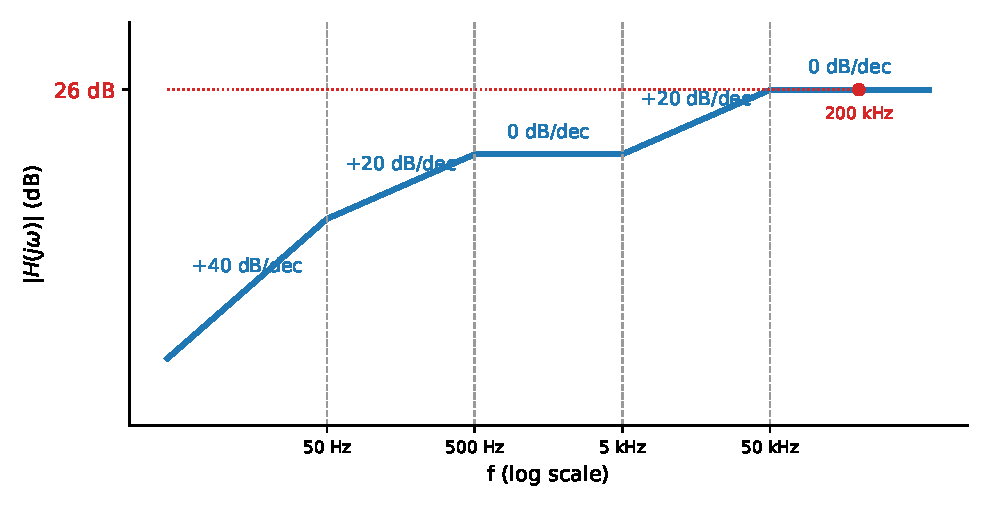
\includegraphics[width=0.7\linewidth,height=5cm,keepaspectratio]{p16_plot}\end{center}
\solstep{1}{Read the corners and slopes}Go left to right along the plot and write down the slope of every straight segment. At each corner frequency the slope changes by a multiple of 20\,dB/dec: every $-20$ is one pole, every $+20$ is one zero (tool T6 read backwards).\begin{center}\renewcommand{\arraystretch}{1.35}
\begin{tabular}{ccccl}
\toprule
corner $f_c$ & slope before & slope after & change & meaning \\
\midrule
50 Hz & $+40$ & $+20$ & $-20$ & one pole at $f_c$ \\
500 Hz & $+20$ & $0$ & $-20$ & one pole at $f_c$ \\
5 kHz & $0$ & $+20$ & $+20$ & one zero at $f_c$ \\
50 kHz & $+20$ & $0$ & $-20$ & one pole at $f_c$ \\
\bottomrule
\end{tabular}\end{center}

\solstep{2}{Starting slope $\Rightarrow$ factors of $s$}The plot starts with a slope of $+40$\,dB/dec, i.e. $|H|\propto\omega^2$ at low frequency: the numerator contains $s^2$. As in class, pair each $s$ with one of the \emph{lowest} poles (50 Hz, 500 Hz) as $\frac{s}{s+p}$: such a factor rises at $+20$\,dB/dec below $p$ and is $\approx1$ (0\,dB) above it. The remaining poles are written $\frac{1}{1+s/p}$ and the zeros $\left(1+\frac{s}{z}\right)$. Every corner is an angular frequency $\omega_c=2\pi f_c$.
\solstep{3}{Assemble $H(s)$}Put one factor per pole/zero in front of an unknown constant $K$:\[
H(s) = K\,\dfrac{s}{s+2\pi\cdot 50}\,\dfrac{s}{s+2\pi\cdot 500}\,\left(1+\dfrac{s}{2\pi\cdot 5\mathrm{k}}\right)\,\dfrac{1}{1+\dfrac{s}{2\pi\cdot 50\mathrm{k}}}
\]

\solstep{4}{Find $K$ from the marked level}The plot marks the level $26$\,dB at $f=$\,200 kHz. On the straight-line plot every factor is either exactly 0\,dB (where it is $\approx1$) or a $\pm20$\,dB/dec line, so evaluate the \emph{asymptote} of each factor at that frequency (the level of a line with slope $\pm20$\,dB/dec is $\pm20\log_{10}(f/f_c)$):\begin{center}\renewcommand{\arraystretch}{1.35}
\begin{tabular}{cccc}
\toprule
factor & $f_c$ & at $f=$\,200 kHz & asymptote (dB) \\
\midrule
$\rule[-1.1em]{0pt}{2.8em}\dfrac{s}{s+2\pi\cdot 50}$ & 50 Hz & $f>f_c$: $\approx 1$ & $0$ \\
$\rule[-1.1em]{0pt}{2.8em}\dfrac{s}{s+2\pi\cdot 500}$ & 500 Hz & $f>f_c$: $\approx 1$ & $0$ \\
$\rule[-1.1em]{0pt}{2.8em}\left(1+\dfrac{s}{2\pi\cdot 5\mathrm{k}}\right)$ & 5 kHz & $f>f_c$: $\approx \frac{\omega}{z}$ & $32$ \\
$\rule[-1.7em]{0pt}{4em}\dfrac{1}{1+\dfrac{s}{2\pi\cdot 50\mathrm{k}}}$ & 50 kHz & $f>f_c$: $\approx \frac{p}{\omega}$ & $-12$ \\
\textbf{sum} &  &  & $\mathbf{20}$ \\
\bottomrule
\end{tabular}\end{center}
The dB values of the factors \emph{add} (magnitudes multiply), so\[
20\log_{10}K = 26 - (20) = 6\ \mathrm{dB}\quad\Rightarrow\quad K = 10^{6/20} = 2
\]

So\[
\boxed{H(s) = 2\,\dfrac{s}{s+2\pi\cdot 50}\,\dfrac{s}{s+2\pi\cdot 500}\,\left(1+\dfrac{s}{2\pi\cdot 5\mathrm{k}}\right)\,\dfrac{1}{1+\dfrac{s}{2\pi\cdot 50\mathrm{k}}}}
\]

\solstep{5}{Check}Rebuild the plot from the factors: each factor's straight-line plot (green) is added to get $|H|$ (blue). It must reproduce every slope of the given plot and the marked level.\begin{center}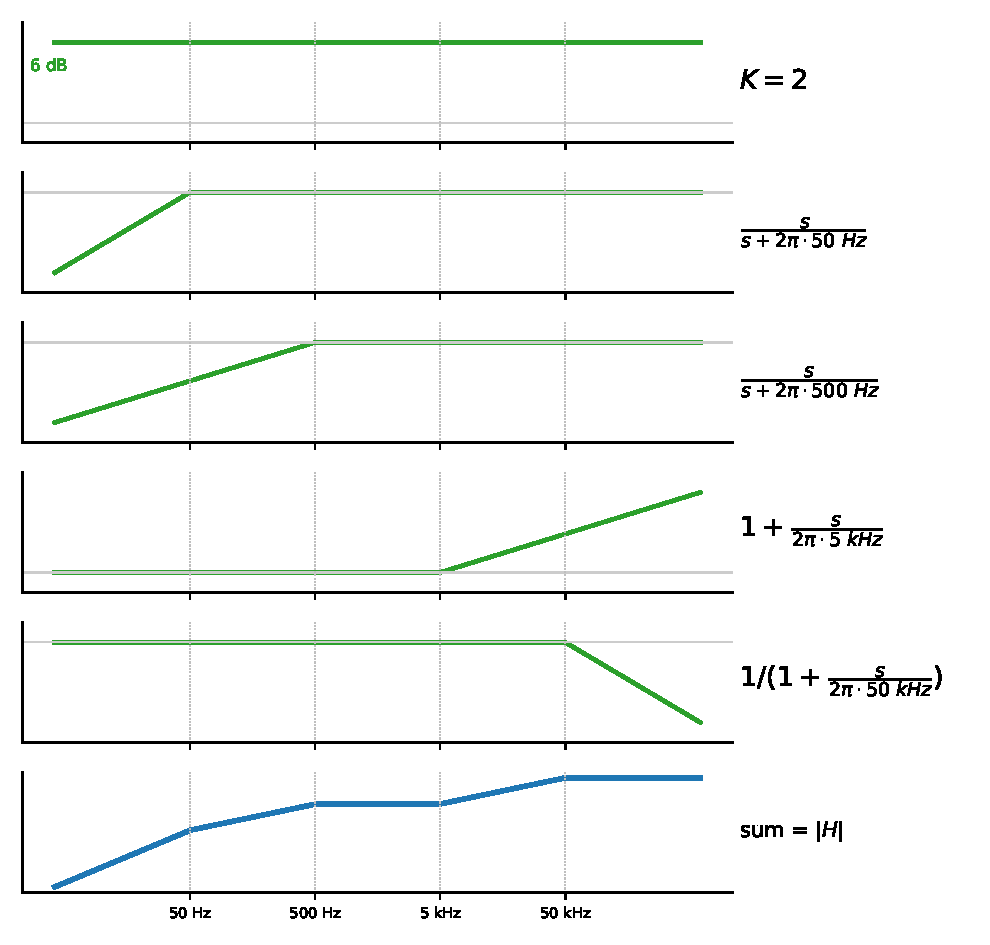
\includegraphics[width=0.82\linewidth,height=9cm,keepaspectratio]{p16_factors}\end{center}
\begin{center}\renewcommand{\arraystretch}{1.35}
\begin{tabular}{lcl}
\toprule
frequency range & slope & asymptote level \\
\midrule
$f<$ 50 Hz & $+40$ dB/dec & -14 dB at end \\
50 Hz -- 500 Hz & $+20$ dB/dec & -14 dB at start, 6 dB at end \\
500 Hz -- 5 kHz & $0$ dB/dec & 6 dB at start, 6 dB at end \\
5 kHz -- 50 kHz & $+20$ dB/dec & 6 dB at start, 26 dB at end \\
$f>$ 50 kHz & $0$ dB/dec & 26 dB at start \\
\bottomrule
\end{tabular}\end{center}

\solstep{6}{Steady-state output}The input is $V_i(t) = 0.05\cos\left(2\pi\cdot 1000\,t-\frac{\pi}{6}\right)$, so $\omega_{in} = 2\pi\cdot 1000 = 6280$\,rad/s. Put $s=j\omega_{in}$ in each factor (tool T5; use the \emph{exact} factors here, not the straight lines): magnitudes multiply, angles add.
{\small Rules: $\left|\frac{s}{s+p}\right| = \frac{\omega}{\sqrt{\omega^2+p^2}}$, $\angle = \frac{\pi}{2}-\tan^{-1}\frac{\omega}{p}$;\quad $\left|\frac{1}{1+s/p}\right| = \frac{1}{\sqrt{1+(\omega/p)^2}}$, $\angle = -\tan^{-1}\frac{\omega}{p}$;\quad $\left|1+\frac{s}{z}\right| = \sqrt{1+(\omega/z)^2}$, $\angle = \tan^{-1}\frac{\omega}{z}$;\quad a negative $K$ adds $-\pi$.}
\begin{center}\renewcommand{\arraystretch}{1.35}
\begin{tabular}{ccc}
\toprule
factor & magnitude & angle (rad) \\
\midrule
$2$ & $1.995$ & $0$ \\
$\rule[-1.1em]{0pt}{2.8em}\dfrac{s}{s+2\pi\cdot 50}$ & $0.9988$ & $0.05$ \\
$\rule[-1.1em]{0pt}{2.8em}\dfrac{s}{s+2\pi\cdot 500}$ & $0.8944$ & $0.464$ \\
$\rule[-1.1em]{0pt}{2.8em}\left(1+\dfrac{s}{2\pi\cdot 5\mathrm{k}}\right)$ & $1.02$ & $0.197$ \\
$\rule[-1.7em]{0pt}{4em}\dfrac{1}{1+\dfrac{s}{2\pi\cdot 50\mathrm{k}}}$ & $0.9998$ & $-0.02$ \\
\textbf{total} & $\mathbf{1.817}$ (product) & $\mathbf{0.691}$ (sum) \\
\bottomrule
\end{tabular}\end{center}

\begin{align*}
|H(j\omega_{in})| &= 1.82, \qquad \angle H(j\omega_{in}) = 0.691\ \mathrm{rad} \\
v_{o,ac}(t) &= 1.82\times 0.05\,\cos\left(2\pi\cdot 1000\,t + 0.167\right) = 0.0909\,\cos\left(2\pi\cdot 1000\,t + 0.167\right)
\end{align*}

(phase: $\theta + \angle H = -\frac{\pi}{6} + (0.691) = 0.167$\,rad.)
\[
\boxed{V_o(t) = 0.0909\,\cos\left(2\pi\cdot 1000\,t + 0.167\right)\ \mathrm{V}}
\]

\begin{ansbox}
$H(s) = 2\,\dfrac{s}{s+2\pi\cdot 50}\,\dfrac{s}{s+2\pi\cdot 500}\,\left(1+\dfrac{s}{2\pi\cdot 5\mathrm{k}}\right)\,\dfrac{1}{1+\dfrac{s}{2\pi\cdot 50\mathrm{k}}}$\quad (corners: 50 Hz, 500 Hz, 5 kHz, 50 kHz)\\[4pt]
$V_o(t) = 0.0909\,\cos\left(2\pi\cdot 1000\,t + 0.167\right)\ \mathrm{V}$
\end{ansbox}

\newpage
\subsection*{Solution 1D.17 \hfill Hard}
\begin{center}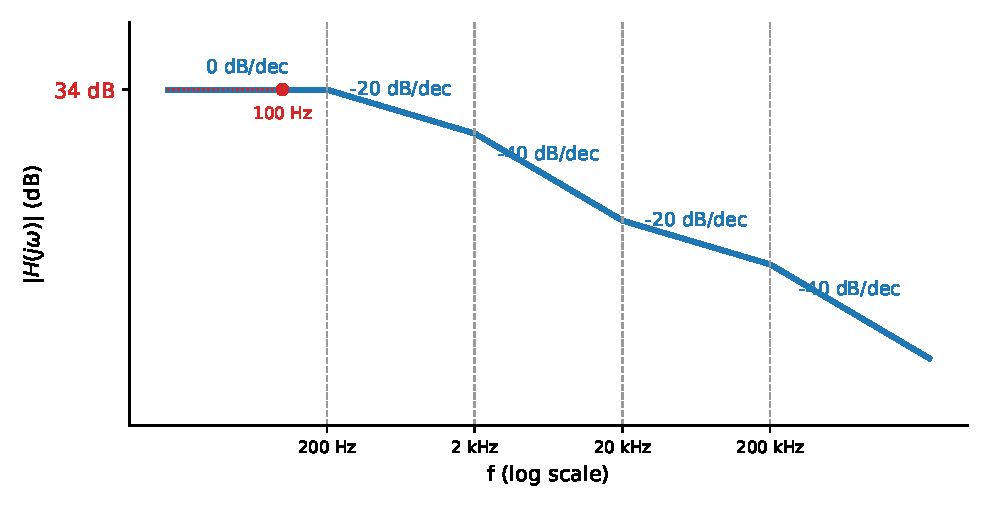
\includegraphics[width=0.7\linewidth,height=5cm,keepaspectratio]{p17_plot}\end{center}
\solstep{1}{Read the corners and slopes}Go left to right along the plot and write down the slope of every straight segment. At each corner frequency the slope changes by a multiple of 20\,dB/dec: every $-20$ is one pole, every $+20$ is one zero (tool T6 read backwards).\begin{center}\renewcommand{\arraystretch}{1.35}
\begin{tabular}{ccccl}
\toprule
corner $f_c$ & slope before & slope after & change & meaning \\
\midrule
200 Hz & $0$ & $-20$ & $-20$ & one pole at $f_c$ \\
2 kHz & $-20$ & $-40$ & $-20$ & one pole at $f_c$ \\
20 kHz & $-40$ & $-20$ & $+20$ & one zero at $f_c$ \\
200 kHz & $-20$ & $-40$ & $-20$ & one pole at $f_c$ \\
\bottomrule
\end{tabular}\end{center}

\solstep{2}{Starting slope $\Rightarrow$ factors of $s$}The plot starts \emph{flat} (0\,dB/dec), so there is no factor $s$ in the numerator: every pole is written as $\frac{1}{1+s/p}$ and every zero as $\left(1+\frac{s}{z}\right)$, which are all $\approx1$ (0\,dB) at low frequency. Every corner is an angular frequency $\omega_c=2\pi f_c$.
\solstep{3}{Assemble $H(s)$}Put one factor per pole/zero in front of an unknown constant $K$:\[
H(s) = K\,\dfrac{1}{1+\dfrac{s}{2\pi\cdot 200}}\,\dfrac{1}{1+\dfrac{s}{2\pi\cdot 2\mathrm{k}}}\,\left(1+\dfrac{s}{2\pi\cdot 20\mathrm{k}}\right)\,\dfrac{1}{1+\dfrac{s}{2\pi\cdot 200\mathrm{k}}}
\]

\solstep{4}{Find $K$ from the marked level}The plot marks the level $34$\,dB at $f=$\,100 Hz. On the straight-line plot every factor is either exactly 0\,dB (where it is $\approx1$) or a $\pm20$\,dB/dec line, so evaluate the \emph{asymptote} of each factor at that frequency (the level of a line with slope $\pm20$\,dB/dec is $\pm20\log_{10}(f/f_c)$):\begin{center}\renewcommand{\arraystretch}{1.35}
\begin{tabular}{cccc}
\toprule
factor & $f_c$ & at $f=$\,100 Hz & asymptote (dB) \\
\midrule
$\rule[-1.7em]{0pt}{4em}\dfrac{1}{1+\dfrac{s}{2\pi\cdot 200}}$ & 200 Hz & $f<f_c$: $\approx 1$ & $0$ \\
$\rule[-1.7em]{0pt}{4em}\dfrac{1}{1+\dfrac{s}{2\pi\cdot 2\mathrm{k}}}$ & 2 kHz & $f<f_c$: $\approx 1$ & $0$ \\
$\rule[-1.1em]{0pt}{2.8em}\left(1+\dfrac{s}{2\pi\cdot 20\mathrm{k}}\right)$ & 20 kHz & $f<f_c$: $\approx 1$ & $0$ \\
$\rule[-1.7em]{0pt}{4em}\dfrac{1}{1+\dfrac{s}{2\pi\cdot 200\mathrm{k}}}$ & 200 kHz & $f<f_c$: $\approx 1$ & $0$ \\
\textbf{sum} &  &  & $\mathbf{0}$ \\
\bottomrule
\end{tabular}\end{center}
The dB values of the factors \emph{add} (magnitudes multiply), so\[
20\log_{10}K = 34 - (0) = 34\ \mathrm{dB}\quad\Rightarrow\quad K = 10^{34/20} = 50.1
\]

So\[
\boxed{H(s) = 50.1\,\dfrac{1}{1+\dfrac{s}{2\pi\cdot 200}}\,\dfrac{1}{1+\dfrac{s}{2\pi\cdot 2\mathrm{k}}}\,\left(1+\dfrac{s}{2\pi\cdot 20\mathrm{k}}\right)\,\dfrac{1}{1+\dfrac{s}{2\pi\cdot 200\mathrm{k}}}}
\]

\solstep{5}{Check}Rebuild the plot from the factors: each factor's straight-line plot (green) is added to get $|H|$ (blue). It must reproduce every slope of the given plot and the marked level.\begin{center}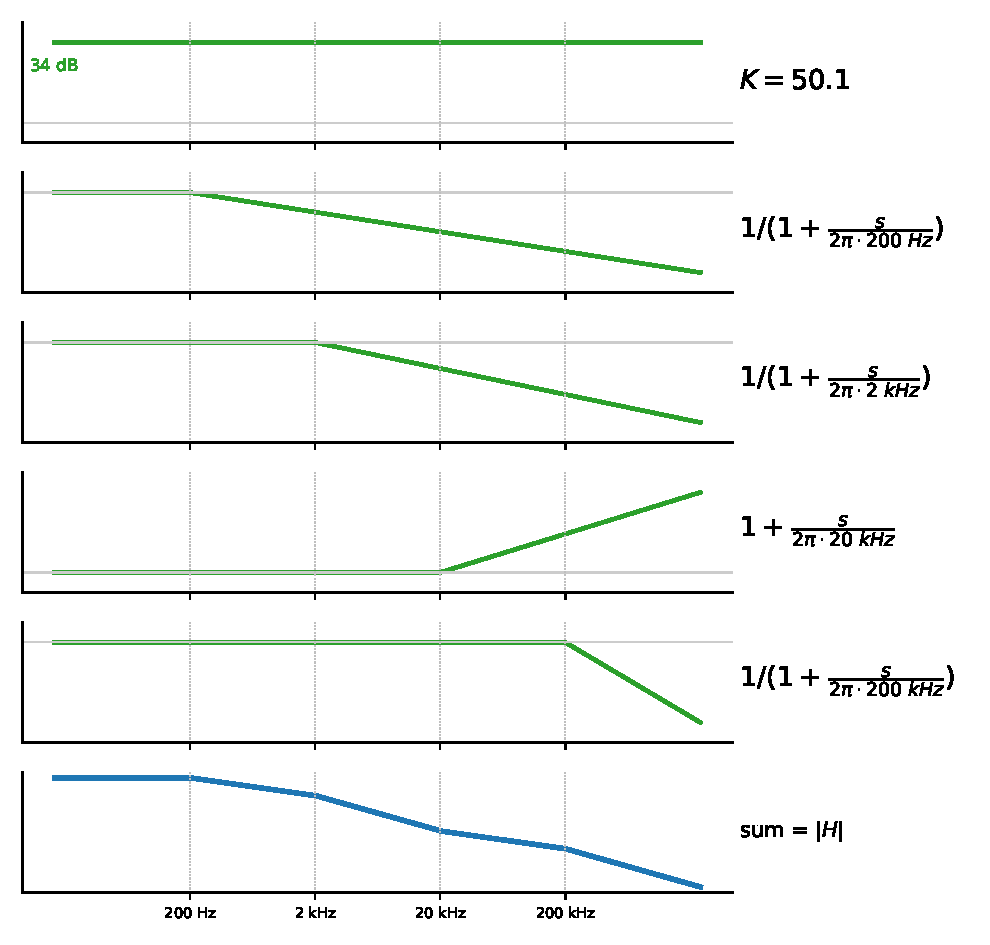
\includegraphics[width=0.82\linewidth,height=9cm,keepaspectratio]{p17_factors}\end{center}
\begin{center}\renewcommand{\arraystretch}{1.35}
\begin{tabular}{lcl}
\toprule
frequency range & slope & asymptote level \\
\midrule
$f<$ 200 Hz & $0$ dB/dec & 34 dB at end \\
200 Hz -- 2 kHz & $-20$ dB/dec & 34 dB at start, 14 dB at end \\
2 kHz -- 20 kHz & $-40$ dB/dec & 14 dB at start, -26 dB at end \\
20 kHz -- 200 kHz & $-20$ dB/dec & -26 dB at start, -46 dB at end \\
$f>$ 200 kHz & $-40$ dB/dec & -46 dB at start \\
\bottomrule
\end{tabular}\end{center}

\solstep{6}{Steady-state output}The input is $V_i(t) = 0.02\sin\left(2\pi\cdot 5000\,t+\frac{\pi}{2}\right)$, so $\omega_{in} = 2\pi\cdot 5000 = 31400$\,rad/s. Put $s=j\omega_{in}$ in each factor (tool T5; use the \emph{exact} factors here, not the straight lines): magnitudes multiply, angles add.
{\small Rules: $\left|\frac{s}{s+p}\right| = \frac{\omega}{\sqrt{\omega^2+p^2}}$, $\angle = \frac{\pi}{2}-\tan^{-1}\frac{\omega}{p}$;\quad $\left|\frac{1}{1+s/p}\right| = \frac{1}{\sqrt{1+(\omega/p)^2}}$, $\angle = -\tan^{-1}\frac{\omega}{p}$;\quad $\left|1+\frac{s}{z}\right| = \sqrt{1+(\omega/z)^2}$, $\angle = \tan^{-1}\frac{\omega}{z}$;\quad a negative $K$ adds $-\pi$.}
\begin{center}\renewcommand{\arraystretch}{1.35}
\begin{tabular}{ccc}
\toprule
factor & magnitude & angle (rad) \\
\midrule
$50.1$ & $50.12$ & $0$ \\
$\rule[-1.7em]{0pt}{4em}\dfrac{1}{1+\dfrac{s}{2\pi\cdot 200}}$ & $0.03997$ & $-1.53$ \\
$\rule[-1.7em]{0pt}{4em}\dfrac{1}{1+\dfrac{s}{2\pi\cdot 2\mathrm{k}}}$ & $0.3714$ & $-1.19$ \\
$\rule[-1.1em]{0pt}{2.8em}\left(1+\dfrac{s}{2\pi\cdot 20\mathrm{k}}\right)$ & $1.031$ & $0.245$ \\
$\rule[-1.7em]{0pt}{4em}\dfrac{1}{1+\dfrac{s}{2\pi\cdot 200\mathrm{k}}}$ & $0.9997$ & $-0.025$ \\
\textbf{total} & $\mathbf{0.7666}$ (product) & $\mathbf{-2.5}$ (sum) \\
\bottomrule
\end{tabular}\end{center}

\begin{align*}
|H(j\omega_{in})| &= 0.767, \qquad \angle H(j\omega_{in}) = -2.5\ \mathrm{rad} \\
v_{o,ac}(t) &= 0.767\times 0.02\,\sin\left(2\pi\cdot 5000\,t - 0.93\right) = 0.0153\,\sin\left(2\pi\cdot 5000\,t - 0.93\right)
\end{align*}

(phase: $\theta + \angle H = \frac{\pi}{2} + (-2.5) = -0.93$\,rad.)
\[
\boxed{V_o(t) = 0.0153\,\sin\left(2\pi\cdot 5000\,t - 0.93\right)\ \mathrm{V}}
\]

\begin{ansbox}
$H(s) = 50.1\,\dfrac{1}{1+\dfrac{s}{2\pi\cdot 200}}\,\dfrac{1}{1+\dfrac{s}{2\pi\cdot 2\mathrm{k}}}\,\left(1+\dfrac{s}{2\pi\cdot 20\mathrm{k}}\right)\,\dfrac{1}{1+\dfrac{s}{2\pi\cdot 200\mathrm{k}}}$\quad (corners: 200 Hz, 2 kHz, 20 kHz, 200 kHz)\\[4pt]
$V_o(t) = 0.0153\,\sin\left(2\pi\cdot 5000\,t - 0.93\right)\ \mathrm{V}$
\end{ansbox}

\newpage
\subsection*{Solution 1D.18 \hfill Hard}
\begin{center}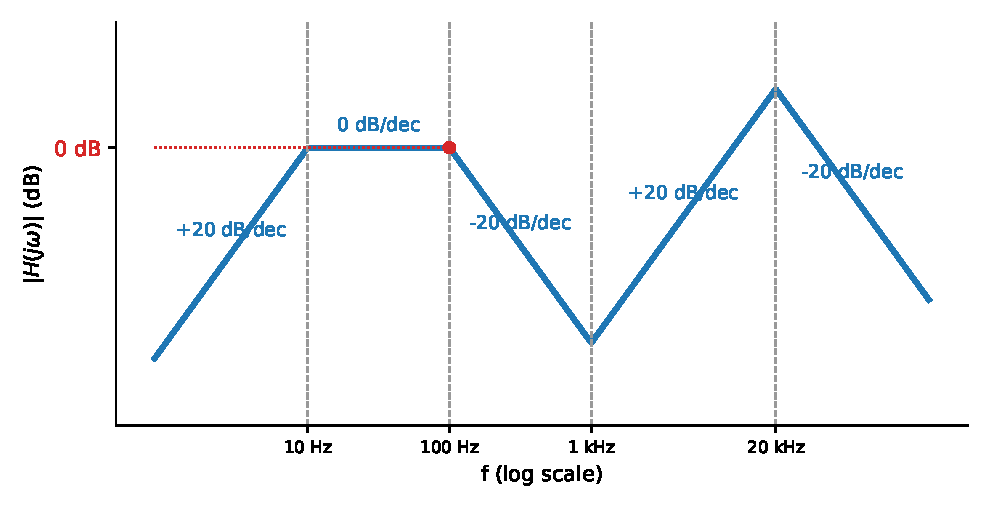
\includegraphics[width=0.7\linewidth,height=5cm,keepaspectratio]{p18_plot}\end{center}
\solstep{1}{Read the corners and slopes}Go left to right along the plot and write down the slope of every straight segment. At each corner frequency the slope changes by a multiple of 20\,dB/dec: every $-20$ is one pole, every $+20$ is one zero (tool T6 read backwards).\begin{center}\renewcommand{\arraystretch}{1.35}
\begin{tabular}{ccccl}
\toprule
corner $f_c$ & slope before & slope after & change & meaning \\
\midrule
10 Hz & $+20$ & $0$ & $-20$ & one pole at $f_c$ \\
100 Hz & $0$ & $-20$ & $-20$ & one pole at $f_c$ \\
1 kHz & $-20$ & $+20$ & $+40$ & two zeros at $f_c$ \\
20 kHz & $+20$ & $-20$ & $-40$ & two poles at $f_c$ \\
\bottomrule
\end{tabular}\end{center}

\solstep{2}{Starting slope $\Rightarrow$ factors of $s$}The plot starts with a slope of $+20$\,dB/dec, i.e. $|H|\propto\omega^1$ at low frequency: the numerator contains $s$. As in class, pair each $s$ with one of the \emph{lowest} poles (10 Hz) as $\frac{s}{s+p}$: such a factor rises at $+20$\,dB/dec below $p$ and is $\approx1$ (0\,dB) above it. The remaining poles are written $\frac{1}{1+s/p}$ and the zeros $\left(1+\frac{s}{z}\right)$. Every corner is an angular frequency $\omega_c=2\pi f_c$.
\solstep{3}{Assemble $H(s)$}Put one factor per pole/zero in front of an unknown constant $K$:\[
H(s) = K\,\dfrac{s}{s+2\pi\cdot 10}\,\dfrac{1}{1+\dfrac{s}{2\pi\cdot 100}}\,\left(1+\dfrac{s}{2\pi\cdot 1\mathrm{k}}\right)\,\left(1+\dfrac{s}{2\pi\cdot 1\mathrm{k}}\right)\,\dfrac{1}{1+\dfrac{s}{2\pi\cdot 20\mathrm{k}}}\,\dfrac{1}{1+\dfrac{s}{2\pi\cdot 20\mathrm{k}}}
\]

\solstep{4}{Find $K$ from the marked level}The plot marks the level $0$\,dB at $f=$\,100 Hz. On the straight-line plot every factor is either exactly 0\,dB (where it is $\approx1$) or a $\pm20$\,dB/dec line, so evaluate the \emph{asymptote} of each factor at that frequency (the level of a line with slope $\pm20$\,dB/dec is $\pm20\log_{10}(f/f_c)$):\begin{center}\renewcommand{\arraystretch}{1.35}
\begin{tabular}{cccc}
\toprule
factor & $f_c$ & at $f=$\,100 Hz & asymptote (dB) \\
\midrule
$\rule[-1.1em]{0pt}{2.8em}\dfrac{s}{s+2\pi\cdot 10}$ & 10 Hz & $f>f_c$: $\approx 1$ & $0$ \\
$\rule[-1.7em]{0pt}{4em}\dfrac{1}{1+\dfrac{s}{2\pi\cdot 100}}$ & 100 Hz & $f<f_c$: $\approx 1$ & $0$ \\
$\rule[-1.1em]{0pt}{2.8em}\left(1+\dfrac{s}{2\pi\cdot 1\mathrm{k}}\right)$ & 1 kHz & $f<f_c$: $\approx 1$ & $0$ \\
$\rule[-1.1em]{0pt}{2.8em}\left(1+\dfrac{s}{2\pi\cdot 1\mathrm{k}}\right)$ & 1 kHz & $f<f_c$: $\approx 1$ & $0$ \\
$\rule[-1.7em]{0pt}{4em}\dfrac{1}{1+\dfrac{s}{2\pi\cdot 20\mathrm{k}}}$ & 20 kHz & $f<f_c$: $\approx 1$ & $0$ \\
$\rule[-1.7em]{0pt}{4em}\dfrac{1}{1+\dfrac{s}{2\pi\cdot 20\mathrm{k}}}$ & 20 kHz & $f<f_c$: $\approx 1$ & $0$ \\
\textbf{sum} &  &  & $\mathbf{0}$ \\
\bottomrule
\end{tabular}\end{center}
The dB values of the factors \emph{add} (magnitudes multiply), so\[
20\log_{10}K = 0 - (0) = 0\ \mathrm{dB}\quad\Rightarrow\quad K = 10^{0/20} = 1
\]

So\[
\boxed{H(s) = 1\,\dfrac{s}{s+2\pi\cdot 10}\,\dfrac{1}{1+\dfrac{s}{2\pi\cdot 100}}\,\left(1+\dfrac{s}{2\pi\cdot 1\mathrm{k}}\right)\,\left(1+\dfrac{s}{2\pi\cdot 1\mathrm{k}}\right)\,\dfrac{1}{1+\dfrac{s}{2\pi\cdot 20\mathrm{k}}}\,\dfrac{1}{1+\dfrac{s}{2\pi\cdot 20\mathrm{k}}}}
\]

\solstep{5}{Check}Rebuild the plot from the factors: each factor's straight-line plot (green) is added to get $|H|$ (blue). It must reproduce every slope of the given plot and the marked level.\begin{center}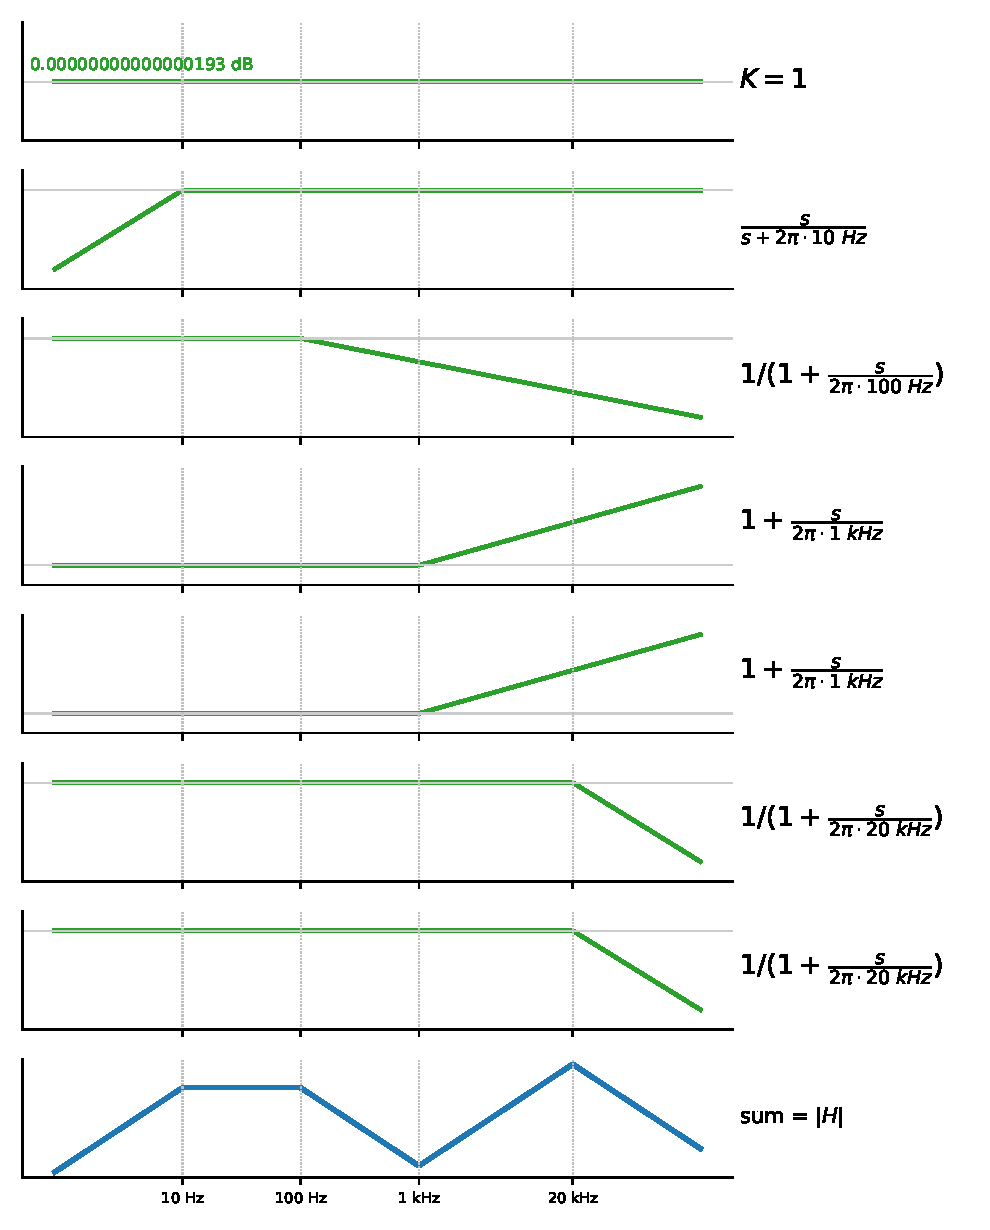
\includegraphics[width=0.82\linewidth,height=9cm,keepaspectratio]{p18_factors}\end{center}
\begin{center}\renewcommand{\arraystretch}{1.35}
\begin{tabular}{lcl}
\toprule
frequency range & slope & asymptote level \\
\midrule
$f<$ 10 Hz & $+20$ dB/dec & 0 dB at end \\
10 Hz -- 100 Hz & $0$ dB/dec & 0 dB at start, 0 dB at end \\
100 Hz -- 1 kHz & $-20$ dB/dec & 0 dB at start, -20 dB at end \\
1 kHz -- 20 kHz & $+20$ dB/dec & -20 dB at start, 6.02 dB at end \\
$f>$ 20 kHz & $-20$ dB/dec & 6.02 dB at start \\
\bottomrule
\end{tabular}\end{center}

\solstep{6}{Steady-state output}The input is $V_i(t) = 0.5\sin\left(2\pi\cdot 3000\,t\right)$, so $\omega_{in} = 2\pi\cdot 3000 = 18800$\,rad/s. Put $s=j\omega_{in}$ in each factor (tool T5; use the \emph{exact} factors here, not the straight lines): magnitudes multiply, angles add.
{\small Rules: $\left|\frac{s}{s+p}\right| = \frac{\omega}{\sqrt{\omega^2+p^2}}$, $\angle = \frac{\pi}{2}-\tan^{-1}\frac{\omega}{p}$;\quad $\left|\frac{1}{1+s/p}\right| = \frac{1}{\sqrt{1+(\omega/p)^2}}$, $\angle = -\tan^{-1}\frac{\omega}{p}$;\quad $\left|1+\frac{s}{z}\right| = \sqrt{1+(\omega/z)^2}$, $\angle = \tan^{-1}\frac{\omega}{z}$;\quad a negative $K$ adds $-\pi$.}
\begin{center}\renewcommand{\arraystretch}{1.35}
\begin{tabular}{ccc}
\toprule
factor & magnitude & angle (rad) \\
\midrule
$1$ & $1$ & $0$ \\
$\rule[-1.1em]{0pt}{2.8em}\dfrac{s}{s+2\pi\cdot 10}$ & $1$ & $0.00333$ \\
$\rule[-1.7em]{0pt}{4em}\dfrac{1}{1+\dfrac{s}{2\pi\cdot 100}}$ & $0.03331$ & $-1.54$ \\
$\rule[-1.1em]{0pt}{2.8em}\left(1+\dfrac{s}{2\pi\cdot 1\mathrm{k}}\right)$ & $3.162$ & $1.25$ \\
$\rule[-1.1em]{0pt}{2.8em}\left(1+\dfrac{s}{2\pi\cdot 1\mathrm{k}}\right)$ & $3.162$ & $1.25$ \\
$\rule[-1.7em]{0pt}{4em}\dfrac{1}{1+\dfrac{s}{2\pi\cdot 20\mathrm{k}}}$ & $0.9889$ & $-0.149$ \\
$\rule[-1.7em]{0pt}{4em}\dfrac{1}{1+\dfrac{s}{2\pi\cdot 20\mathrm{k}}}$ & $0.9889$ & $-0.149$ \\
\textbf{total} & $\mathbf{0.3258}$ (product) & $\mathbf{0.666}$ (sum) \\
\bottomrule
\end{tabular}\end{center}

\begin{align*}
|H(j\omega_{in})| &= 0.326, \qquad \angle H(j\omega_{in}) = 0.666\ \mathrm{rad} \\
v_{o,ac}(t) &= 0.326\times 0.5\,\sin\left(2\pi\cdot 3000\,t + 0.666\right) = 0.163\,\sin\left(2\pi\cdot 3000\,t + 0.666\right)
\end{align*}

\[
\boxed{V_o(t) = 0.163\,\sin\left(2\pi\cdot 3000\,t + 0.666\right)\ \mathrm{V}}
\]

\begin{ansbox}
$H(s) = 1\,\dfrac{s}{s+2\pi\cdot 10}\,\dfrac{1}{1+\dfrac{s}{2\pi\cdot 100}}\,\left(1+\dfrac{s}{2\pi\cdot 1\mathrm{k}}\right)\,\left(1+\dfrac{s}{2\pi\cdot 1\mathrm{k}}\right)\,\dfrac{1}{1+\dfrac{s}{2\pi\cdot 20\mathrm{k}}}\,\dfrac{1}{1+\dfrac{s}{2\pi\cdot 20\mathrm{k}}}$\quad (corners: 10 Hz, 100 Hz, 1 kHz, 1 kHz, 20 kHz, 20 kHz)\\[4pt]
$V_o(t) = 0.163\,\sin\left(2\pi\cdot 3000\,t + 0.666\right)\ \mathrm{V}$
\end{ansbox}

\end{document}
